\PassOptionsToPackage{unicode}{hyperref}
\PassOptionsToPackage{hyphens}{url}

\documentclass{report}
\usepackage[utf8]{inputenc}
\usepackage[italian]{babel}
\usepackage[linktoc=all]{hyperref}
\usepackage{graphicx}
\usepackage{mathtools}
\usepackage{float}
\usepackage{wrapfig}
\usepackage{tabularx}
\usepackage{xcolor}

\graphicspath{ {./images/} }
\hypersetup{
	colorlinks,
	citecolor=black,
	filecolor=black,
	linkcolor=black,
	urlcolor=black
}
\usepackage[a4paper,includeheadfoot,margin=2.54cm]{geometry}
\usepackage{fancyhdr}
\newcommand\hr{\par\vspace{-.5\ht\strutbox}\noindent\hrulefill\par}
\usepackage{enumitem}
\newcommand{\code}{\texttt}

\IfFileExists{xurl.sty}{\usepackage{xurl}}{} % add URL line breaks if available
\IfFileExists{bookmark.sty}{\usepackage{bookmark}}{\usepackage{hyperref}}
\hypersetup{
  hidelinks,
  pdfcreator={LaTeX via pandoc}}
\urlstyle{same} % disable monospaced font for URLs

\begin{document}
	
	\begin{titlepage}
	\centering
	
\includegraphics[width=0.7\textwidth]{logounitn.eps}

	\vspace{1.6cm}
	\LARGE{Dipartimento di Ingegneria e Scienza dell'Informazione\\}

	\vspace{1cm}
	\Large{Corso di Laurea in\\ Ingegneria dell'Informazione e Organizzazione d'Impresa}

	\vspace{1cm}
	\Huge\textsc{Appunti di Reti\\}
	\large{Dal materiale del prof. F. Granelli}

	\vspace{2cm}
	\Large{Autore}\\
	\large{Davide Parpinello}
	\\
	\vspace{2cm}
	\LARGE{Anno accademico 2019-2020}
	\end{titlepage}
	
	\tableofcontents
	\renewcommand{\chaptermark}[1]{%
		\markboth{#1}{}}
	\addtocontents{toc}{\protect\hypertarget{toc}{}}
	\pagestyle{fancy}
	\fancyhf{}
	\rhead{\hyperlink{toc}{Reti}}
	\lhead{\leftmark}
	\rfoot{\thepage}
	
	\chapter{Roadmap}
	\section{Internet}
	
	Internet è costituito da milioni di dispositivi, chiamati \textbf{sistemi terminali}, collegati tra loro da collegamenti in rame, fibre ottiche, oppure via radio come onde elettromagnetiche o satelliti.
	\medskip\\
	La frequenza di trasmissione in internet è data dall'ampiezza di banda disponibile.
	\medskip\\Sulla rete internet inoltre sono presenti particolari host, denominati \textbf{router}, che si occupano di instradare i pacchetti verso la loro destinazione finale.
	\medskip\\Nello scambio di messaggi tra host vengono implementati dei \textbf{protocolli}, che ne definiscono formato e ordine d'invio, così come le azioni intraprese in fase di trasmissione e/o ricezione di un messaggio o un altro evento.
	\medskip\\Internet è un'infrastruttura di comunicazione per applicazione distribuita, viene anche chiamato "rete delle reti" ed è organizzato in modo gerarchico.
	\section{Ai confini della rete}
	Sul bordo della rete internet troviamo applicazioni e sistemi terminali, raggruppati tra loro e connessi tra di loro mediante collegamenti cablati e wireless.
	\medskip\\I sistemi terminali (o host) fanno girare diversi programmi applicativi e possono essere organizzati con architettura client/server oppure P2P.
	\medskip\\L'accesso a internet può avvenire mediante diversi modi:
	\begin{itemize}
		\item \textbf{Accesso residenziale:} viene utilizzato un modem dial-up o DSL.
		\item \textbf{Accesso aziendale:} una LAN collega i sistemi terminali di aziende e università all'\textbf{edge router}, i sistemi terminali sono collegati tra loro mediante uno switch ethernet.
		\item \textbf{Accesso wireless:} i terminali vengono collegati mediante \textbf{access point}.
		\item \textbf{Reti domestiche:} sono costituite da un modem DSL o via cavo, un router/firewall/NAT, switch ethernet e accesso wireless. Spesso queste funzioni vengono raggruppate in un unico dispositivo (modem/router).
	\end{itemize}
	\section{Il nucleo della rete}
	Al centro della rete si trovano invece router interconnessi tra loro, che creano quindi una rete delle reti.
	\medskip\\I dati nel nucleo della rete vengono trasferiti con due modalità differenti:
	\begin{itemize}
		\item \textbf{Commutazione di circuito:} è presente un circuito dedicato per l'intera durata della sessione
		\item \textbf{Commutazione di pacchetto:} i messaggi di una sessione utilizzano le risorse su richiesta, di conseguenza potrebbero dover attendere per accedere a un collegamento.
	\end{itemize}
	\subsection{Esempio di commutazione di circuito}
	Consideriamo un file L di 640.000 bit, un bitrate totale C da 1.536 Mbps, TDM con 24 slot/s, 500ms per stabilire la connessione.
	\medskip\\ Trovo inizialmente la capacità di un singolo slot:\[C_{1 slot} = \frac{C}{24} = 0.064 Mbps = 64 Kbps\]
	Successivamente calcolo il tempo necessario alla trasmissione:\[T_{tx} = \frac{L}{C_{1 slot}} = 10s\]
	Infine, calcolo il tempo totale:\[T_{tot}=500ms+10s=10,5s\]
	\subsection{Esempio di commutazione di circuito}
	I secondi necessari per trasmettere un pacchetto in uscita su un collegamento da R bps sono dati da L/R, mentre il ritardo 3L/R
	\subsection{Confronto fra commutazione di pacchetto e di circuito}
	La commutazione di pacchetto consente un utilizzo della rete da parte di maggiori utenti, ed è ottima per i dati a raffica.\medskip\\ Dal lato negativo, presenta un'eccessiva congestione, causando ritardi e perdite di pacchetti. Sono quindi necessari protocolli per il trasferimento affidabile e per il controllo della congestione.
	\subsection{Struttura gerarchica}
	La rete internet ha una struttura fondamentalmente gerarchica:
	\begin{itemize}
		\item Al centro sono presenti \textbf{ISP di livello 1}, che offrono una copertura nazionale e/o internazionale
		\begin{itemize}
			\item Comunicano tra loro come fossero pari
		\end{itemize}
		\item \textbf{ISP di livello 2:} ISP più piccoli, copertura nazionale/distrettuale.
		\begin{itemize}
			\item Si può connettere solo ad alcuni ISP di livello 1 e ad altri di livello 2
			\item Paga l'ISP di livello 1 che gli fornisce la connettività per il resto della rete
		\end{itemize}
		\item \textbf{ISP di livello 3 e ISP locali (di accesso):}
		\begin{itemize} 
			\item sono le reti "ultimo salto", le più vicine agli host
			\item Sono clienti degli ISP di livello superiore che li collegano all'intera internet.
		\end{itemize}
	\end{itemize}
	Un pacchetto attraversa un sacco di reti, dal livello più basso fino al principale e poi nuovamente a scendere.
	\section{Ritardi, perdite e throughput nelle reti a comunicazione di pacchetto}
	Nella rete si verificano dei ritardi quando il tasso di arrivo dei pacchetti eccede la capacità di evaderli, con la conseguenza che vengono accodati nei buffer del router in attesa del proprio turno. Se non ci sono buffer liberi i pacchetti vengono scartati e ritrasmetti dal nodo precedente o, in alcuni casi, non venire proprio ritrasmessi.
	\medskip\\ Quattro cause di ritardo dei pacchetti sono le seguenti:
	\begin{enumerate}
		\item Ritardo di elaborazione sul nodo
		\begin{itemize}
			\item Controllo errori sui bit
			\item Determinazione del canale di uscita
		\end{itemize}
		\item Ritardo di accodamento
		\begin{itemize}
			\item Attesa di trasmissione
			\item Livello di congestione del router
		\end{itemize}
		\item Ritardo di trasmissione (L/R)
		\begin{itemize}
			\item R = frequenza di trasmissione del collegamento
			\item L = lunghezza del pacchetto
		\end{itemize}
		\item Ritardo di propagazione (d/s)
		\begin{itemize}
			\item d = lunghezza dl collegamento fisico 
			\item s = velocità di propagazione del collegamento (\textasciitilde \(2 \cdot 10^8\) m/s)
		\end{itemize}
	\end{enumerate}
	\begin{center}
		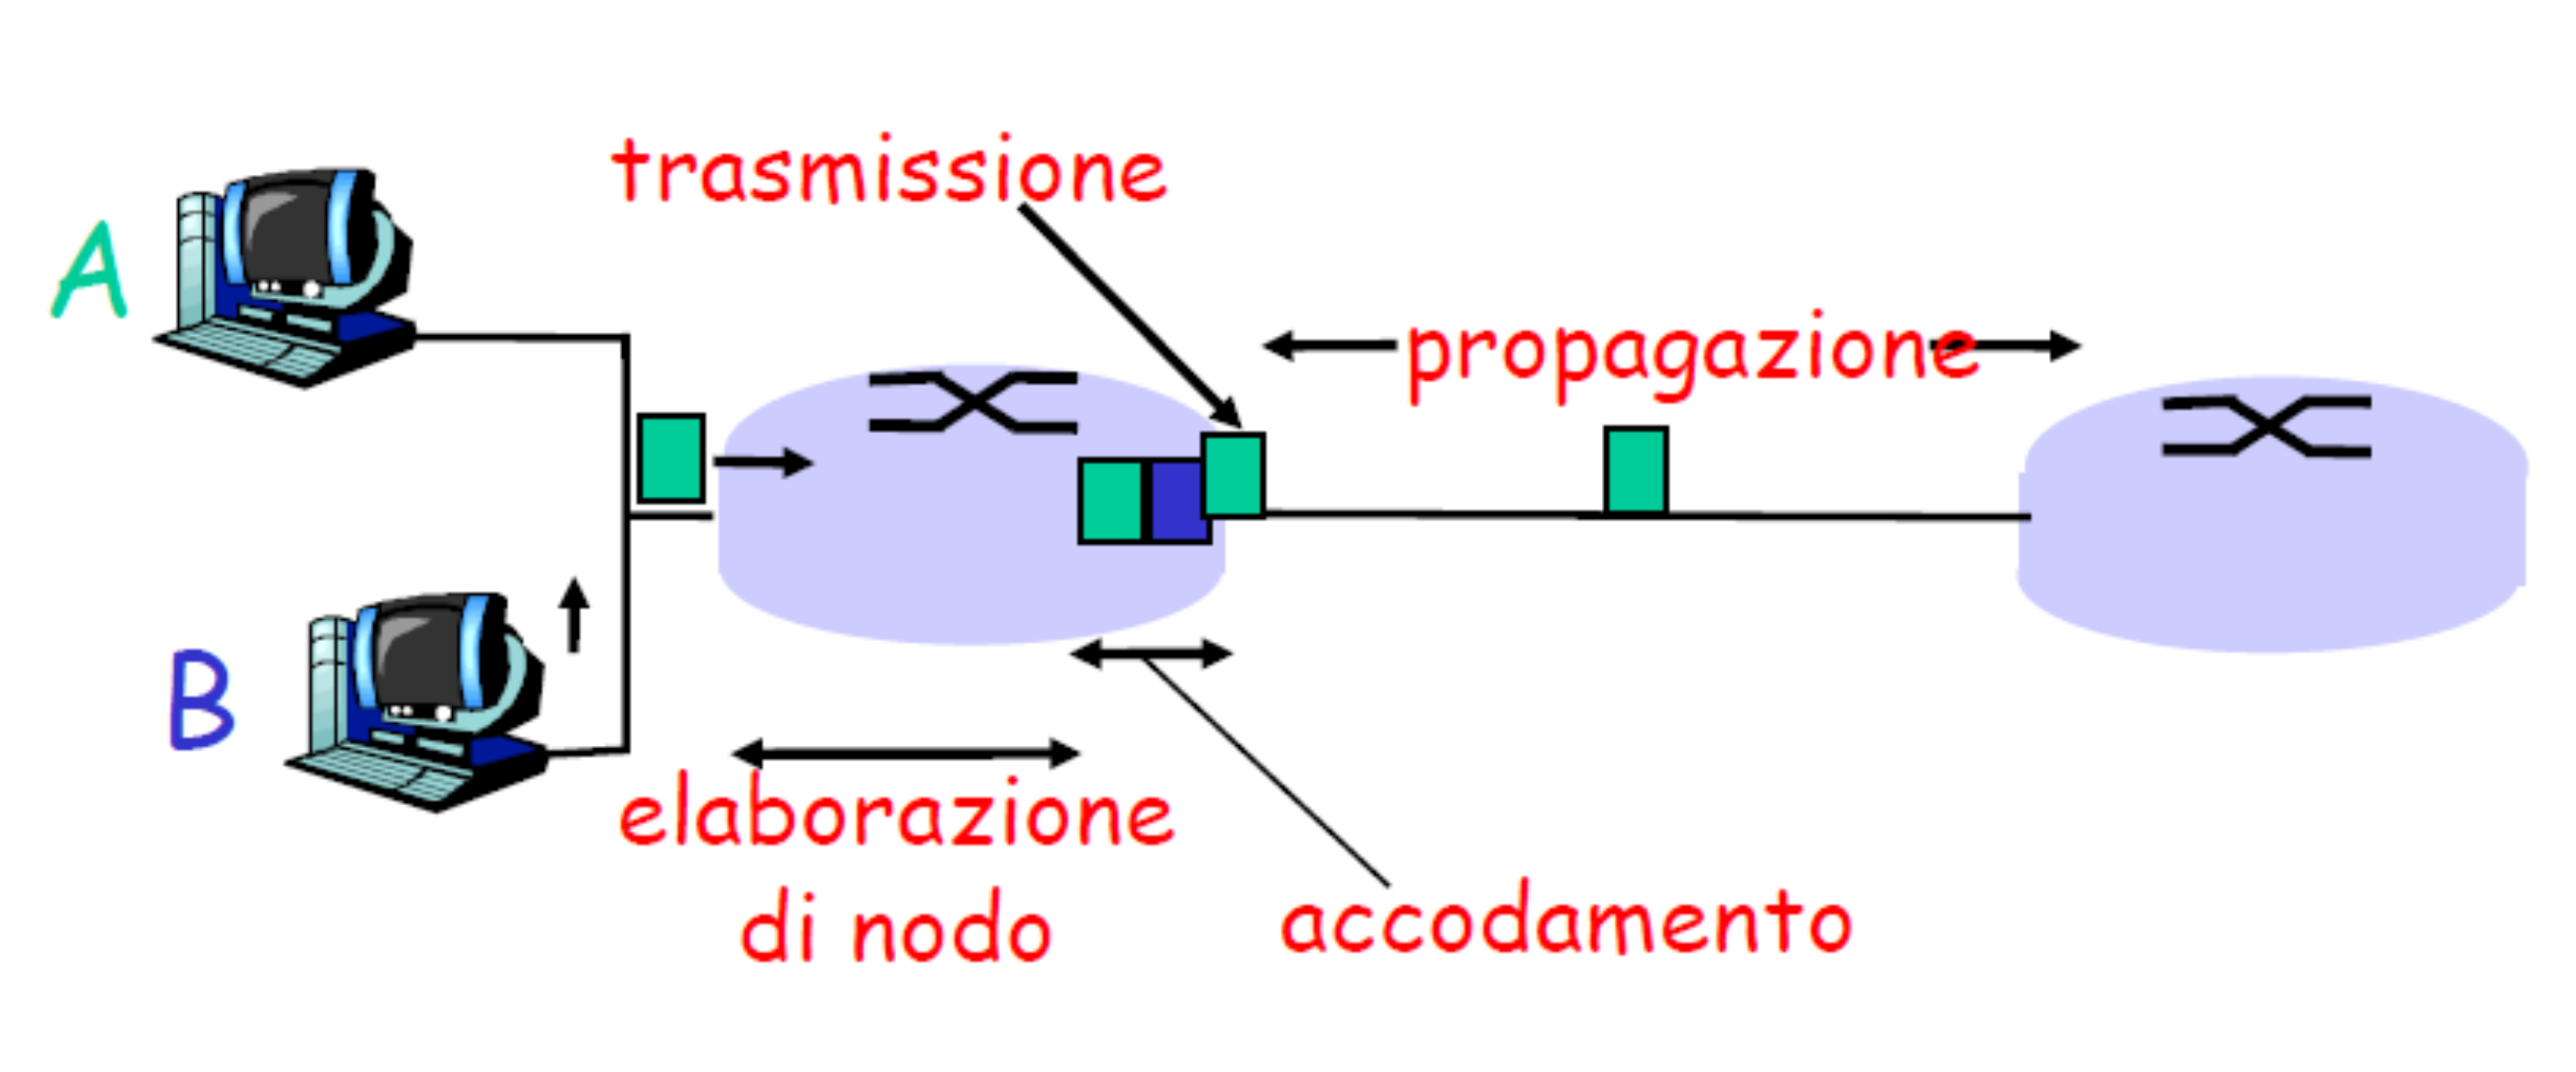
\includegraphics[width=0.7\linewidth]{ritardi.png}
	\end{center}
	\subsection{Ritardo di un nodo}
	Il ritardo di un nodo è dato dalla seguente formula:
	\begin{equation}
		d_{nodal} = d_{proc}+d_{queue}+d_{trans}+d_{prop}
	\end{equation}
	dove:
	\begin{itemize}
		\item d\textsubscript{proc} = ritardo di elaborazione (processing delay)
		\subitem- in genere di pochi microsecondi, o anche meno
		\item d\textsubscript{queue} = ritardo di accodamento
		\subitem- dipende dalla congestione
		\item d\textsubscript{trans} = ritardo di trasmissione (transmission delay)
		\subitem- significativo sui collegamenti a bassa velocità
		\item d\textsubscript{prop} = ritardo di propagazione (propagation delay)
		\subitem- da pochi microsecondi a centinaia di millisecondi
	\end{itemize}
	\subsubsection{Ritardo di accodamento}
	\begin{itemize}
		\item R = frequenza di trasmissione (bps)
		\item L = lunghezza del pacchetto (bit)
		\item a = tasso medio di arrivo dei pacchetti
	\end{itemize}
	
	Se calcoliamo La/R otteniamo l'intensità di traffico:
	\begin{itemize}
		\item Vicino a 0: poco ritardo
		\item Minore o uguale a 1: traffico consistente
		\item Maggiore di 1: più lavoro in arrivo di quanto possa essere effettivamente svolto, ritardo medio infinito.
	\end{itemize}
	Il \textbf{throughput} viene calcolato come la frequenza (bit/unità di tempo) alla quale i bit sono trasferiti tra mittente e ricevente. Può essere istantaneo o medio (in un periodo più lungo).
	\medskip\\In internet si considera anche il \textbf{collo di bottiglia}, ovvero un collegamento su un percorso punto-punto che vincola un throughput end to end.
	\section{Livelli di protocollo e i loro modelli di servizio}
	Si considerano principalmente 5 livelli di protocollo:
	\begin{enumerate}
		\item \textbf{Applicazione:} di supporto alle applicazioni di rete
		\item \textbf{Trasporto:} trasferimento dei messaggi del livello applicazione tra modulo client e server, connessione tra processi applicativi
		\item \textbf{Rete:} instradamento dei datagram dall'origine al destinatario
		\item \textbf{Link \textit{(collegamento)}:} instradamento dei datagram attraverso una serie di commutatori di pacchetto
		\item \textbf{Fisico:} trasferimento dei singoli bit
	\end{enumerate}
	\section{Reti sotto attacco: la sicurezza}
	I malintenzionati installano malware negli host attraverso internet. Il malware può raggiungere gli host attraverso virus, worm o cavalli di Troia. Un malware di spionaggio può registrare quanto viene digitato, i siti visitati e informazioni di upload. Gli host infettati possono diventare botnet e essere usati per lo spamming e attacchi DDoS. Un malware è spesso auto-replicante e da un host attaccato può passare ad altri host.
	\paragraph{Analisi di pacchetti} Chiamato anche packet sniffing, quando un'interfaccia di rete legge/registra tutti i pacchetti che la attraversano.
	\paragraph{IP spoofing} Invio di pacchetti con un indirizzo sorgente falso.
	\paragraph{Record-and-playback} Vengono "sniffati" dati sensibili per utilizzarli in un secondo momento.
	\chapter{Il livello Applicazione}
	\section{Principi delle applicazioni di rete}
	Le applicazioni di rete sono costruite con diverse architetture
	\begin{itemize}
		\item Client-Server
		\begin{itemize}
			\item L'host (o client) interagisce direttamente con il server
			\item Più client ci sono più il servizio diminuisce
		\end{itemize}
		\item Peer-to-Peer (P2P)
		\begin{itemize}
			\item Non c'è un server sempre attivo
			\item Coppie arbitrarie di host comunicano direttamente fra di loro
			\item Facilmente scalabile ma difficile da gestire
		\end{itemize}
		\item Architetture ibride
		\begin{itemize}
			\item Skype, messaggistica istantanea
			\item Connessione client-client, utilizzo del server per la ricerca dell'indirizzo della parte remota
		\end{itemize}
		\item Cloud computing
		\begin{itemize}
			\item Un insieme di tecnologie che permettono sia di archiviare dati che elaborarli tramite l'utilizzo di risorse distribuite e virtualizzate in rete
			\item Creazione di copie di sicurezza preventive in modo automatico trasferendo tutta l'operatività online
			\item Dati memorizzati in server farm
			\item Sempre client-server ma basata sulla virtualizzazione
		\end{itemize}
	\end{itemize}
	Un processo è un programma in esecuzione su un host. All'interno dell'host due processi comunicano utilizzando schemi di interprocesso, mentre su host differenti comunicano attraverso lo scambio di messaggi.
	\begin{itemize}
		\item \textbf{Processo client:} processo che dà inizio alla comunicazione
		\item \textbf{Processo server:} processo che attende di essere contattato
	\end{itemize}
	Un processo invia/riceve messaggi mediante la sua socket. La socket è analoga ad una porta mediante la quale un processo che vuole inviare un messaggio lo fa uscire. Questo presuppone l’esistenza di un’infrastruttura esterna che trasporterà il messaggio attraverso la rete fino alla porta del processo di destinazione.
	\medskip\\ Per il trasporto internet vengono utilizzati i servizi dei protocolli TCP e UDP.
	\subsubsection{Servizio TCP}
	\begin{itemize}
		\item \textcolor{red}{Orientato alla connessione:} è richiesto un setup fra i processi client e server
		\item \textcolor{red}{Trasporto affidabile} fra i processi d'invio e ricezione
		\item \textcolor{red}{Controllo di flusso:} il mittente non vuole sovraccaricare il destinatario
		\item \textcolor{red}{Controllo della congestione:} "strozza" il processo d'invio quando la rete è sovraccaricata
		\item \textbf{Non offre} temporizzazione, garanzie sull'ampiezza di banda minima, sicurezza
		\item \textbf{Più affidabile ma si paga con ritardi di trasferimento}
	\end{itemize}
	\subsubsection{Servizio UDP}
	\begin{itemize}
		\item Trasferimento dati inaffidabile fra processi d'invio e ricezione
		\item \textbf{Non offre} setup della connessione, affidabilità, controllo di flusso, controllo della congestione, temporizzazione né ampiezza di banda minima e sicurezza
		\item \textcolor{red}{Mandare i dati il più velocemente possibile ma senza completa affidabilità}, usato per gaming online e VoIP
	\end{itemize}
	\section{Web e HTTP}
	L'HTTP, o HyperText Transfer Protocol, è un protocollo a livello applicazione per il web, che considera un client che richiede, riceve e visualizza gli oggetti del Web e un server, che invia gli oggetti in risposta ad una richiesta.
	\medskip\\Viene utilizzato TCP nel seguente modo:
	\begin{itemize}
		\item Il client inizializza la connessione TCP con il server (crea una socket) tipicamente sulla porta 80
		\item Il server accetta la connessione TCP dal client
		\item Avviene lo scambio di messaggi HTTP tra browser e server web
		\item Chiusura della connessione TCP
	\end{itemize}
	HTTP è un protocollo \textit{stateless} (senza stato), cioè il server non mantiene informazioni sulle richieste fatte dal client.
	\medskip\\Le connessioni HTTP possono essere non persistenti o persistenti.
	\paragraph{RTT} Round trip time, tempo impiegato da un piccolo pacchetto per andare dal client al server e ritornare al client.
	\subsection{Connessioni non persistenti}
	Viene trasferito un solo oggetto su una singola connessione TCP. Il tempo di risposta è dato da:
	\begin{itemize}
		\item Un RTT per inizializzare la connessione TCP
		\item Un RTT per inviare la richiesta HTTP e i primi byte
		\item Il tempo necessario alla trasmissione del file
	\end{itemize}
	Quindi totale = 2 RTT + tempo di trasmissione. Le connessioni non persistenti presentano alcuni svantaggi:
	\begin{itemize}
		\item Richiedono 2RTT per ogni oggetto
		\item Overhead dell'OS per ogni connessione TCP
		\item I browser aprono spesso connessioni TCP parallele per caricare gli oggetti referenziati
	\end{itemize}
	\subsection{Connessioni persistenti}
	Il server lascia la connessione TCP aperta dopo l'invio di una risposta, i successivi messaggi tra gli stessi client/server vengono trasmessi sulla connessione aperta, il client invia le richieste non appena incontra un oggetto referenziato, un solo RTT per tutti gli oggetti referenziati.
	\subsection{Messaggi HTTP}
	I messaggi HTTP possono essere di richiesta o di risposta.
	\subsubsection{Richiesta HTTP}
	\begin{verbatim}
		GET /somedir/page.html HTTP/1.1
		Host: www.someschool.edu
		User-agent: Mozilla/4.0
		Connection: close Accept-language:fr
	\end{verbatim}
	\subsubsection{Tipi di metodi}
	La versione HTTP/1.0 fornisce i seguenti metodi per effettuare le richiese:
	\begin{itemize}
		\item \textbf{GET:} richiesta solamente mediante URL
		\item \textbf{POST:} vengono inseriti nel corpo della richiesta anche dati da inviare al server
		\item \textbf{HEAD:} chiede al server di escludere l'oggetto richiesto dalla risposta
	\end{itemize}
	Nella versione HTTP/1.1 vengono aggiunti i seguenti metodi:
	\begin{itemize}
		\item \textbf{PUT:} include il file nel corpo dell'entità e lo invia al percorso specificato nel campo URL
		\item \textbf{DELETE:} cancella il file specificato nel campo URL
	\end{itemize}
	\subsubsection{Risposta HTTP}
	\begin{verbatim}
		HTTP/1.1 200 OK
		Connection close
		Date: Thu, 06 Aug 1998 12:00:15 GMT
		Server: Apache/1.3.0 (Unix)
		Last-Modified: Mon, 22 Jun 1998 ...
		Content-Length: 6821
		Content-Type: text/html
	\end{verbatim}
	\subsubsection{Codici di stato della risposta HTTP}
	Nella prima riga del messaggio di risposta sono inclusi codice di stato e relativa espressione in base all'esito della richiesta. Alcuni codici sono i seguenti:
	\begin{itemize}
		\item \textbf{200 OK:} La richiesta ha avuto successo, oggetto inviato nella risposta
		\item \textbf{301 Moved Permanently:} Oggetto trasferito nella nuova posizione indicata da \verb|Location|
		\item \textbf{400 Bad Request:} il messaggio di richiesta non è stato compreso dal server
		\item \textbf{404 Not Found:} il documento richiesto non si trova su questo server
		\item \textbf{505 HTTP Version Not Supported:} il server non ha la versione di protocollo HTTP indicata
	\end{itemize}
	\subsection{Cookies}
	\begin{center}
		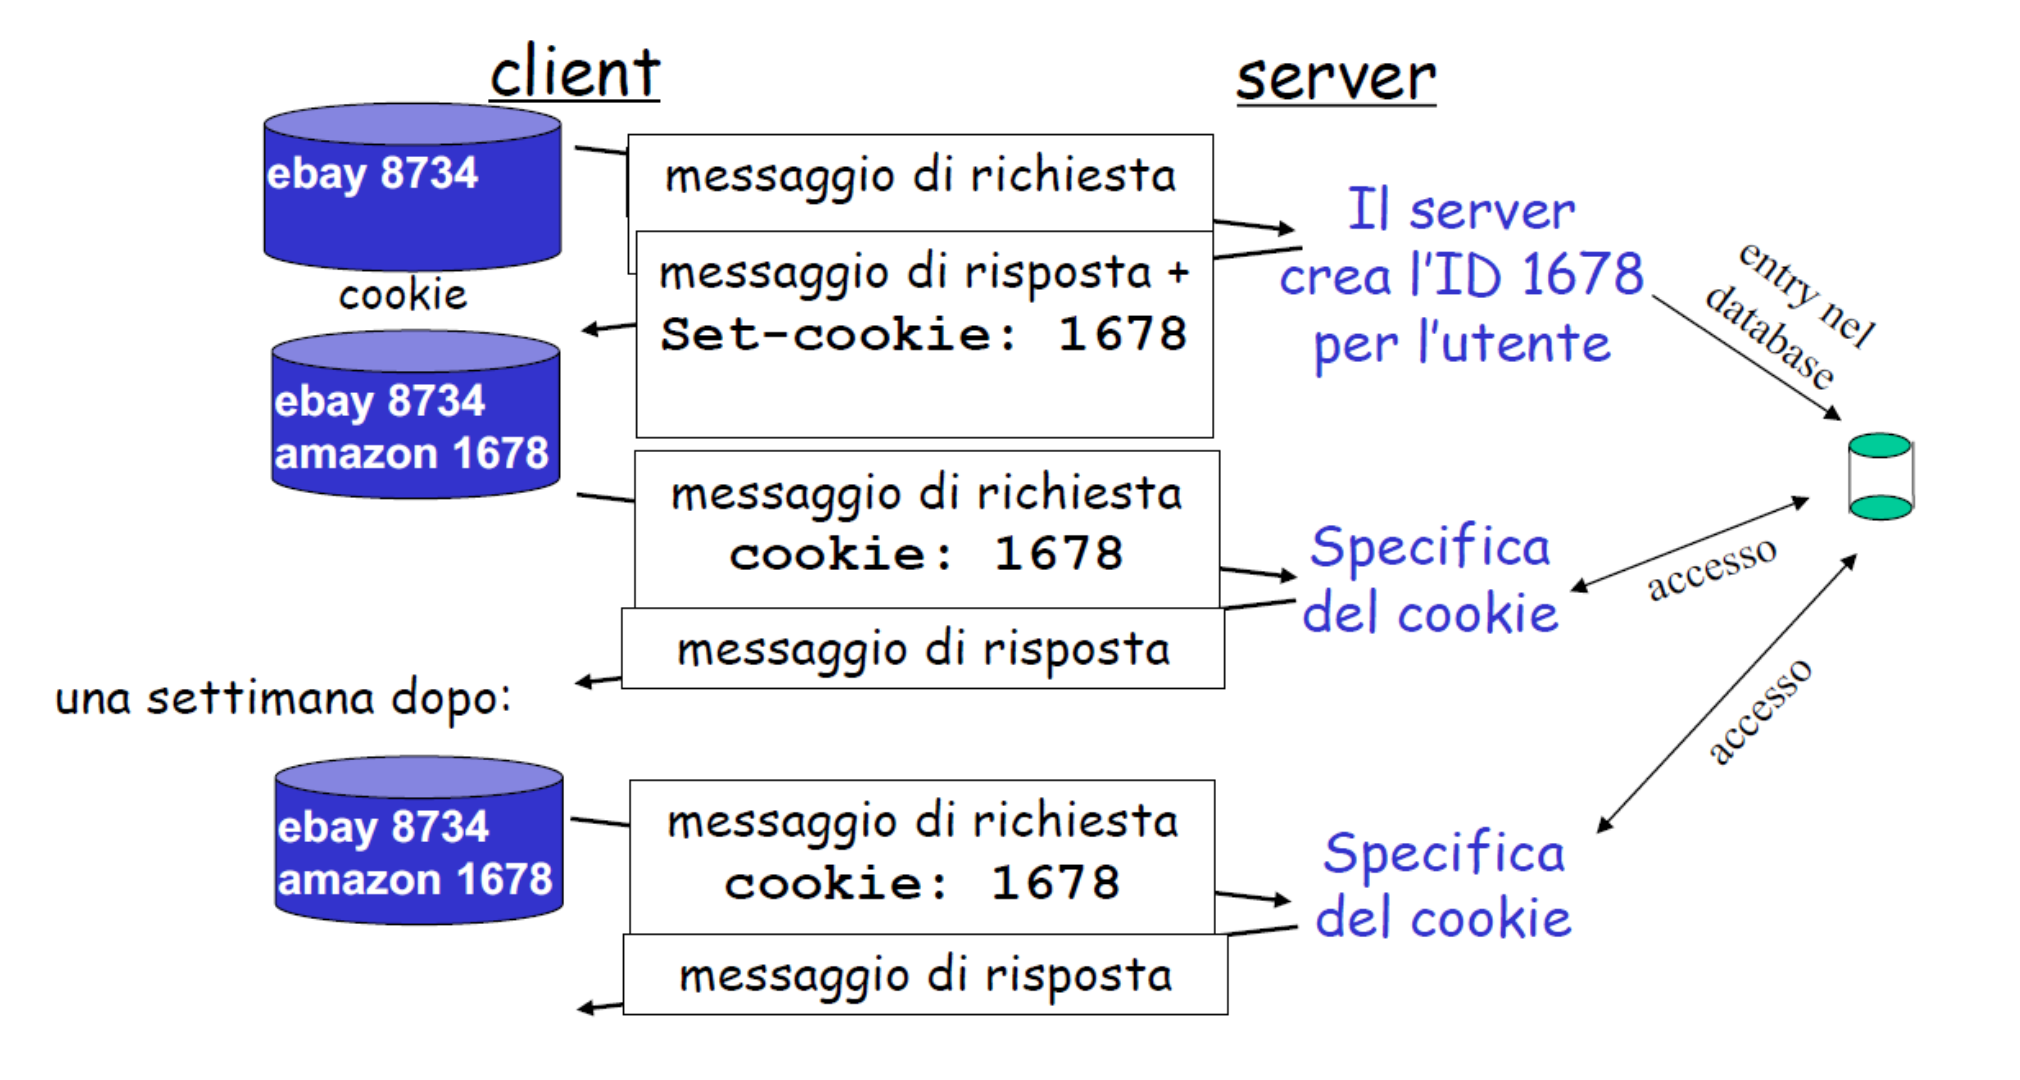
\includegraphics[width=0.7\linewidth]{cookies.png}
	\end{center}
	I cookies possono essere utilizzati per: autorizzazioni, dati carte per acquisti, raccomandazioni all'utente e possono mantenere lo stato del mittente e del ricevente per più transazioni; i messaggi HTTP trasportano lo stato. I cookies permettono ai siti di imparare molte cose sugli utenti.
	\subsection{Cache web (server proxy)}
	L'obiettivo di una web cache è quello di soddisfare la richiesta del client senza coinvolgere il server d'origine. La cache opera come client e come server, e consente di ridurre i tempi di risposta alle richieste dei client, riducendo il traffico sul collegamento a internet.
	\paragraph{GET condizionale} Ha l'obiettivo di non inviare un oggetto se la cache ne ha una copia aggiornata. 
	\\Per questo la cache specifica la data della copia dell'oggetto nella richiesta HTTP: \verb|If-modified-since: <date>|
	\\A lato server la risposta non contiene l'oggetto se la copia nella cache è aggiornata: \verb|HTTP/1.0 304 not modified|
	\subsection{HTTP/2.0}
	È un’evoluzione di HTTP, che mantiene quindi i metodi HTTP, i codici di stato e la semantica migliorando però le prestazioni.
	\section{FTP}
	FTP, o File Transfer Protocol, viene utilizzato per trasferire file con un host remoto. Il server FTP opera solitamente sulla porta 21. Vengono aperte due connessioni, prima una di controllo e successivamente, se andata a buon fine la prima, una seconda per il trasferimento del file. La connessione di controllo è quindi "fuori banda" (out of band). Il server FTP mantiene lo stato
	\subsection{Comandi comuni}
	\begin{itemize}
		\item \verb|USER username|
		\item \verb|PASS password|
		\item \verb|LIST| elenca i file della directory corrente
		\item \verb|RETR filename| recupera un file dalla directory corrente
		\item \verb|STOR filename| memorizza un file nell'host remoto
	\end{itemize}
	\subsection{Codici di ritorno comuni}
	\begin{itemize}
		\item \verb|331 Username OK, password required|
		\item \verb|125 data connection already open; transfer starting|
		\item \verb|425 Can't open data connection|
		\item \verb|452 Error writing file|
	\end{itemize}
	\section{Posta elettronica}
	La posta elettronica è costituita da tre componenti principali: agente utente, server di posta, SMTP (Simple Mail Transfer Protocol).
	\paragraph{Agente utente} Detto anche mail reader, si occupa della composizione, editing e lettura dei messaggi di posta elettronica (esempi: Outlook, Thunderbird). I messaggi in uscita sono memorizzati sul server.
	\paragraph{Server di posta} In esso è contenuta la casella di posta (mailbox) che contiene i messaggi in arrivo per l'utente e la coda dei messaggi da trasmettere.
	\paragraph{Protocollo SMTP} Utilizzato tra i server per inviare messaggi: il client è il server di posta trasmittente e il server il ricevente. Viene utilizzato TCP per trasferire in modo affidabile i messaggi di posta dal client al server sulla porta 25; il trasferimento è diretto. Ci sono tre fasi per il trasferimento: handshaking (saluto), trasferimento dei messaggi e chiusura. L'SMTP utilizza connessioni persistenti.
	\medskip\\Esistono poi diversi protocolli di accesso alla posta:
	\begin{itemize}
		\item POP: Post Office Protocol. Utilizzato per autorizzazione e download
		\item IMAP: Internet Mail Access Protocol. Ha più funzioni e consente di manipolare i messaggi memorizzati sul server.
		\item HTTP: GMail, Hotmail, ecc...
	\end{itemize}
	\paragraph{POP3} Suddiviso in due fasi: autorizzazione e transazione, è un protocollo senza stato tra le varie sessioni
	\paragraph{IMAP} Mantiene tutti i messaggi sul server, consente all'utente di organizzare i messaggi in cartelle e conserva lo stato tra le varie sessioni (nomi delle cartelle, associazione tra identificatori dei messaggi e nomi delle cartelle).
	\section{DNS}
	Il DNS, Domain Name System è un protocollo a livello applicazione che consente a host, router e server DNS di comunicare per risolvere i nomi dei siti web. Il DNS traduce un hostname come \textit{www.facebook.com} in un indirizzo IP.
	\paragraph{Host aliasing} In alcuni casi, un host può avere più nomi, come nel caso dell'aliasing dei server mail.
	\medskip\\Il DNS è un database distribuito implementato in una gerarchia di server DNS. Tipicamente, un server DNS radice viene contattato da un server DNS locale che non può tradurre un nome. A sua volta, il DNS radice contatta un server DNS autorizzato se non conosce la mappatura del nome, la ottiene e la restituisce al server DNS locale.
	\paragraph{Server TLD (top-level domain} Si occupano dei domini .com, .org, .net, .edu, ecc. e di tutti gli altri domini locali di alto livello, quali .uk, .fr, .ca e .jp.
	\paragraph{Server di competenza (authoritative server} Ogni organizzazione dotata di host internet pubblicamente accessibili (server web e di posta) deve fornire i record DNS di pubblico dominio che mappano i nomi di tali host in indirizzi IP; possono essere mantenuti dall'organizzazione o dal service provider.
	\medskip\\Il server DNS locale non appartiene strettamente alla gerarchia dei server, ciascun ISP (università, società) ha un server DNS locale. Quando un host effettua una richiesta DNS, la query viene inviata al suo server DNS locale, che opera da proxy e inoltra la query in una gerarchia di server DNS.
	\medskip\\Le query DNS possono essere effettuate in due modalità: iterativa o ricorsiva. Nel caso di query iterativa, il server contattato risponde con il nome del server da contattare, nel caso in cui non riesca a risolvere il nome; sarà quindi compito dell'host iniziale contattare quel server. Nel caso di query ricorsiva l'host affida il compito di tradurre il nome al server DNS contattato; in questo caso sarà il server stesso a contattare un secondo server per risolvere il nome, al quale può a sua volta assegnare il compito in modo iterativo.
	\medskip\\Una volta che un server DNS impara la mappatura la mette nella cache, dove le informazioni vengono invalidate dopo un certo periodo di tempo. Tipicamente, un server DNS locale memorizza nella cache gli indirizzi IP dei server TLD, quindi i server radice non vengono visitati spesso.
	\medskip\\Il DNS è un database distribuito che memorizza i record di risorsa (RR) che hanno il seguente formato: \verb|(name, value, type, TTL)|
	\begin{itemize}
		\item Type = A
		\begin{itemize}
			\item \code{name} è il nome dell'host (server)
			\item \code{value} è l'indirizzo IP
		\end{itemize}
		\item Type = NS
		\begin{itemize}
			\item \code{name} è il dominio (\code{foo.com})
			\item \code{value} è il nome dell'host del server DNS di competenza di questo dominio
		\end{itemize}
		\item Type = CNAME
		\begin{itemize}
			\item \code{name} è il nome alias di qualche nome canonico (\code{www.ibm.com})
			\item \code{value} è il nome canonico (\code{servereast.backup2.ibm.com})
		\end{itemize}
		\item Type = MX
		\begin{itemize}
			\item \code{value} è il nome del server di posta associato a \code{name}
		\end{itemize}
	\end{itemize}
	\subsection{Protocollo DNS}
	Il protocollo DNS è costituito da domande (query) e messaggi di risposta, entrambi con lo stesso formato.
	\subsubsection{Intestazione del messaggio (12 byte - 6 campi)}
	L'intestazione è costituita da un numero da 16 bit di identificazione della domanda, utilizzato uguale dalla risposta, e da un flag indicante:
	\begin{itemize}
		\item domanda o risposta
		\item richiesta di ricorsione
		\item ricorsione disponibile
		\item risposta di competenza
	\end{itemize}
	\subsubsection{Resto del messaggio}
	\begin{itemize}
		\item Campi per il nome richiesto e il tipo di domanda
		\item RR nella risposta alla domanda
		\item Record per i server di competenza
		\item Informazioni extra che possono essere usate
	\end{itemize}
	\newpage
	\section{Condivisione di file P2P}
	Nell'architettura P2P pura non c'è un server sempre attivo, infatti coppie arbitrarie di host (peer) comunicano direttamente tra loro. I peer non devono essere sempre attivi e possono cambiare indirizzo IP.
	\subsection{Confronto tra architettura server client e P2P}
	\begin{center}
		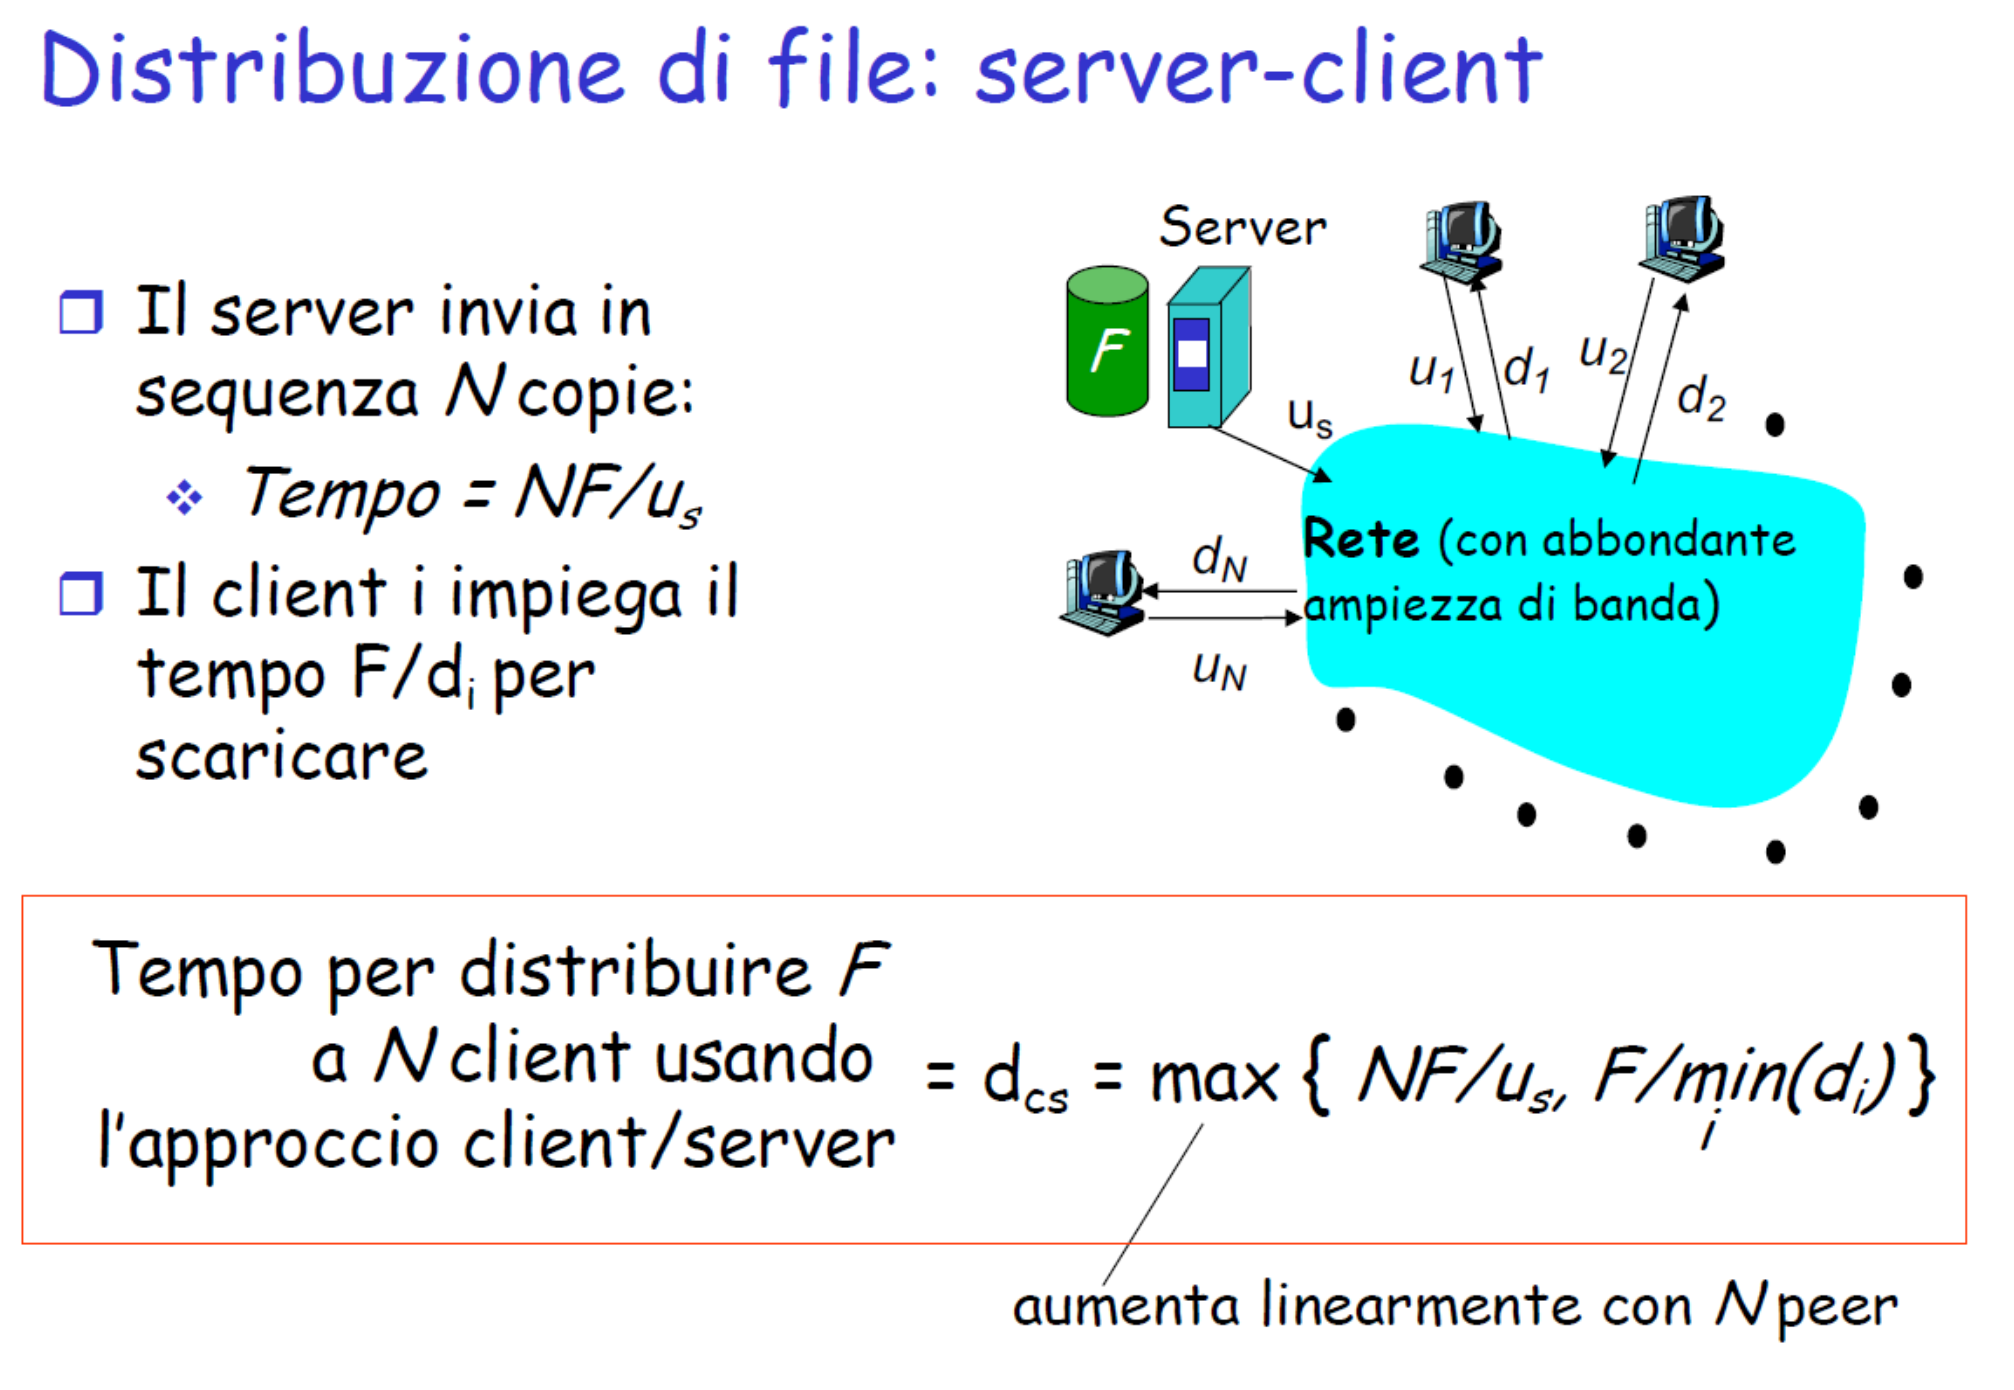
\includegraphics[width=0.7\linewidth]{server-client.png}
		\medskip\\
		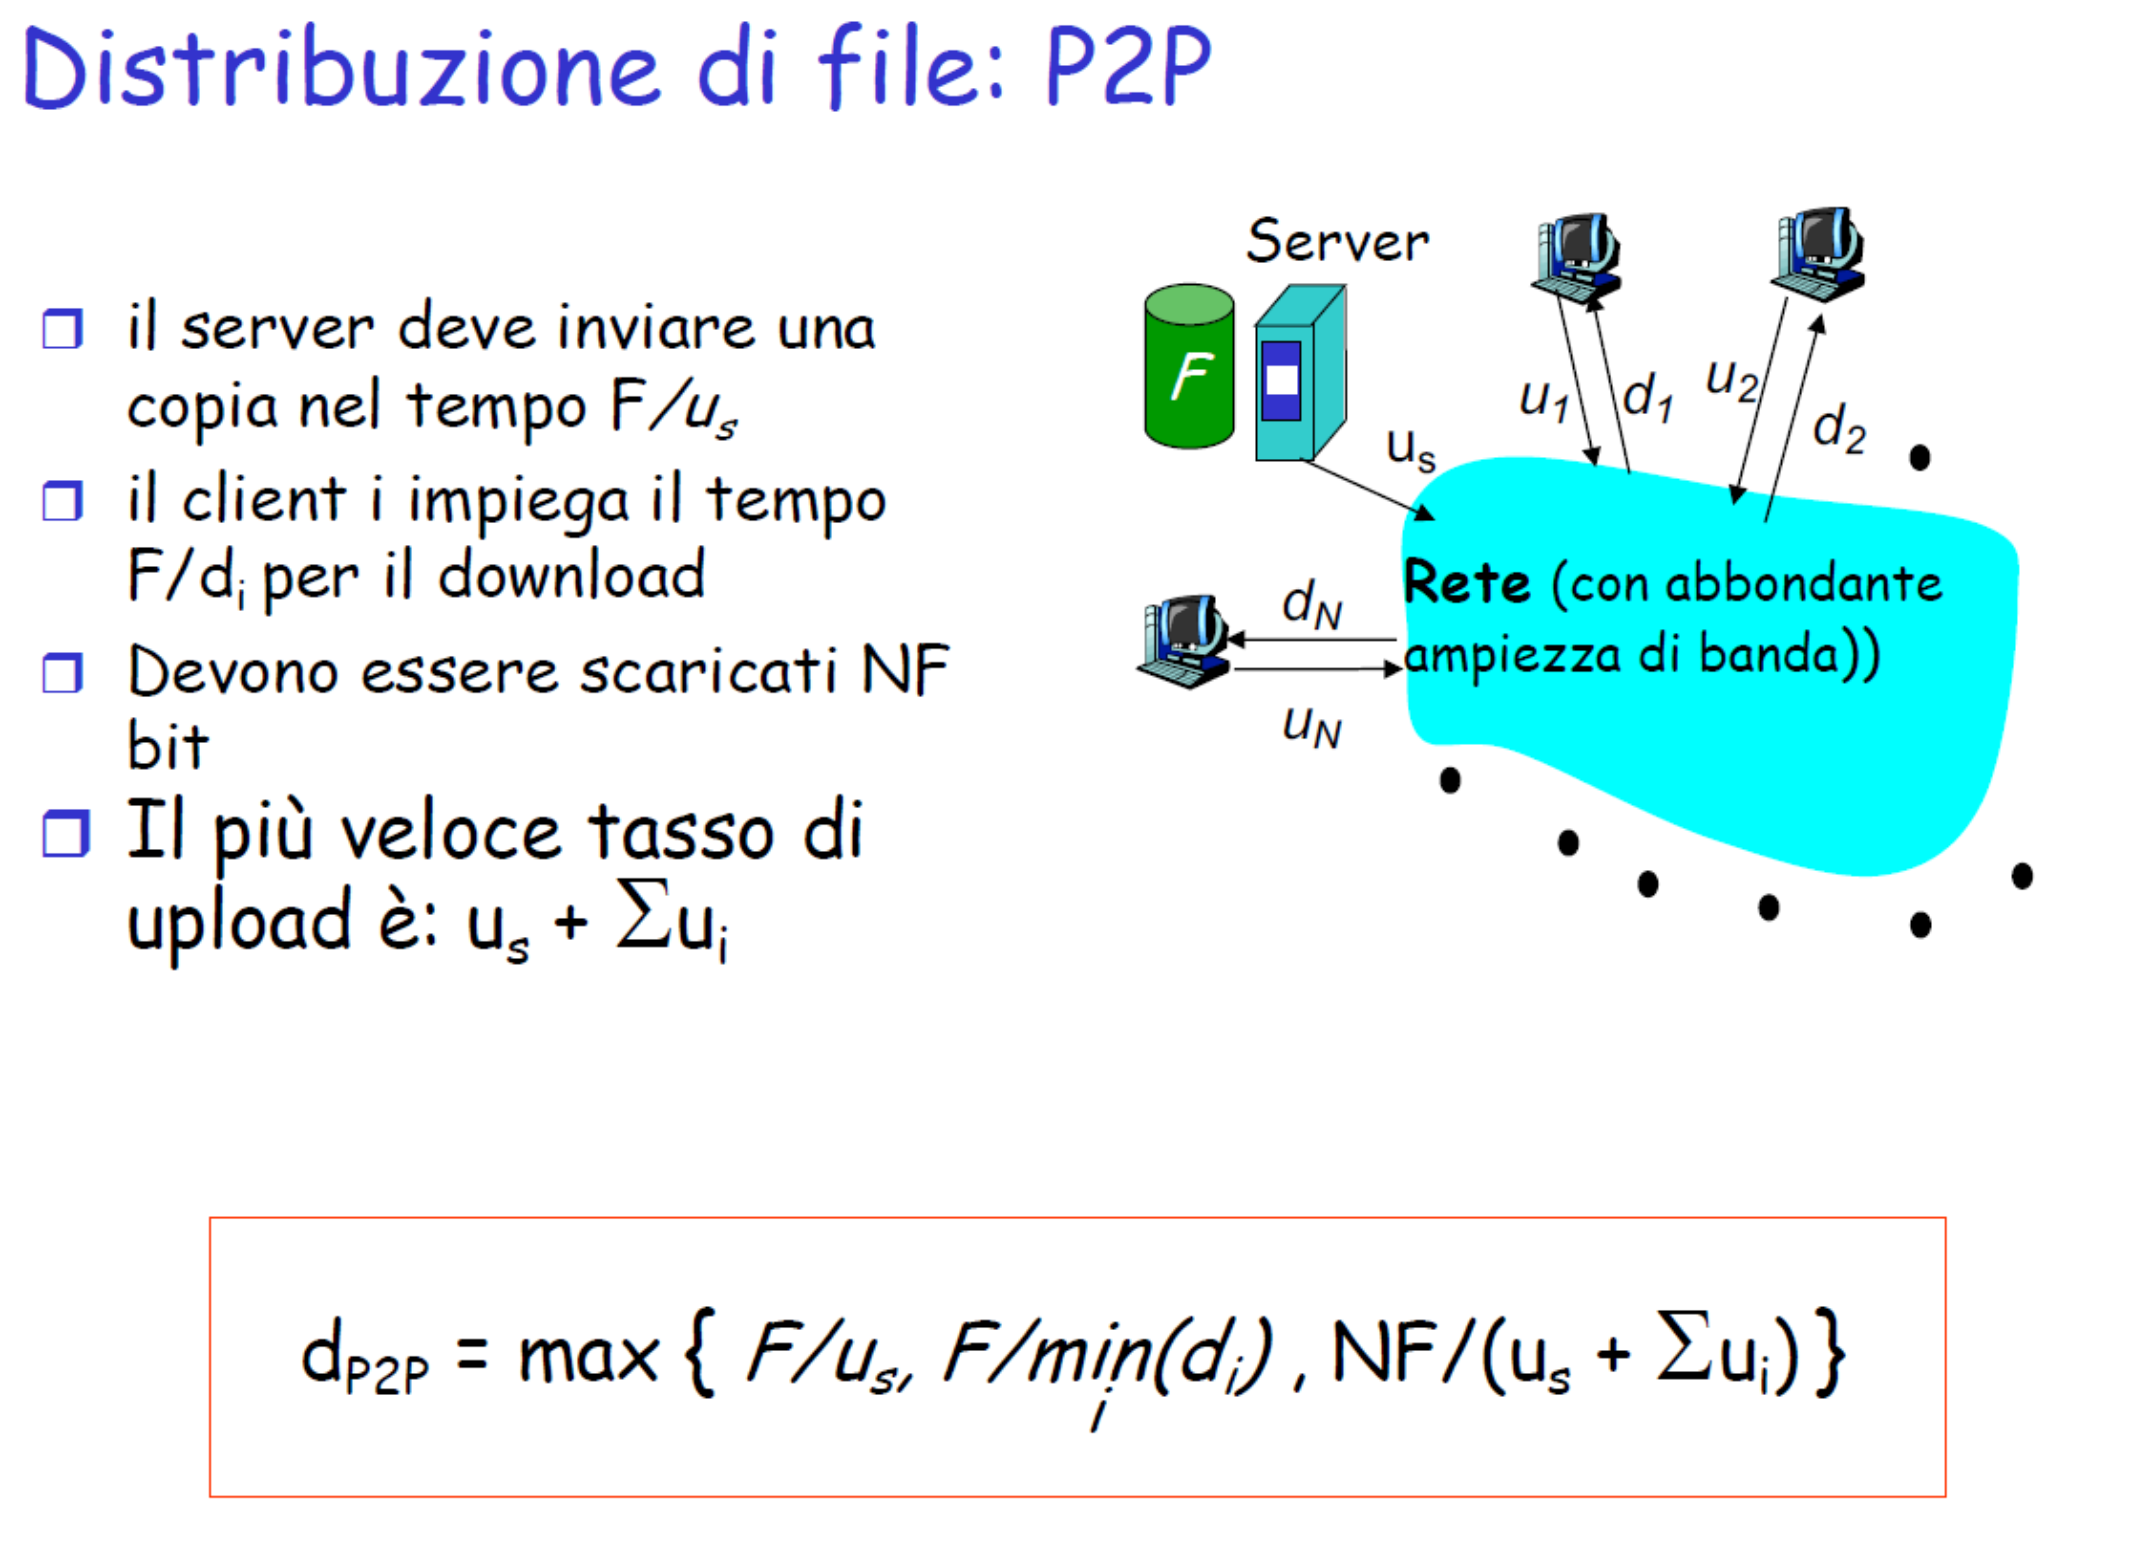
\includegraphics[width=0.7\linewidth]{p2p.png}
	\end{center}
	\paragraph{Tracker} Il tracker tiene traccia dei peer che partecipano alla rete, dove un torrent è un gruppo di peer che si cambiano parti di un file.
	\medskip\\Un file condiviso è diviso in più parti da 256 Kb, chiamati \textit{chunk}. Il peer invia le sue parti a 4 vicini, quelli che gli stanno inviando alla frequenza più alta (aggiornata ogni 10 secondi). Successivamente, ogni 30 secondi viene scelto un peer a caso che riceve i chunk; oltre a questi 5 gli altri peer non riceveranno nulla.
	\paragraph{Query flooding} Ciascun peer indicizza i file che rende disponibili per la condivisione. Il messaggio di richiesta è trasmesso sulle connessioni TCP esistenti, il peer inoltra la richiesta e il messaggio di successo più trasmesso viene inviato sul percorso inverso.
	\section{Cloud Computing}
	L'architettura del cloud computing prevede uno o più server reali, generalmente in architettura ad alta affidabilità e fisicamente collocati presso i datacenter del fornitore del servizio.
	\subsection{CDN}
	Le CDN, o Content Delivery Networks, rappresentano una soluzione comune per la realizzazione di servizi su internet, la quale costruisce una rete "overlay" per la distribuzione di contenuti. Serve per memorizzare i dati il più vicino possibile ai consumatori in modo da ottimizzare le prestazioni di rete, ridurre la latenza ed evitare colli di bottiglia.
	\chapter{Il livello di Trasporto}
	\section{Servizi a livello di trasporto}
	I servizi a livello di trasporto forniscono la comunicazione logica tra processi applicativi di host differenti. I protocolli di trasporto vengono eseguiti nei sistemi terminali: il lato invio scinde i messaggi in segmenti e li passa al livello di rete, il lato ricezione invece riassembla i segmenti in messaggi e li passa al livello applicazione.
	\begin{itemize}
		\item \textbf{Livello di rete:} si occupa della comunicazione logica tra host
		\item \textbf{Livello di trasporto:} si occupa della comunicazione logica tra processi, si basa sui servizi del livello di rete e li potenzia
	\end{itemize}
	\paragraph{Demultiplexing} Nell'host ricevente, si occupa di consegnare i segmenti ricevuti alla socket appropriata.
	\paragraph{Multiplexing} Nell'host mittente, raccoglie i dati da varie socket, li incapsula con l'intestazione (usata poi nel demultiplexing).
	\newline
	\begin{wrapfigure}{r}{0.3\textwidth}
		\centering
		\vspace{-20pt}
		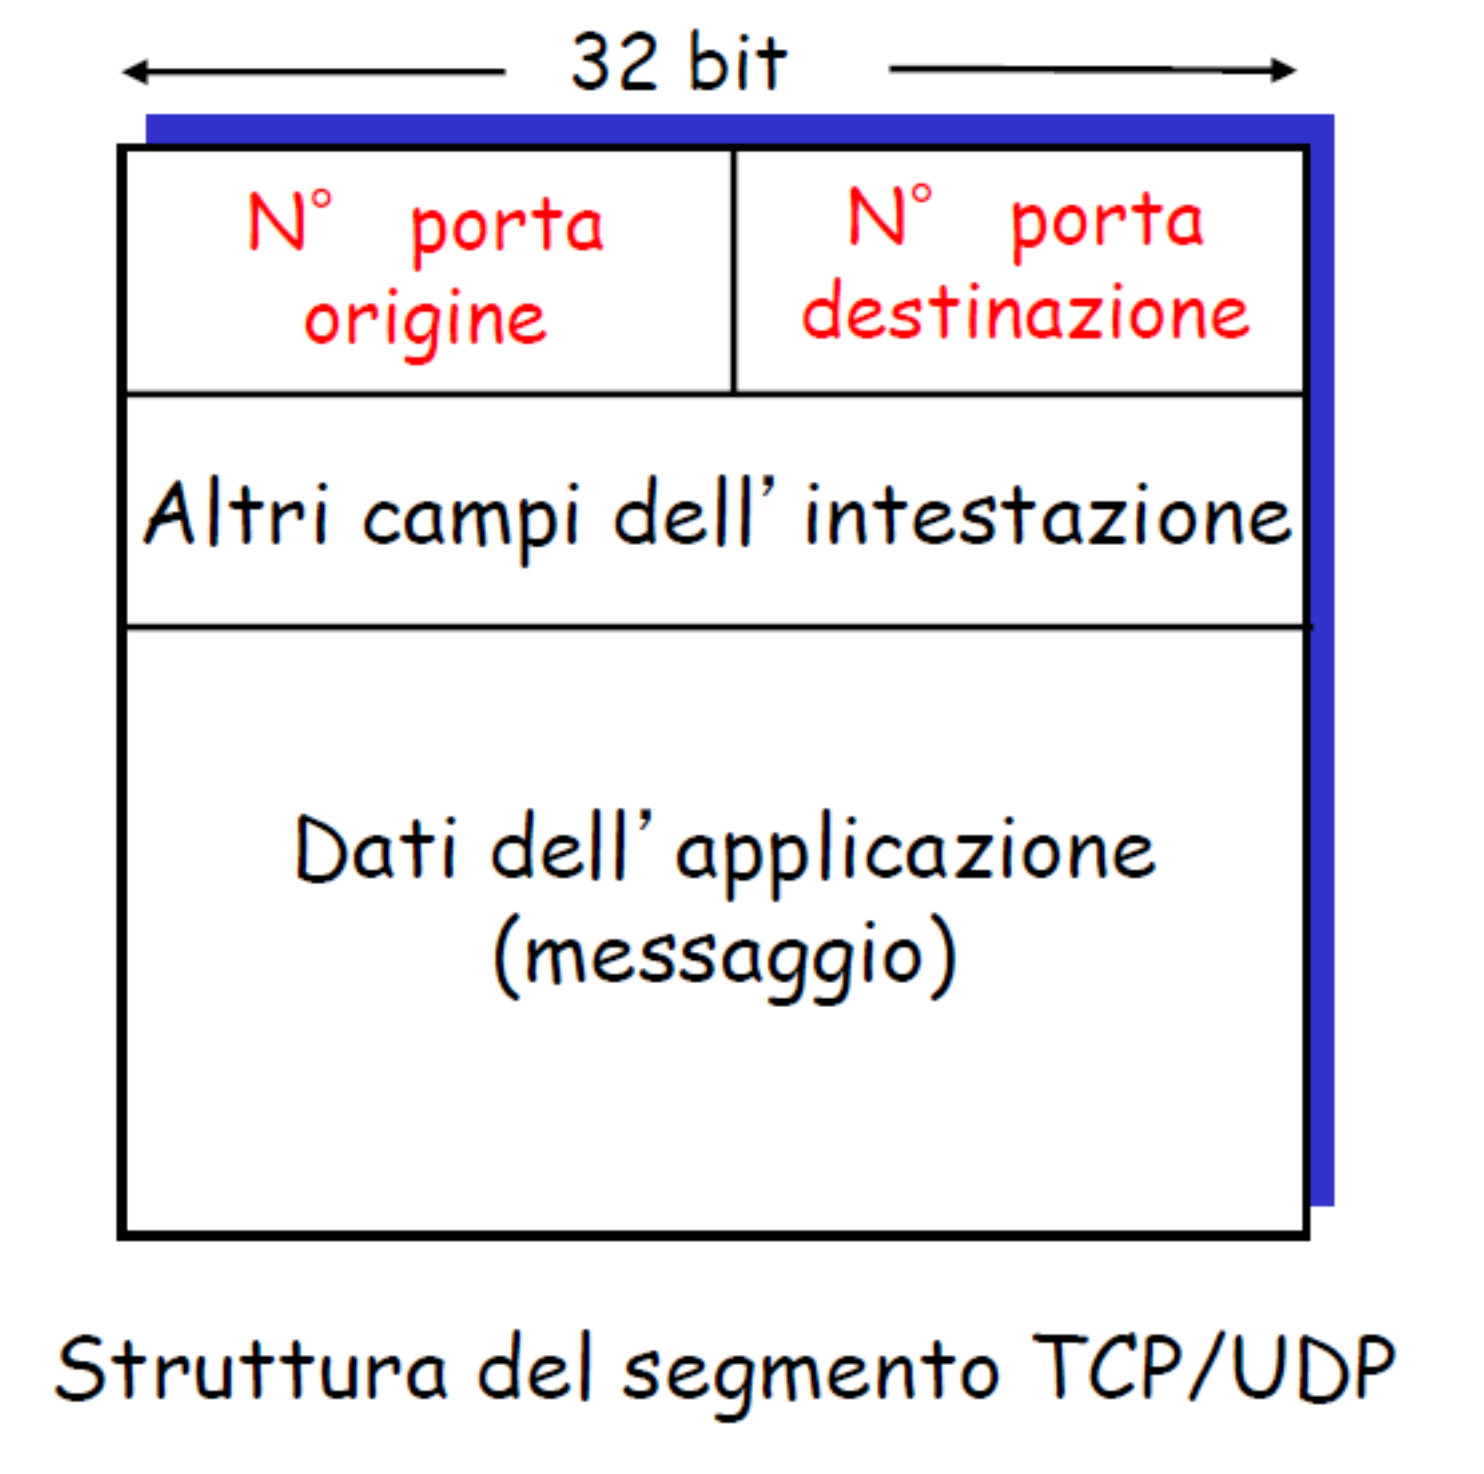
\includegraphics[width=0.25\textwidth]{segmento-trasporto}
		\vspace{-30pt}
	\end{wrapfigure}
	L’host riceve i datagrammi IP; ogni datagramma ha un indirizzo IP di origine e uno di destinazione, e trasporta 1 segmento a livello di trasporto, ogni segmento ha un numero di porta di origine e un numero di porta di destinazione. L’host usa gli indirizzi IP e i numeri di porta per inviare il segmento alla socket appropriata.
	
	\subsection{Demultiplexing senza connessione}
	Il demultiplexing senza connessione utilizza una socket UDP identificata da indirizzo IP di destinazione e numero della porta di destinazione. Quando l'host riceve il segmento UDP controlla il numero di porta nel segmento e poi lo invia alla socket correlata. Datagram IP con indirizzi IP e/o numeri di porta di origine differenti vengono inviati alla stessa socket.
	\begin{center}
		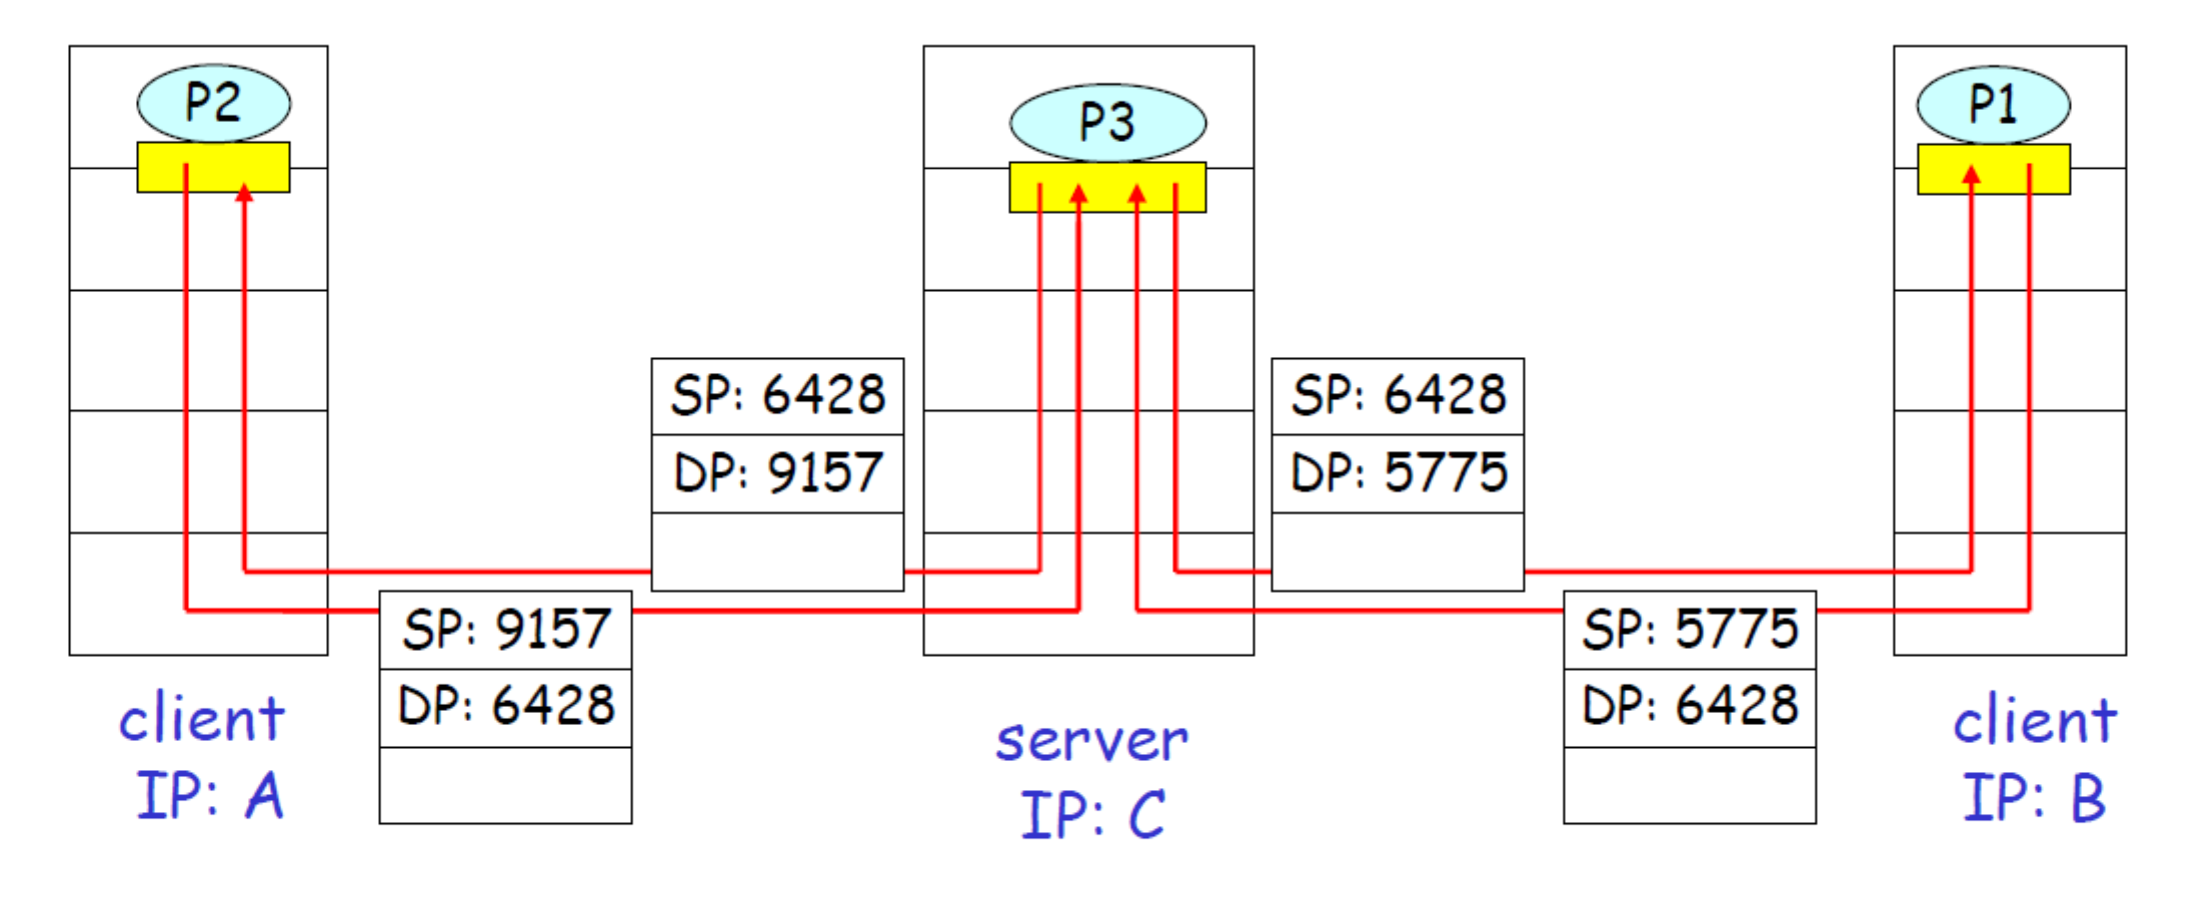
\includegraphics[width=0.7\linewidth]{socket-udp}
		\text{Demultiplexing senza connessione}
	\end{center}
	\subsection{Demultiplexing orientato alla connessione}
	Il demultiplexing orientato alla connessione utilizza una socket TCP identificata da quattro parametri: indirizzo IP e porta d'origine e indirizzo IP e porta di destinazione. L'host ricevente usa tutti e quattro i parametri per inviare il segmento alla socket appropriata. Un host server può supportare più socket TCP contemporanee. I server web hanno socket differenti per ogni connessione client, con HTTP non-persistente si avrà invece una socket differente per ogni richiesta.
	\begin{center}
		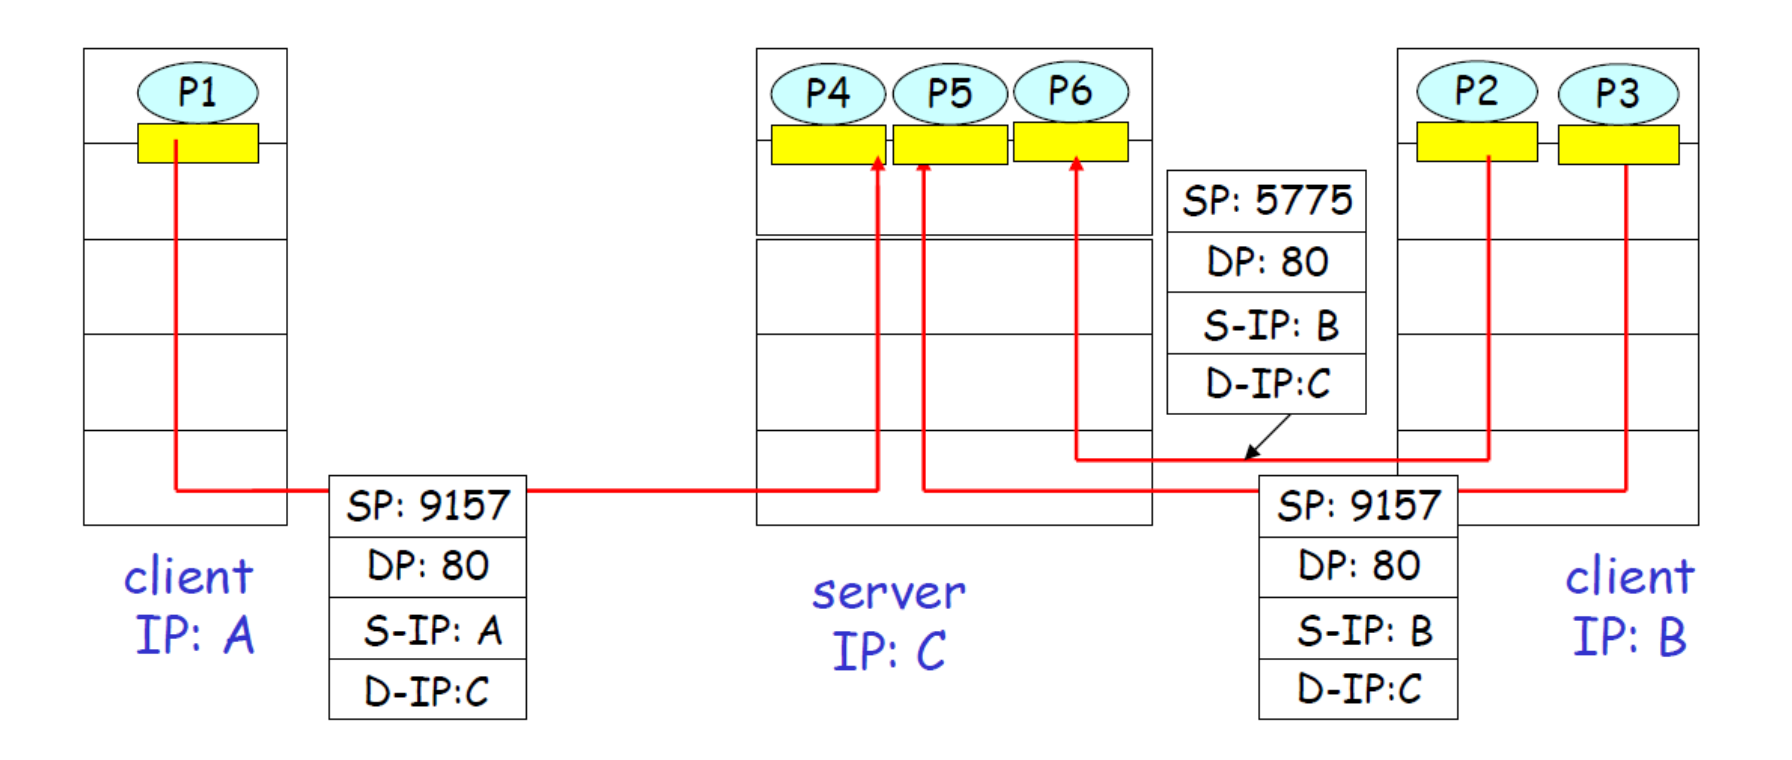
\includegraphics[width=0.7\linewidth]{socket-tcp}
	\end{center}
	\section{Trasporto senza connessione: UDP}
	\begin{wrapfigure}{r}{0.3\textwidth}
		\centering
		\vspace{-30pt}
		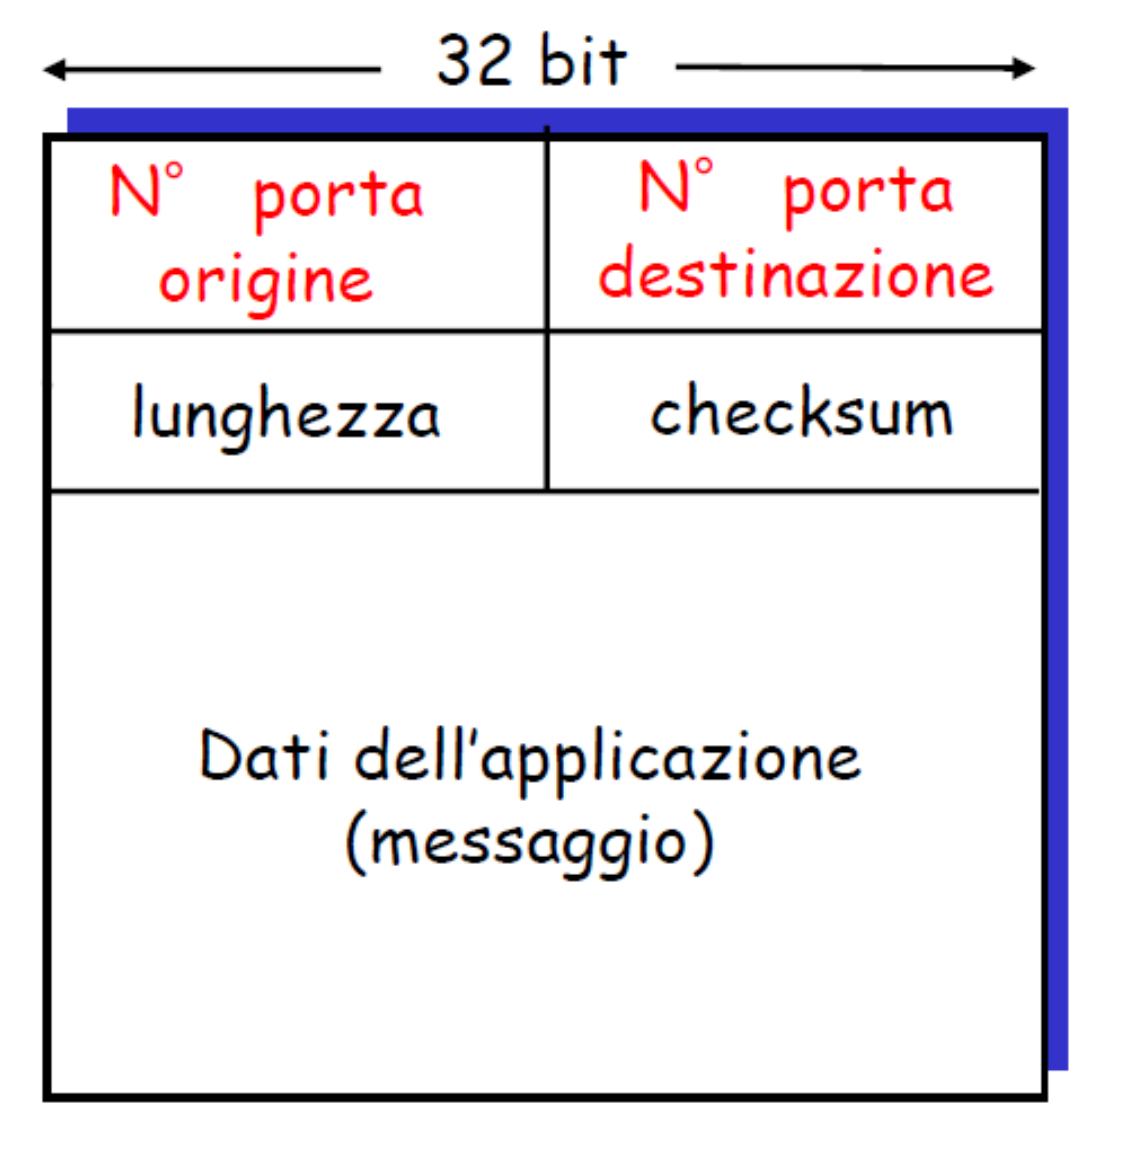
\includegraphics[width=0.25\textwidth]{segmento-udp}
		\vspace{-20pt}
	\end{wrapfigure}

	UDP, User Datagram Protocol, è un protocollo di trasporto "senza fronzoli", infatti ha un servizio di consegna best effort (miglior sforzo). Per questo i segmenti UDP possono essere perduti o consegnati fuori sequenza all'applicazione.\medskip\\ Essendo senza connessione non c'è handshaking tra mittente e destinatario, quindi ogni segmento UDP è gestito indipendentemente dagli altri.
	\paragraph{Checksum UDP} Il checksum UDP serve per rilevare gli “errori” (bit alternati) nel segmento trasmesso, il segmento viene trattato come una sequenza di interi da 16 bit.

	\section{Principi del trasferimento dati affidabile}
	\begin{center}
		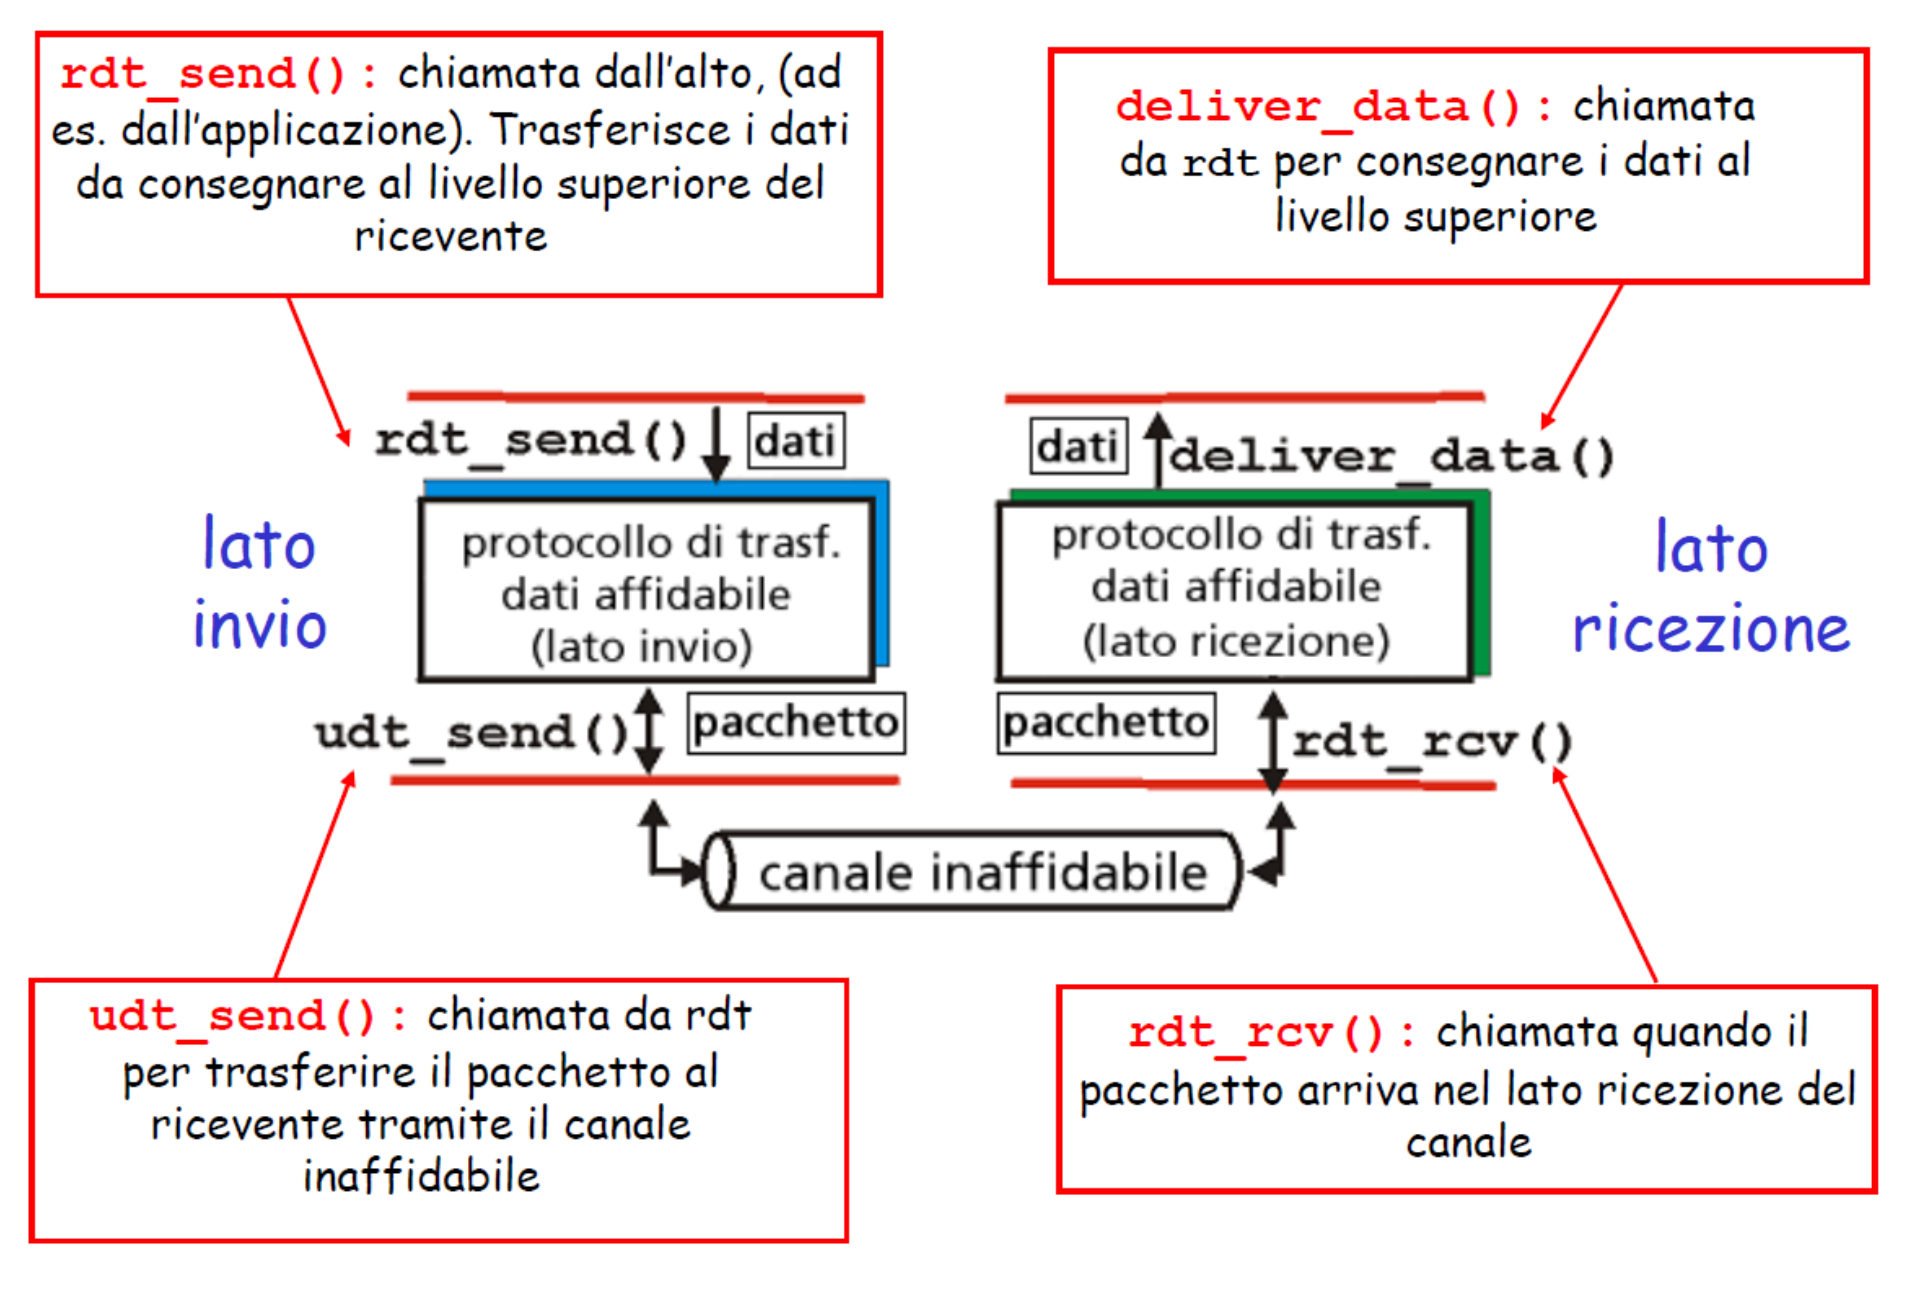
\includegraphics[width=0.7\linewidth]{rdt-1}
	\end{center}
	\paragraph{Stato di Rdt} Lo stato successivo a quello corrente è determinato unicamente dall'evento successivo
	\begin{center}
		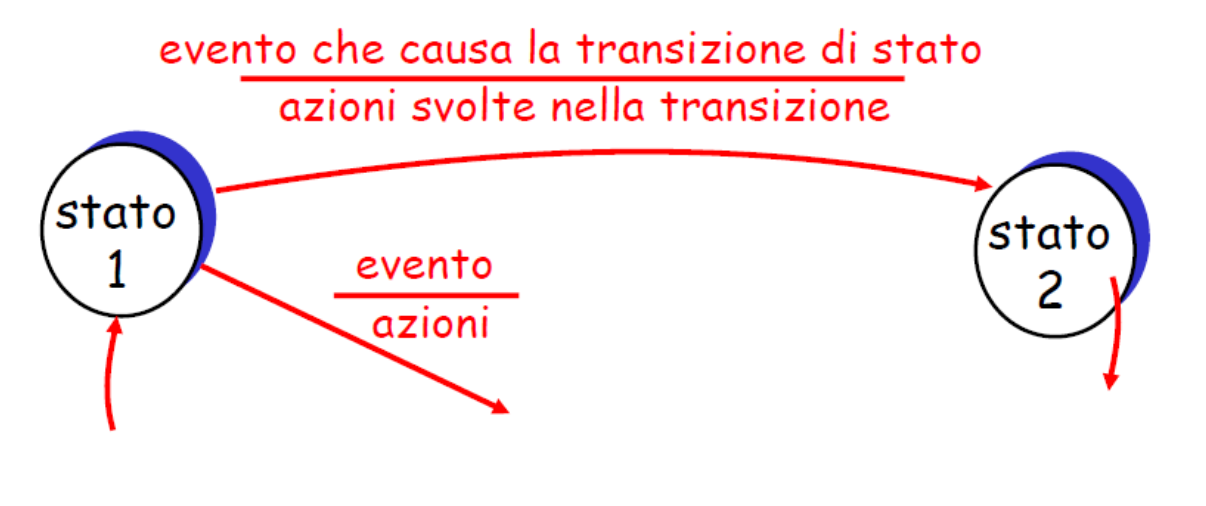
\includegraphics[width=0.7\linewidth]{rdt-stato}
	\end{center}
	\subsection{Rdt 1.0: trasferimento affidabile su canale affidabile}
	Il canale sottostante è perfettamente affidabile e è presente un automa distinto per mittente e ricevente.
	\subsection{Rdt 2.0: canale con errori nei bit}
	Il canale sottostante potrebbe confondere i bit nei pacchetti, si utilizza quindi il checksum per rilevare gli errori. Una volta ricevuto, con la notifica positiva \textbf{ACK} il ricevente comunica espressamente al mittente che il pacchetto ricevuto è corretto mentre con la notifica negativa \textbf{NAK} comunica che il pacchetto contiene errori. Se il mittente riceve un NAK verrà ritrasmesso il pacchetto.
	\medskip\\Con Rdt 2.0 sono stati introdotti nuovi meccanismi tra cui il rilevamento di errore e il feedback del destinatario (ACK e NAK).
	\medskip\\ Rdt 2.0 però ha un difetto fatale: se i pacchetti NAK e ACK sono danneggiati il mittente non saprà cos'è successo; non basta però ritrasmettere la notifica perché sono possibili duplicati.
	Il mittente ritrasmette quindi il pacchetto aggiungendo un numero di sequenza, e il ricevente lo scarterà se duplicato. Una volta inviato, il mittente aspetta la risposta del destinatario (\textit{stop and wait}).
	\subsection{Rdt 2.1}
	Il mittente aggiunge un numero di sequenza al pacchetto, saranno sufficienti due numeri (0 e 1). Dovrà poi controllare se gli ACK/NAK sono danneggiati e ricordarsi se il pacchetto corrente ha numero di sequenza 0 o 1.
	\medskip\\Il ricevente deve invece controllare se il pacchetto ricevuto è duplicato, lo stato indicherà se il numero di sequenza atteso è 0 o 1. Il ricevente non potrà però sapere se il suo ultimo ACK/NAK è stato ricevuto correttamente dal mittente.
	\subsection{Rdt 2.2: un protocollo senza NAK}
	Ha le stesse funzionalità di Rdt 2.1, utilizzando solamente gli ACK. In sostituzione al NAK il destinatario invierà un ACK per l'ultimo pacchetto ricevuto correttamente, il destinatario invece deve includere esplicitamente il numero di sequenza con l'ACK. Un ACK duplicato presso il mittente determina la stessa azione del NAK, cioè ritrasmettere il pacchetto corrente.
	 \subsection{Rdt 3.0: canali con errori e perdite}
	 Può succedere che il canale sottostante smarrisca i pacchetti (dati o ACK). Per ovviare a ciò il mittente attende un ACK per un tempo ragionevole, dopodiché, se non ricevuto, ritrasmetterà il pacchetto.
	 \medskip\\Se il pacchetto (o l'ACK) è solo in ritardo la trasmissione sarà duplicata, ma il problema è già gestita dai numeri di sequenza, che il destinatario specificherà anche nei pacchetti da riscontrare; è necessaria l'introduzione di un contatore.
	\begin{center}
		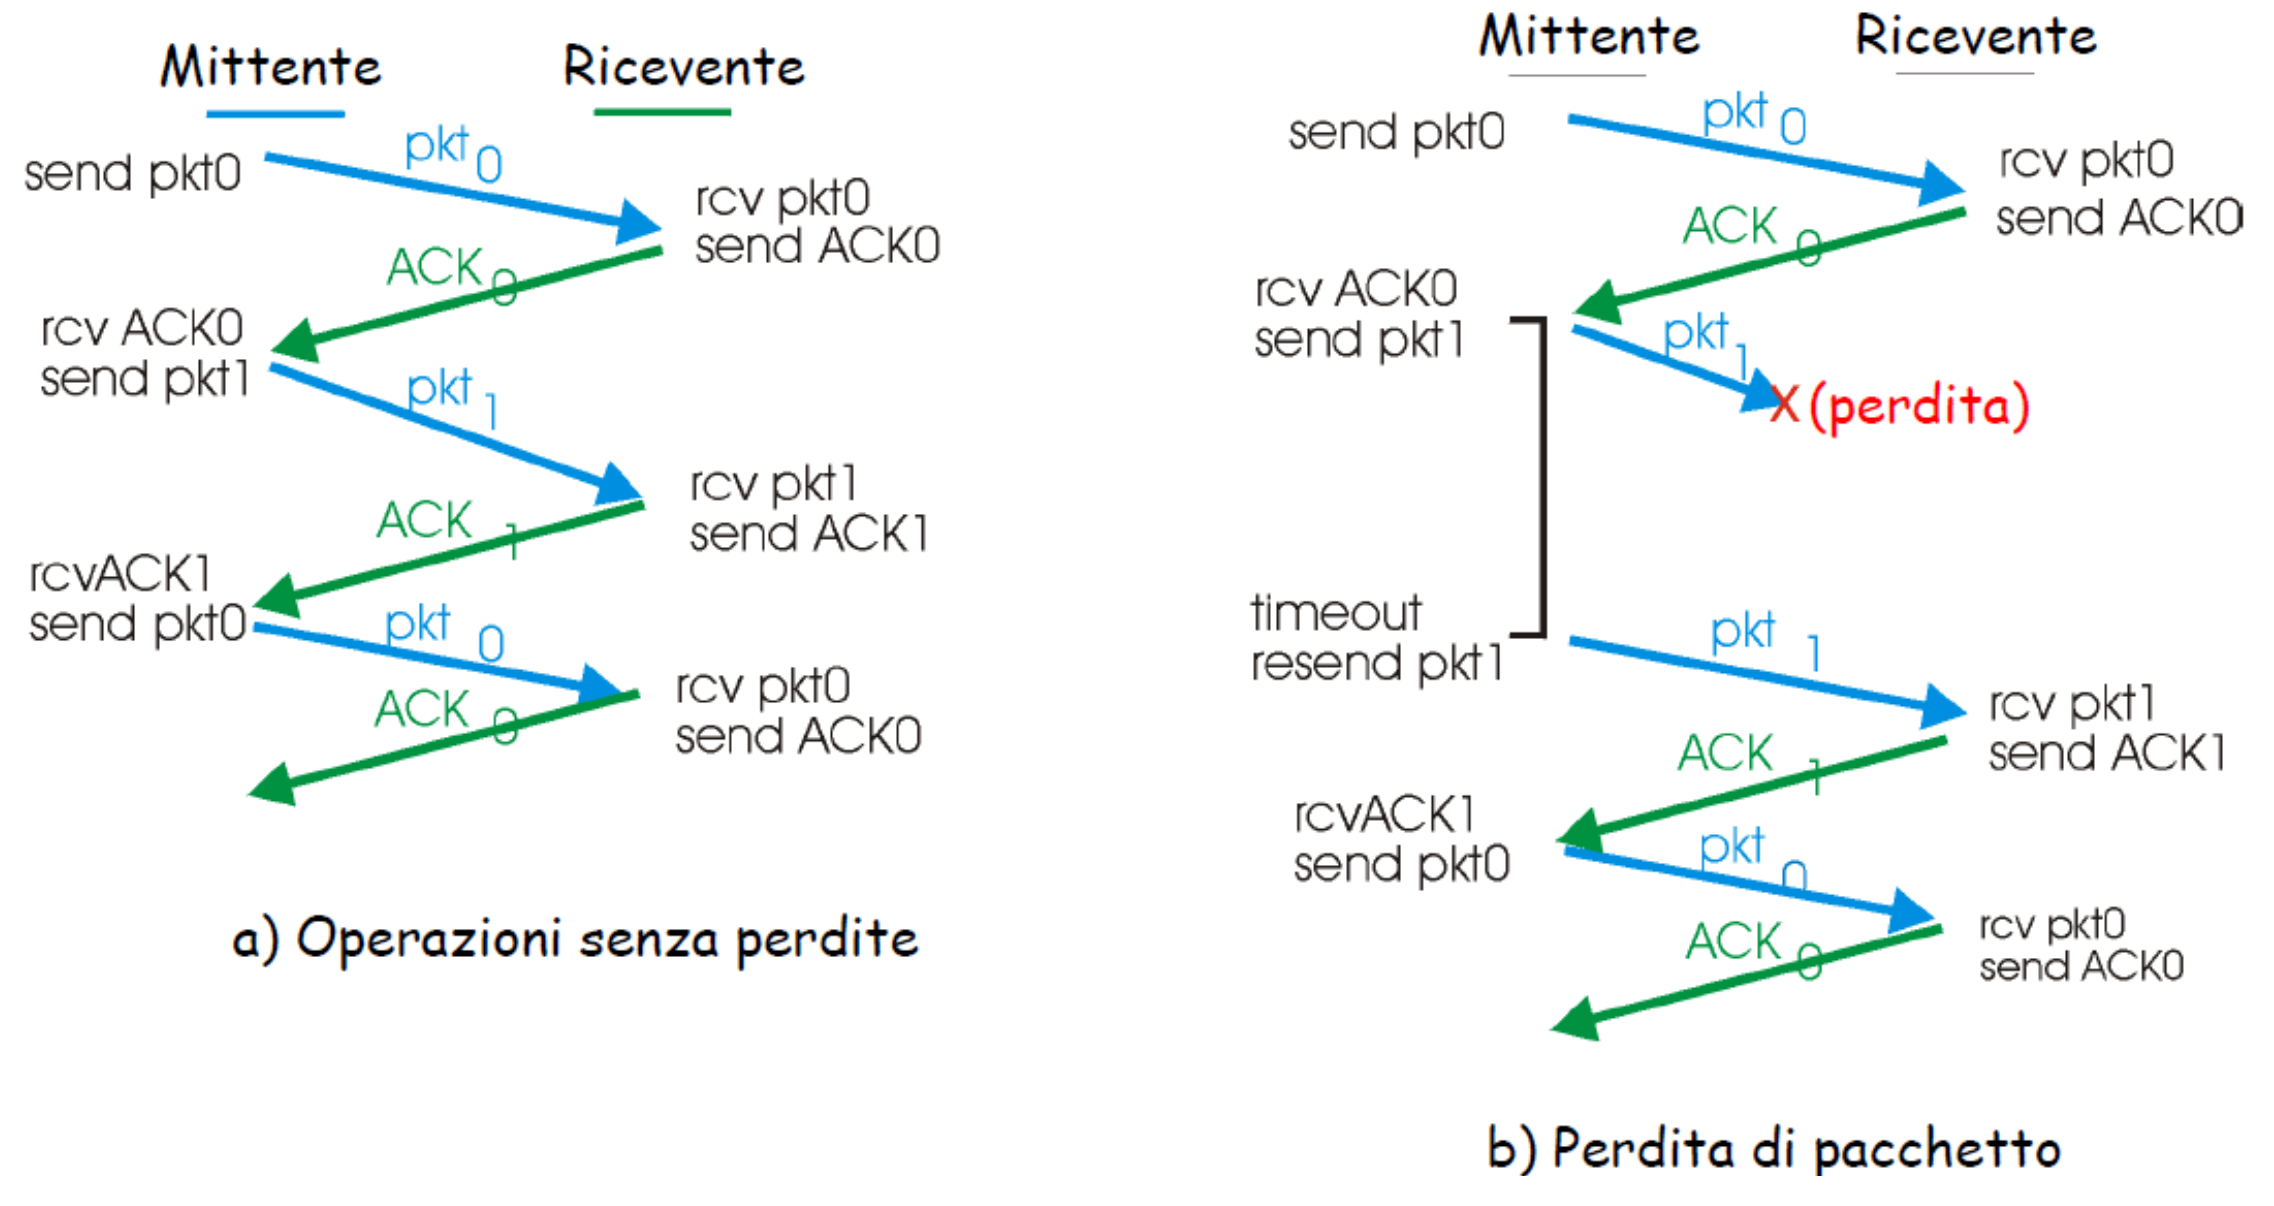
\includegraphics[width=0.7\linewidth]{rdt-2}
		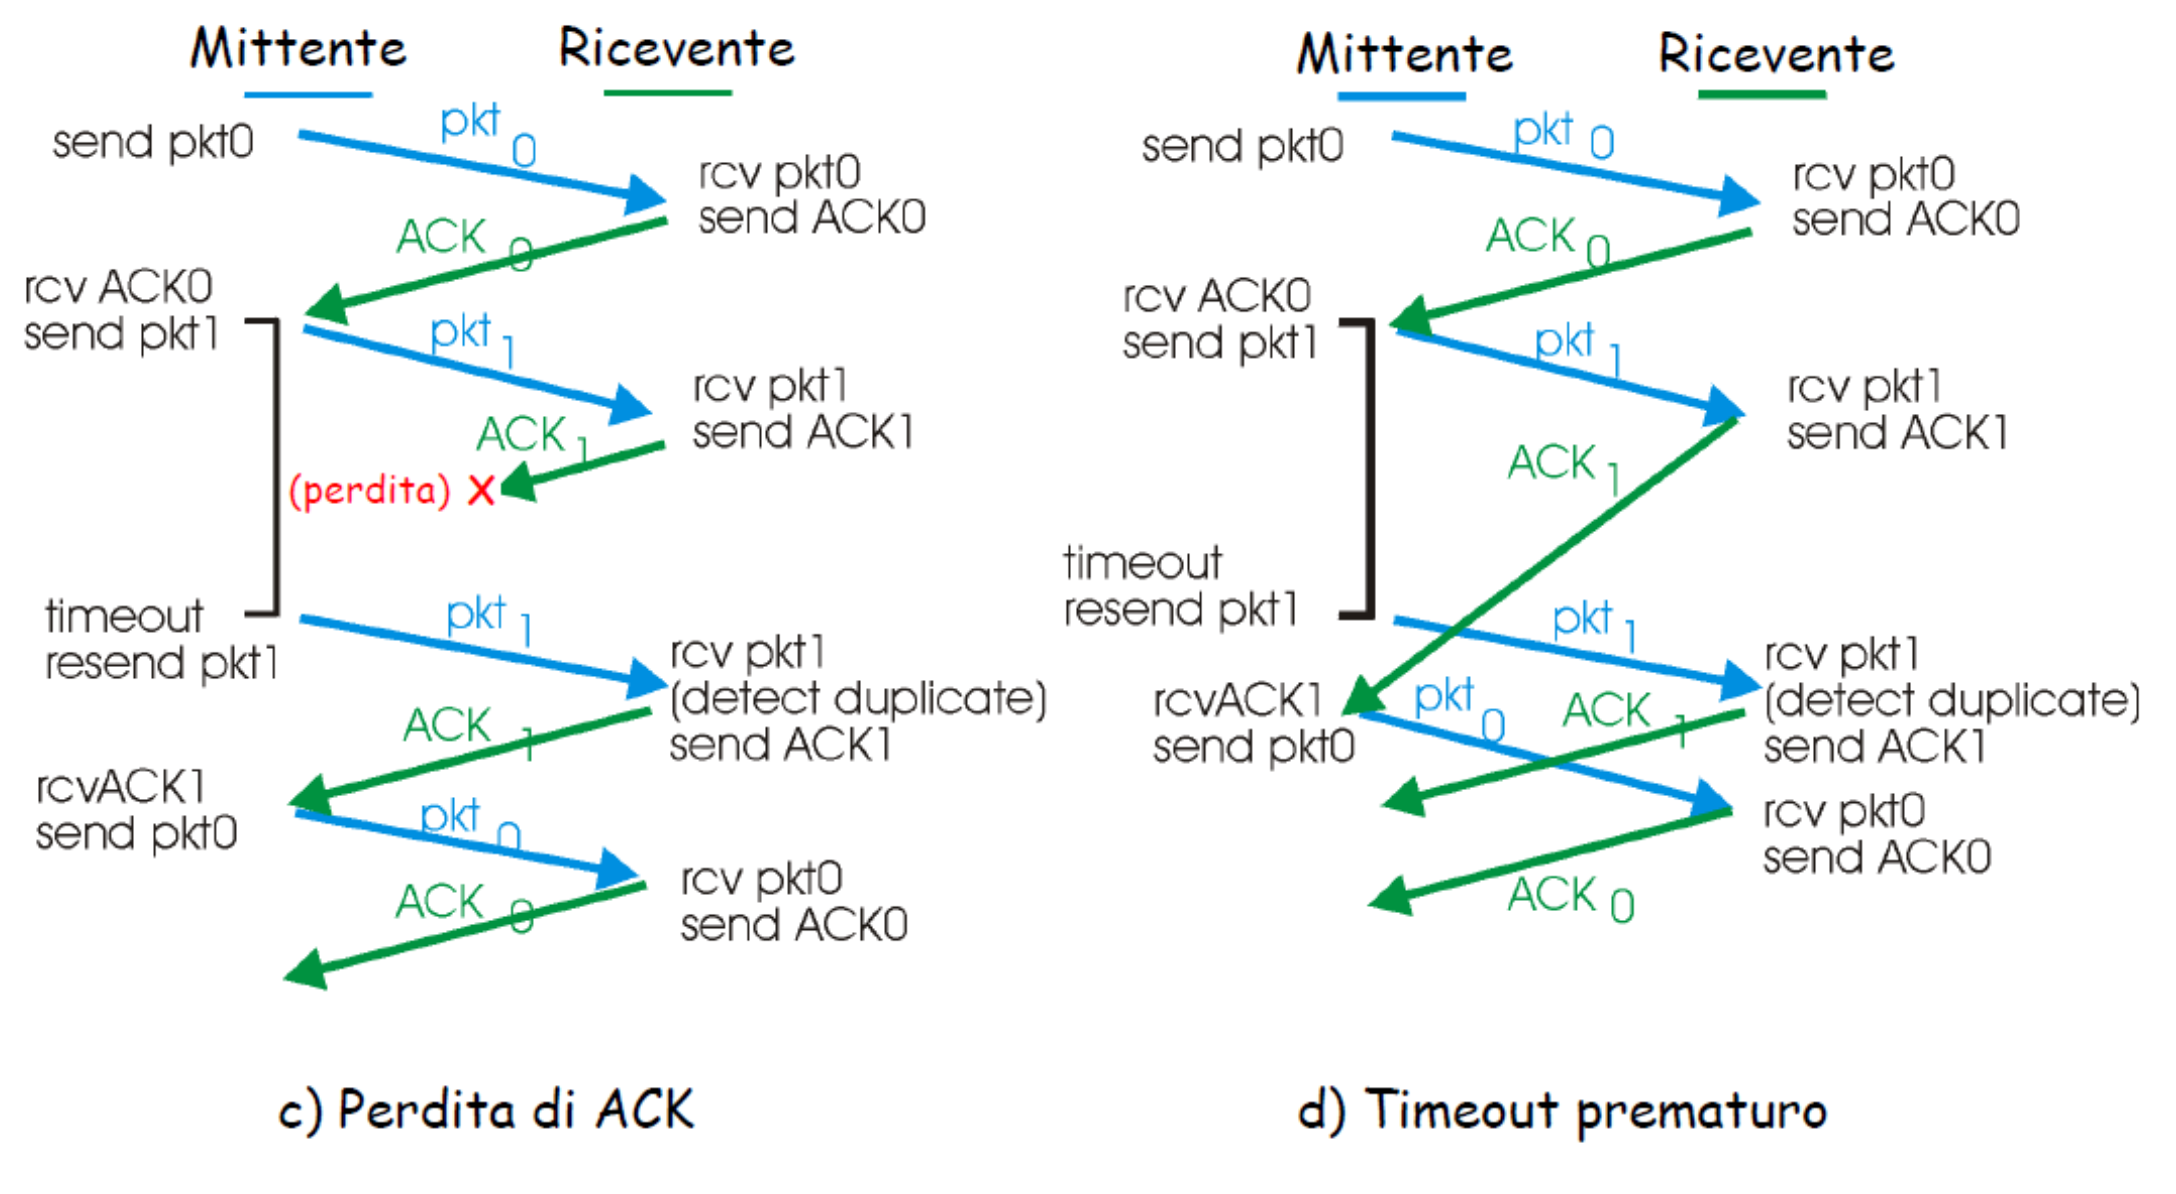
\includegraphics[width=0.7\linewidth]{rdt-3}
	\end{center}
	\subsection{Pipelining} Il mittente ammette più pacchetti in transito ancora da notificare, il loro numero di sequenza deve essere incrementale ed è presente un buffering dei pacchetti presso il mittente e il ricevente. Ci sono due forme generiche di protocolli con pipeline: \textit{Go-Back-N} e \textit{Ripetizione selettiva}.
	\subsubsection{Go-Back-N}
	\begin{itemize}
		\item Il mittente può avere fino a N pacchetti senza ACK in pipeline
		\item Il ricevente invia solo ACK cumulativi, non dà quindi l'ACK di un pacchetto se c'è un gap
		\item Il mittente ha un timer per il pacchetto più vecchio senza ACK.
	\end{itemize}
	\subsubsection{Ripetizione selettiva}
	\begin{itemize}
		\item Il mittente può avere fino a N pacchetti senza ACK in pipeline
		\item Il ricevente trasmette gli ACK solo sui singoli pacchetti.
		\item Il mittente mantiene un timer per ciascun pacchetto che non ha ancora ricevuto un ACK, che alla scadenza farà ritrasmettere solo i pacchetti senza ACK.
		\item Il ricevente accusa la ricevuta di ciascun singolo pacchetto.
	\end{itemize}
	\section{Trasporto orientato alla connessione: TCP}
	\begin{itemize}
		\item Implementa l'\textbf{Rdt 3.0} con pipelining
		\item \textbf{Connessione punto-punto}: un mittente e un destinatario
		\item Il flusso di byte è \textbf{affidabile} e in sequenza
		\item Il \textbf{controllo di flusso e di congestione} del TCP definiscono la dimensione della finestra di \textbf{pipelining}
		\item \textbf{Full-Duplex:} il flusso dei dati è bidirezionale nella stessa connessione e viene definita la dimensione massima del segmento (\textit{MSS})
		\item \textbf{Orientato alla connessione:} l'handshaking inizializza lo stato di mittente e destinatario prima di scambiare i dati
		\item \textbf{Flusso controllato:} il mittente non sovraccarica il destinatario
	\end{itemize}
	\begin{center}
		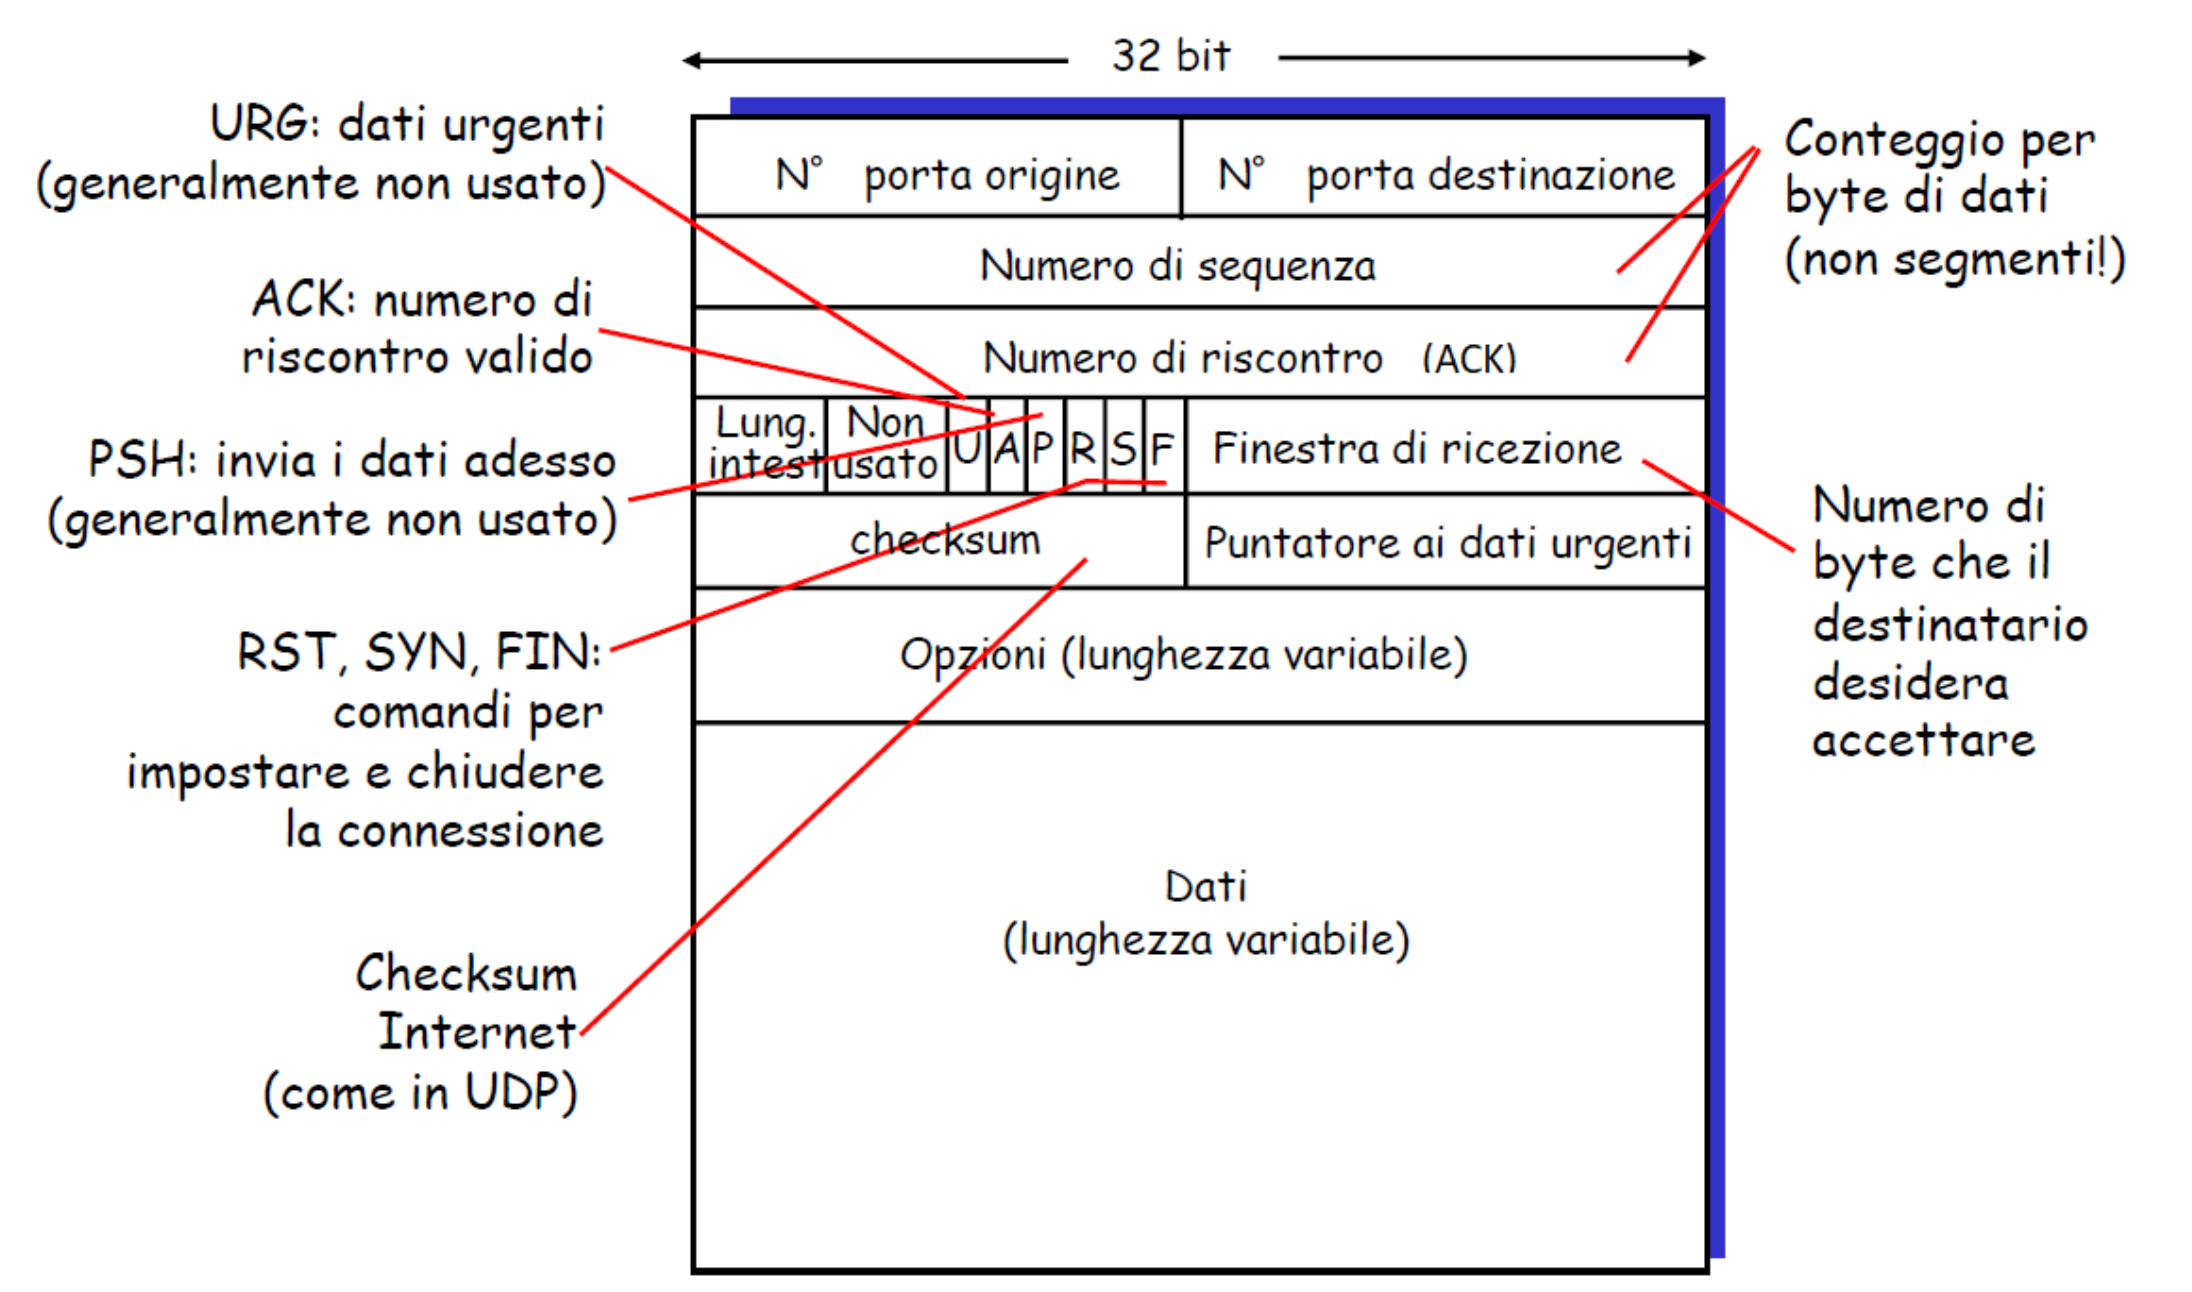
\includegraphics[width=0.7\linewidth]{segmento-tcp}
	\end{center}
	Alcuni dettagli sul segmento TCP:
	\begin{itemize}
		\item \textbf{Lunghezza dell'intestazione:} serve per sapere se ci sono informazioni nella parte opzionale, in caso negativo sarà di default 20 (5 righe \(\cdot\) 4 byte = 20)
		\item \textbf{Numero di sequenza:} numero del primo byte del segmento nel flusso di byte
		\item \textbf{ACK:} numero di sequenza del prossimo byte atteso
		\item Per calcolare il \textbf{timeout} si usa una media esponenziale ponderata
	\end{itemize}
	Il trasporto TCP crea un servizio di trasferimento dati affidabile sul servizio inaffidabile di IP. Le ritrasmissioni sono avviate da eventi di timeout e ACK duplicati.
	\begin{center}
		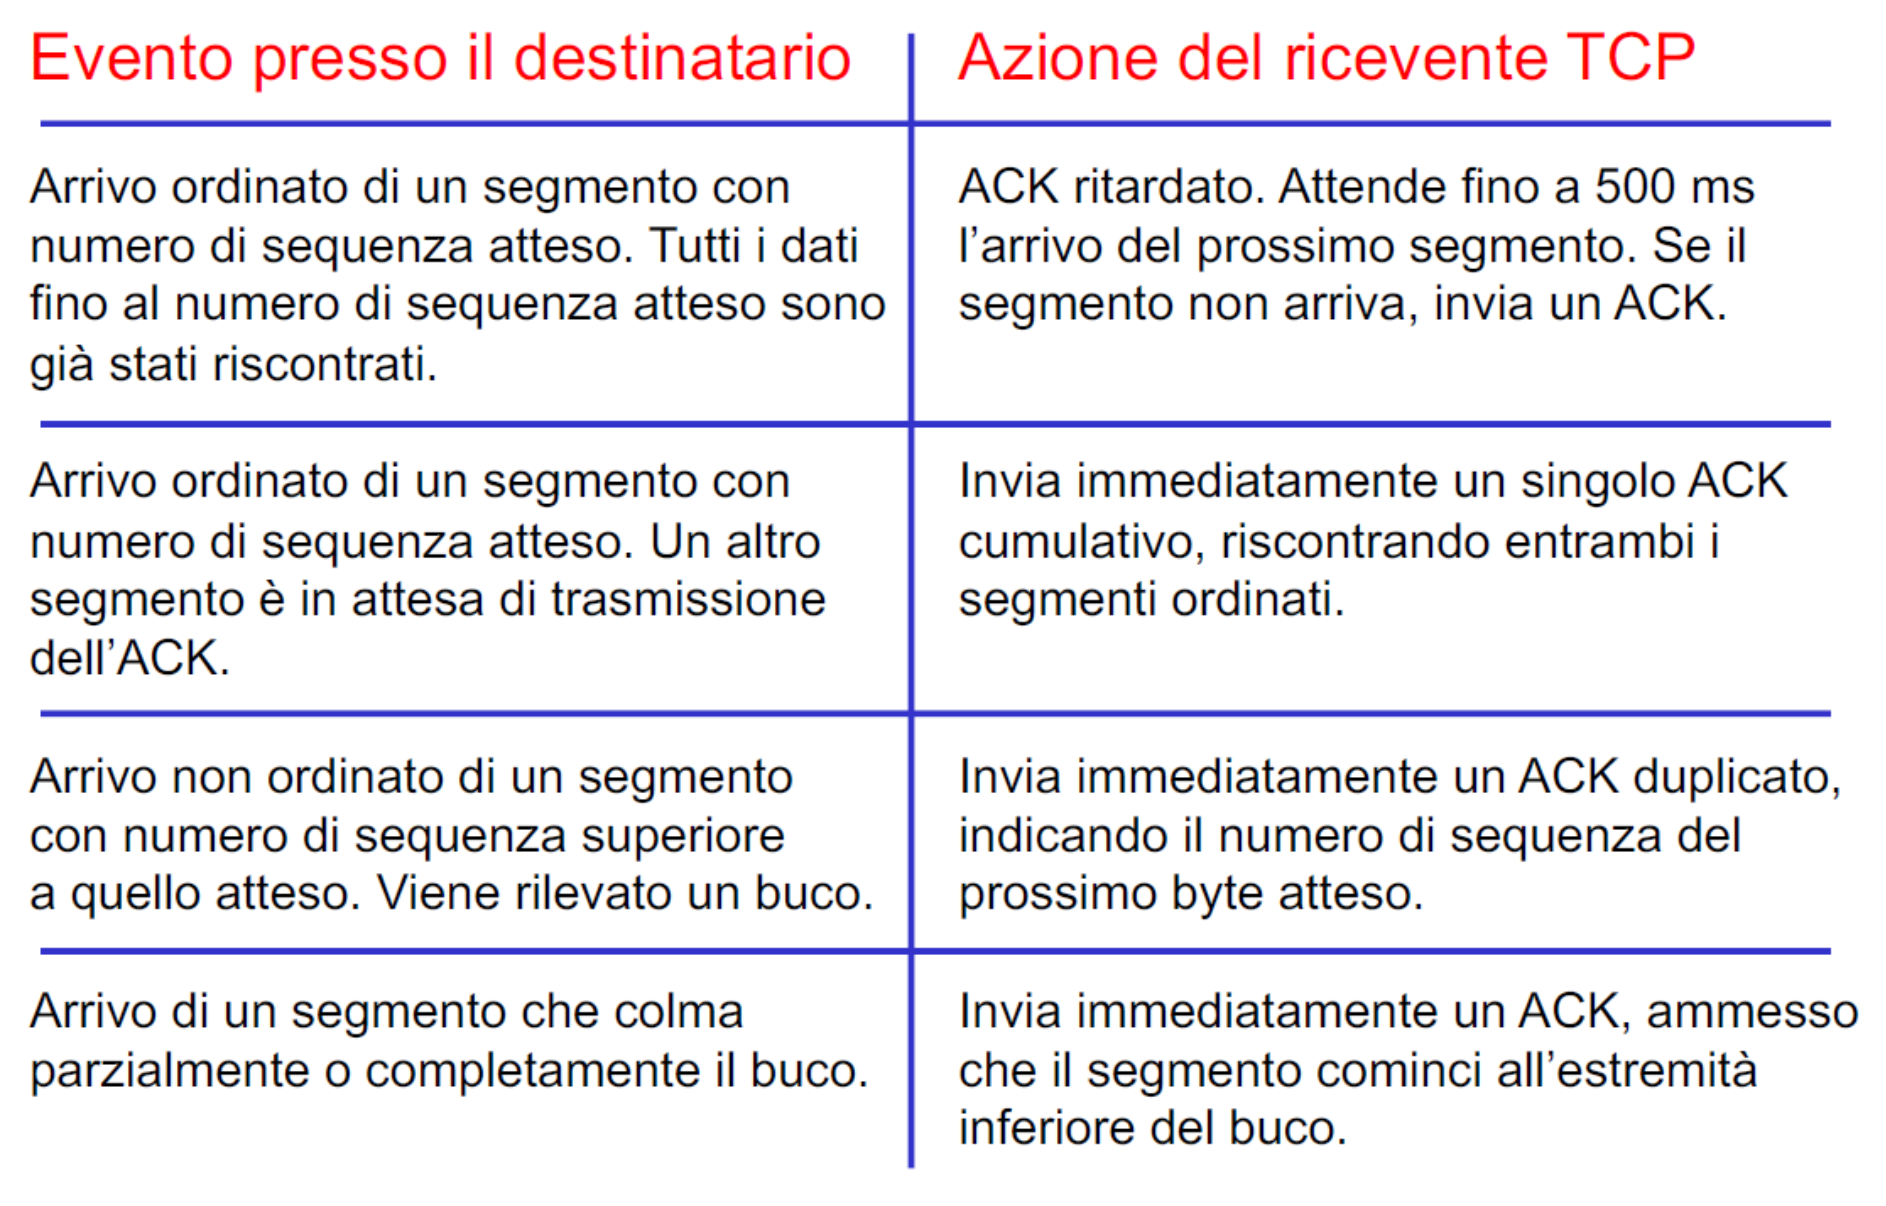
\includegraphics[width=0.7\linewidth]{eventi-tcp}
	\end{center}
	Il timeout spesso è relativamente lungo, si ha quindi un lungo ritardo prima che venga ritrasmesso il pacchetto perduto.
	\medskip\\Gli ACK perduti vengono rilevati tramite gli ACK duplicati: il mittente spesso invia molti segmenti, se un segmento viene smarrito è probabile che ci saranno molti ACK duplicati. Se il mittente riceve 3 ACK duplicati per lo stesso dato si suppone che il segmento che segue il dato riscontrato è andato perduto e rispedirà quindi il pacchetto prima che scada il timer (metodo di \textbf{trasmissione rapida}. 
	\subsection{TCP: controllo di flusso}
	\begin{wrapfigure}{r}{0.4\textwidth}
		\centering
		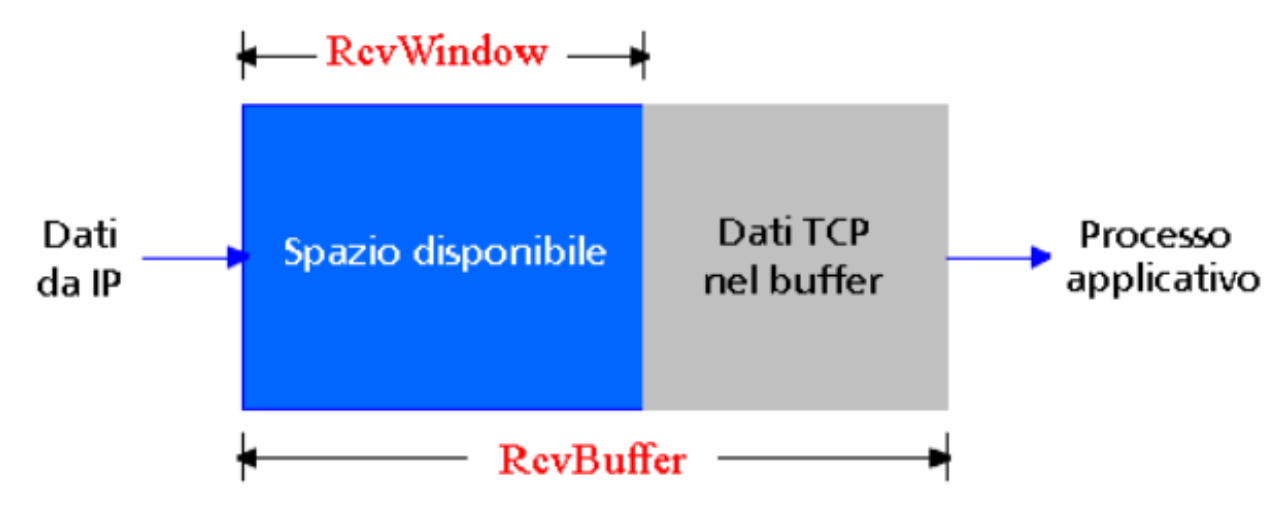
\includegraphics[width=0.4\textwidth]{controllo-di-flusso}
		\vspace{-20pt}
	\end{wrapfigure}
	
	Il lato ricevente della connessione TCP ha un buffer di ricezione, quindi il processo applicativo potrebbe essere rallentato dalla lettura del buffer. Con il controllo di flusso il mittente non vuole sovraccaricare il buffer del destinatario, trasmettendo troppi dati troppo velocemente. Il servizio di corrispondenza delle velocità indica che la frequenza di invio deve corrispondere alla frequenza di lettura dell'applicazione ricevente.
	\medskip\\Il destinatario comunica lo spazio disponibile includendo il valore \verb|RcvWindow| nei segmenti, il mittente limita i dati non riscontrati a \verb|RcvWindow| e garantisce che il buffer di ricezione non vada in overflow.
	
	\subsection{Gestione della connessione}
	La connessione viene gestita mediante un Handshake a tre vie:
	\begin{enumerate}
		\item Il client invia un segmento SYN al server che specifica il numero di sequenza iniziale, non viene inviato nessun dato
		\item Il server riceve il SYN e risponde con un segmento SYNACK e successivamente alloca i buffer
		\item Il client riceve SYNACK e risponde con un ACK che può anche contenere dati
	\end{enumerate}
	Per chiudere una connessione:
	\begin{enumerate}
		\item Il client invia un segmento di controllo FIN al server
		\item Il server riceve il segmento FIN e risponde con un ACK, chiude la connessione e invia un FIN
		\item Il client riceve il FIN e risponde con un ACK
		\item Il server riceve l'ACK e chiude la connessione
	\end{enumerate}
	
	\section{Principi del controllo di congestione}
	Per congestione si intende quando troppe sorgenti trasmettono troppi dati a una velocità talmente elevata che la rete non è in grado di gestirli. I sintomi della congestione possono essere pacchetti smarriti (causati da overflow nei buffer dei router) o lunghi ritardi (accodamento nei buffer).
	\medskip\\I due principali approcci al controllo di congestione sono:
	\begin{itemize}
		\item \textbf{Controllo di congestione punto-punto}
		\begin{itemize}
			\item Nessun supporto esplicito dalla rete
			\item La congestione è dedotta osservando le perdite e i ritardi nei sistemi terminali
			\item Metodo adottato da TCP
		\end{itemize}
		\item \textbf{Controllo di congestione assistito dalla rete}
		\begin{itemize}
			\item I router forniscono un feedback ai sistemi terminali
			\item Utilizzato un singolo bit per indicare la congestione
			\item Viene comunicata in modo esplicito al mittente la frequenza trasmissiva
		\end{itemize}
	\end{itemize}
	\section{Controllo di congestione in TCP (AIMD)}
	Il controllo di congestione in TCP viene effettuato mediante l'approccio AIMD; ovvero incremento additivo e decremento moltiplicativo.
	\medskip\\Consiste nell'aumentare il tasso trasmissivo sondando la rete fino a quando non si verifica una perdita. Secondo l'\textbf{incremento adattivo} fa aumentare la \verb|CongWin| di 1 MSS a ogni RTT in assenza di perdita, mentre secondo il \textbf{decremento moltiplicativo} riduce a metà \verb|CongWin| dopo un evento di perdita. La formula diventa quindi approssimativamente:
	\begin{displaymath}
  		\text{Frequenza d'invio = }\frac{CongWin}{RTT}\text{ byte/sec}
	\end{displaymath}
	
	\verb|CongWin| è una funzione dinamica della congestione percepita. Il mittente percepisce la congestione dopo un evento di perdita, quindi un timeout o una ricezione di 3 ACK duplicati, e riduce di conseguenza la frequenza di invio (\verb|CongWin|).
	\medskip\\Vengono utilizzati tre meccanismi: AIMD, partenza lenta e reazione agli eventi di timeout.
	\newpage
	\subsection{Partenza lenta}
	\begin{wrapfigure}{r}{0.3\textwidth}
		\centering
		\vspace{-20pt}
		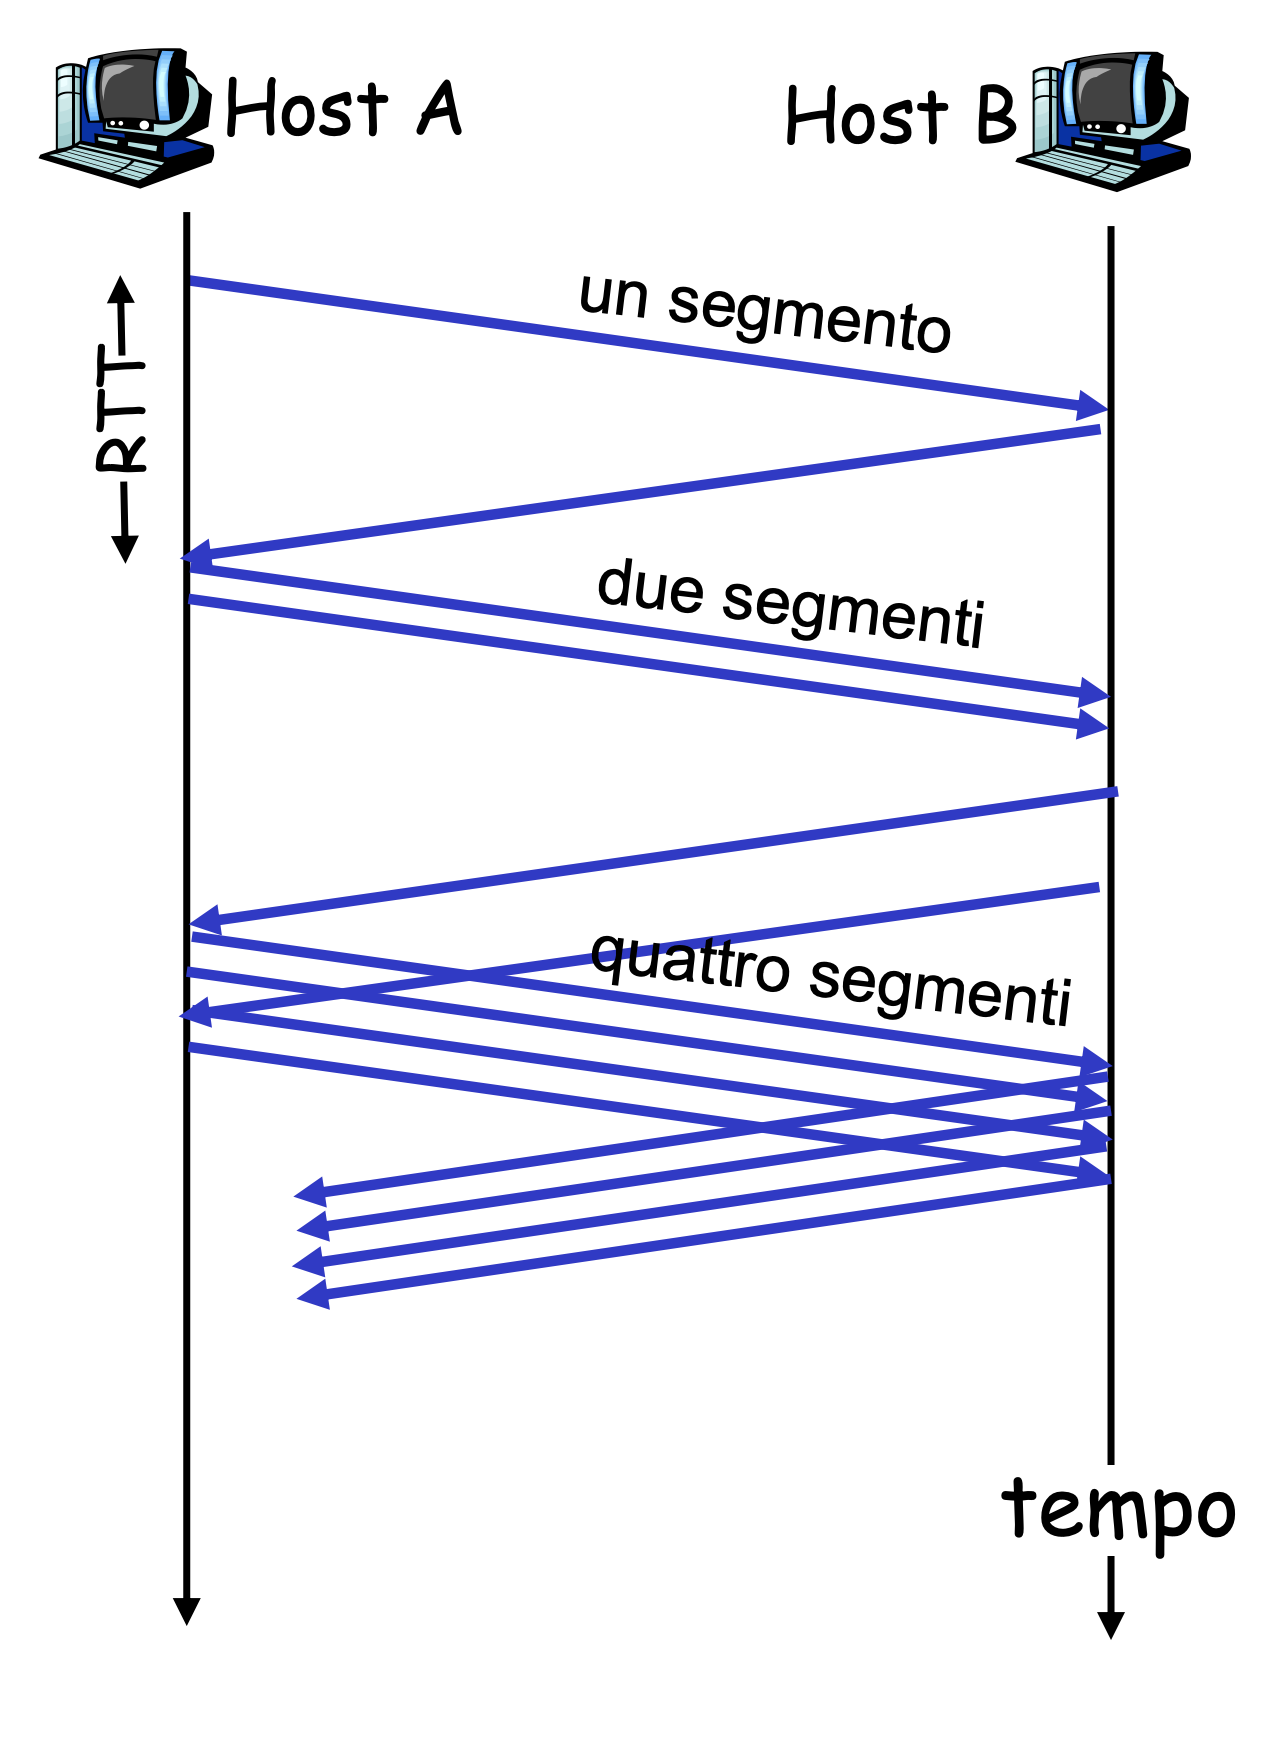
\includegraphics[width=0.3\textwidth]{partenza-lenta}
		\vspace{-50pt}
	\end{wrapfigure}
	Quando si stabilisce una connessione (\verb|CongWin| = 1 MSS) la frequenza aumenta in modo esponenziale fino a quando non si verifica una perdita: infatti \verb|CongWin| raddoppia a ogni RTT incrementandolo per ogni ACK ricevuto.
	\medskip\\Dopo 3 ACK duplicati (perdita), \verb|CongWin| è ridotto a metà e la finestra cresce linearmente. Se si verifica però un timeout, \verb|CongWin| viene impostato a 1 MSS crescendo in modo esponenziale fino a una soglia, dopo la quale crescerà linearmente.
	\medskip\\La filosofia seguita è quella che 3 ACK duplicati indicano la capacità della rete di consegnare qualche segmento, mentre un timeout prima di 3 ACK duplicati è "più allarmante".
	\medskip\\La soglia impostata è variabile, ma in caso di perdita la soglia diventa \(\frac{1}{2}\) di \verb|CongWin| appena prima dell'evento.
	\subsection{Riassunto: controllo di congestione}
	\begin{itemize}
		\item Quando \verb|CongWin| è sotto la soglia, il mittente è nella fase di \textbf{partenza lenta}; la finestra cresce in modo esponenziale.
		\item Quando \verb|CongWin| è sopra la soglia, il mittente p nella fase di \textbf{congestion avoidance}; la finestra cresce in modo lineare.
		\item Quando si verificano \textbf{tre ACK duplicati}, il valore della soglia viene impostato a \verb|CongWin/2| e \verb|CongWin| viene impostata al valore della soglia.
		\item Quando si verifica un \textbf{timeout}, il valore della soglia viene impostato a \verb|CongWin/2| e \verb|CongWin| è impostata a 1 MSS.
	\end{itemize}
	\subsection{Throughput TCP}
	Il throughput medio di TCP varia in funzione della dimensione della finestra e di RTT. Se, dopo una perdita, la finestra è W, il throughput sarà W/RTT. Dopo la perdita la finestra diventerà W/2 e il throughput di conseguenza diventa W/2RTT. Il throughput medio è quindi 0.75 W/RTT
	\subsection{Equità di TCP}
	\paragraph{Equità} se K sessioni TCP condividono lo stesso collegamento con ampiezza di banda R (collo di bottiglia), ogni sessione dovrà avere una frequenza trasmissiva media pari a R/K.
	\medskip\\TCP infatti è equo perché con due connessioni in concorrenza l'incremento additivo ha una pendenza pari a 1, mentre il decremento moltiplicativo riduce il throughput in modo proporzionale.
	\medskip\\Proprio per questo le applicazioni multimediali spesso usano UDP, poiché non vogliono che il loro tasso trasmissivo venga ridotto ma tollerano la perdita di pacchetti.
	
	\chapter{Il livello di Rete}
	
	\hypertarget{header-n0}{%
\section{Introduzione}\label{header-n0}}

\hypertarget{header-n2}{%
\subsection{Funzioni chiave del livello di rete}\label{header-n2}}

Il livello di rete svolge due funzioni principali:

\begin{itemize}
\item
  \textbf{inoltro (o forwarding):} trasferimento dei pacchetti
  dall'input di un router all'output appropriato
\item
  \textbf{instradamento (o routing):} determinare il percorso seguito
  dai pacchetti da origine a destinazione
\end{itemize}

Possiamo, per analogia, considerare l'inoltro come l'attraversamento di
uno svincolo durante un viaggio e l'instradamento come la pianificazione
dell'intero viaggio.

Per effettuare queste funzioni, viene inserito nell'header del pacchetto
un'indicazione per l'instradamento, che verrà utilizzata dal router per
fare un match con la sua tabella di routing.

\begin{center}
		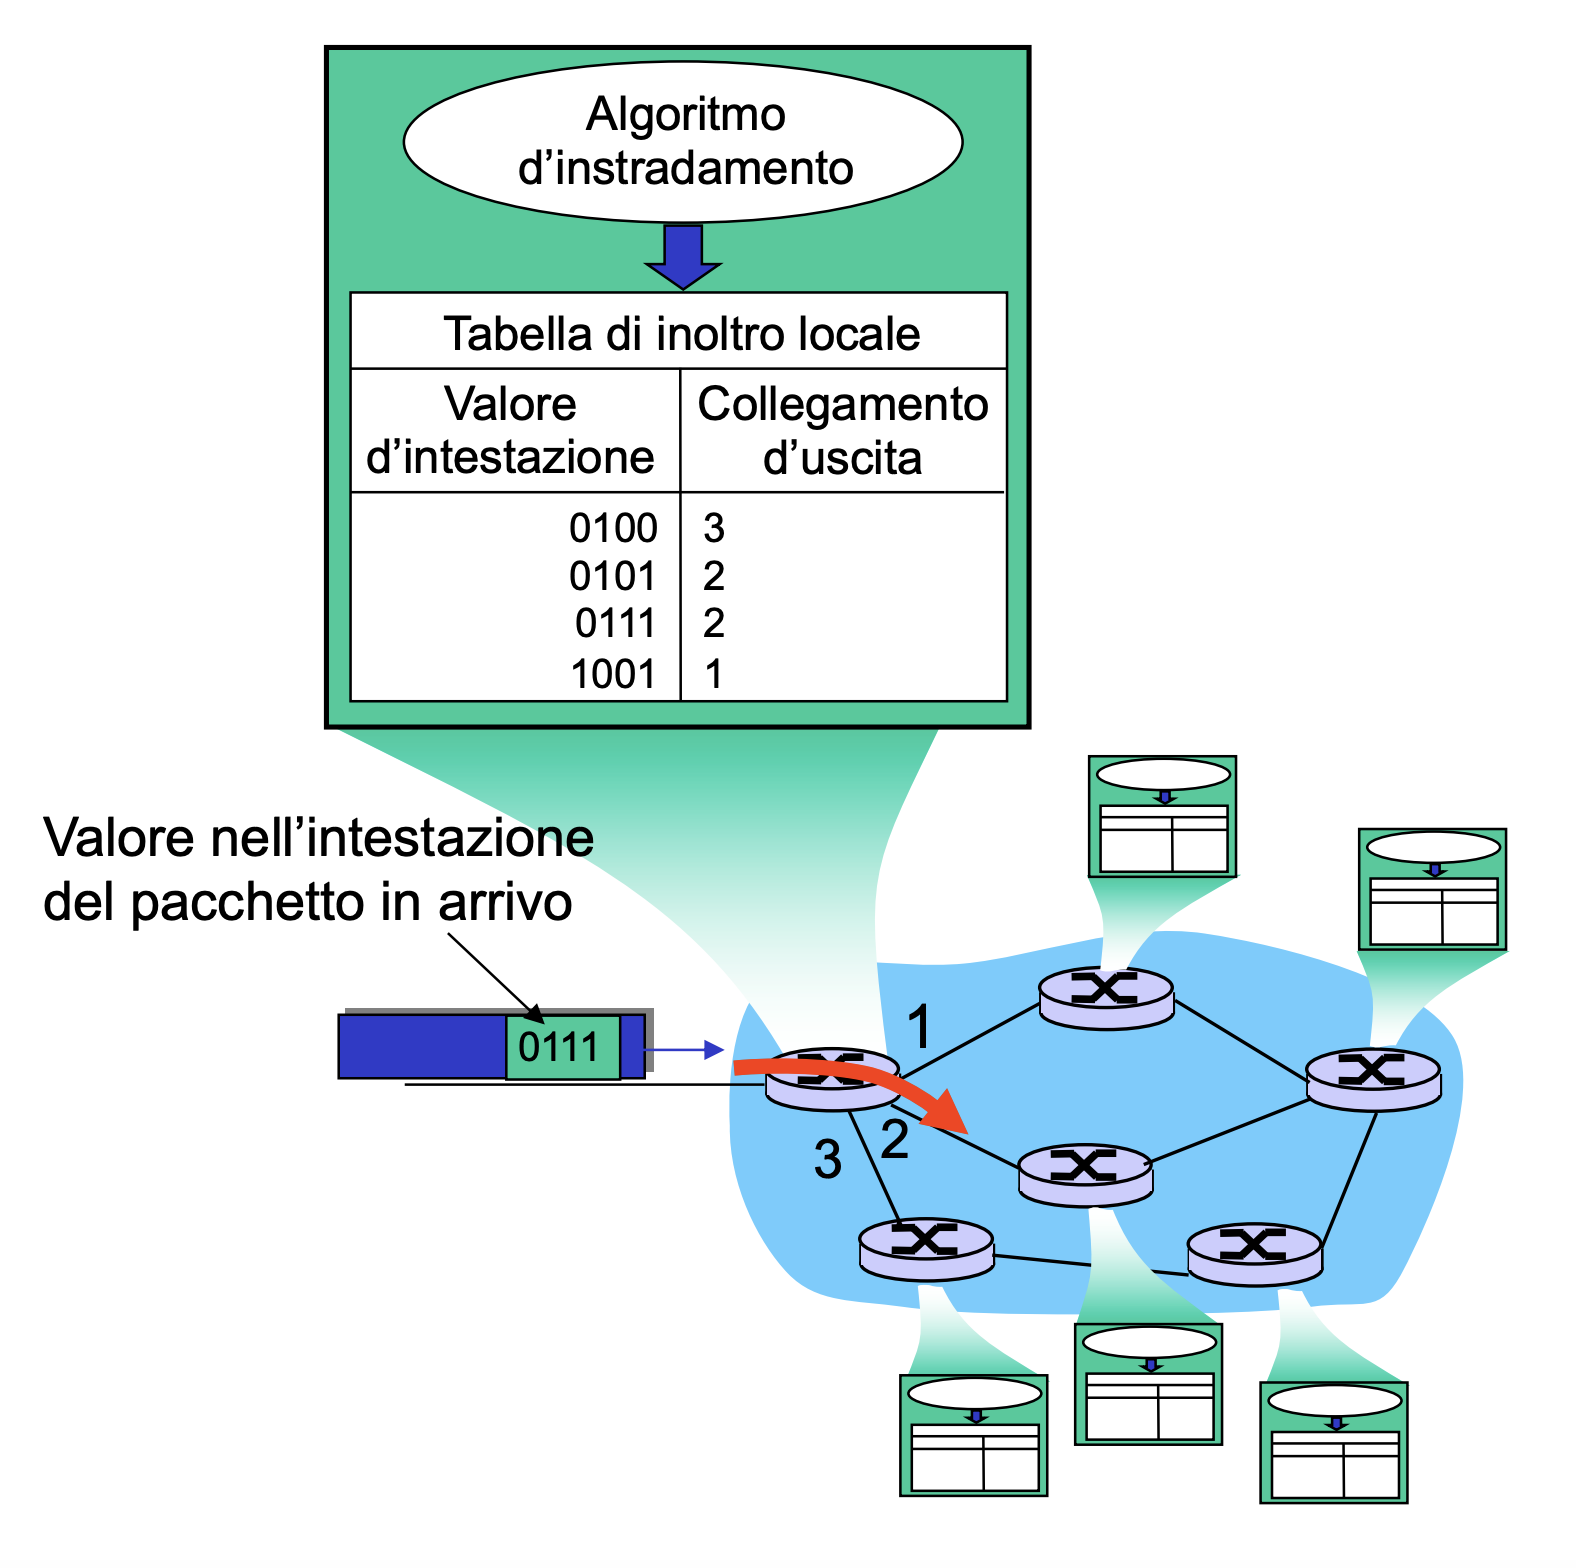
\includegraphics[width=0.5\linewidth]{instradamento}
	\end{center}

Una terza funzione importante del livello di rete è
\textbf{l'impostazione della connessione}, viene utilizzata però solo in
alcune reti (come ATM o X.25). Prima della trasmissione dei dati viene
stabilita una connessione virtuale tra i due host.

\hypertarget{header-n13}{%
\subsection{Modelli di servizio}\label{header-n13}}

Il livello di rete offre diversi modelli di servizio: possiamo ricordare
il servizio \textbf{best effort} utilizzato sulla rete internet attuale
e i modelli \textbf{CBR (Constant), VBR (Variable), ABR (Available),
UBR} utilizzati in ATM, per diversi anni utilizzata alternativa a
Internet.

\hypertarget{header-n15}{%
\section{Reti a circuito virtuale e datagramma}\label{header-n15}}

Le reti a datagramma offrono solo il servizio senza connessione, mentre
le reti a \textbf{circuito virtuale} offrono il servizio con
connessione. Questa è realizzata da host a host e non si può scegliere
(il livello di rete non può fornirli entrambi contemporaneamente).

\hypertarget{header-n17}{%
\subsection{Reti a circuito virtuale}\label{header-n17}}

Le reti a circuito virtuale (come ATM) sono reti analoghe ai circuiti
telefonici che consentono buone prestazioni e vedono il coinvolgimento
della rete: il pacchetto ha un numero di VC nell'header utilizzato e
sostituito dai router, questo numero consente di effettuare
multiplexing.

I router di queste reti mantengono le informazioni sullo stato delle
connessioni, infatti ogni router ha una tabella di inoltro con tutti i
VC utilizzati.

\begin{center}
		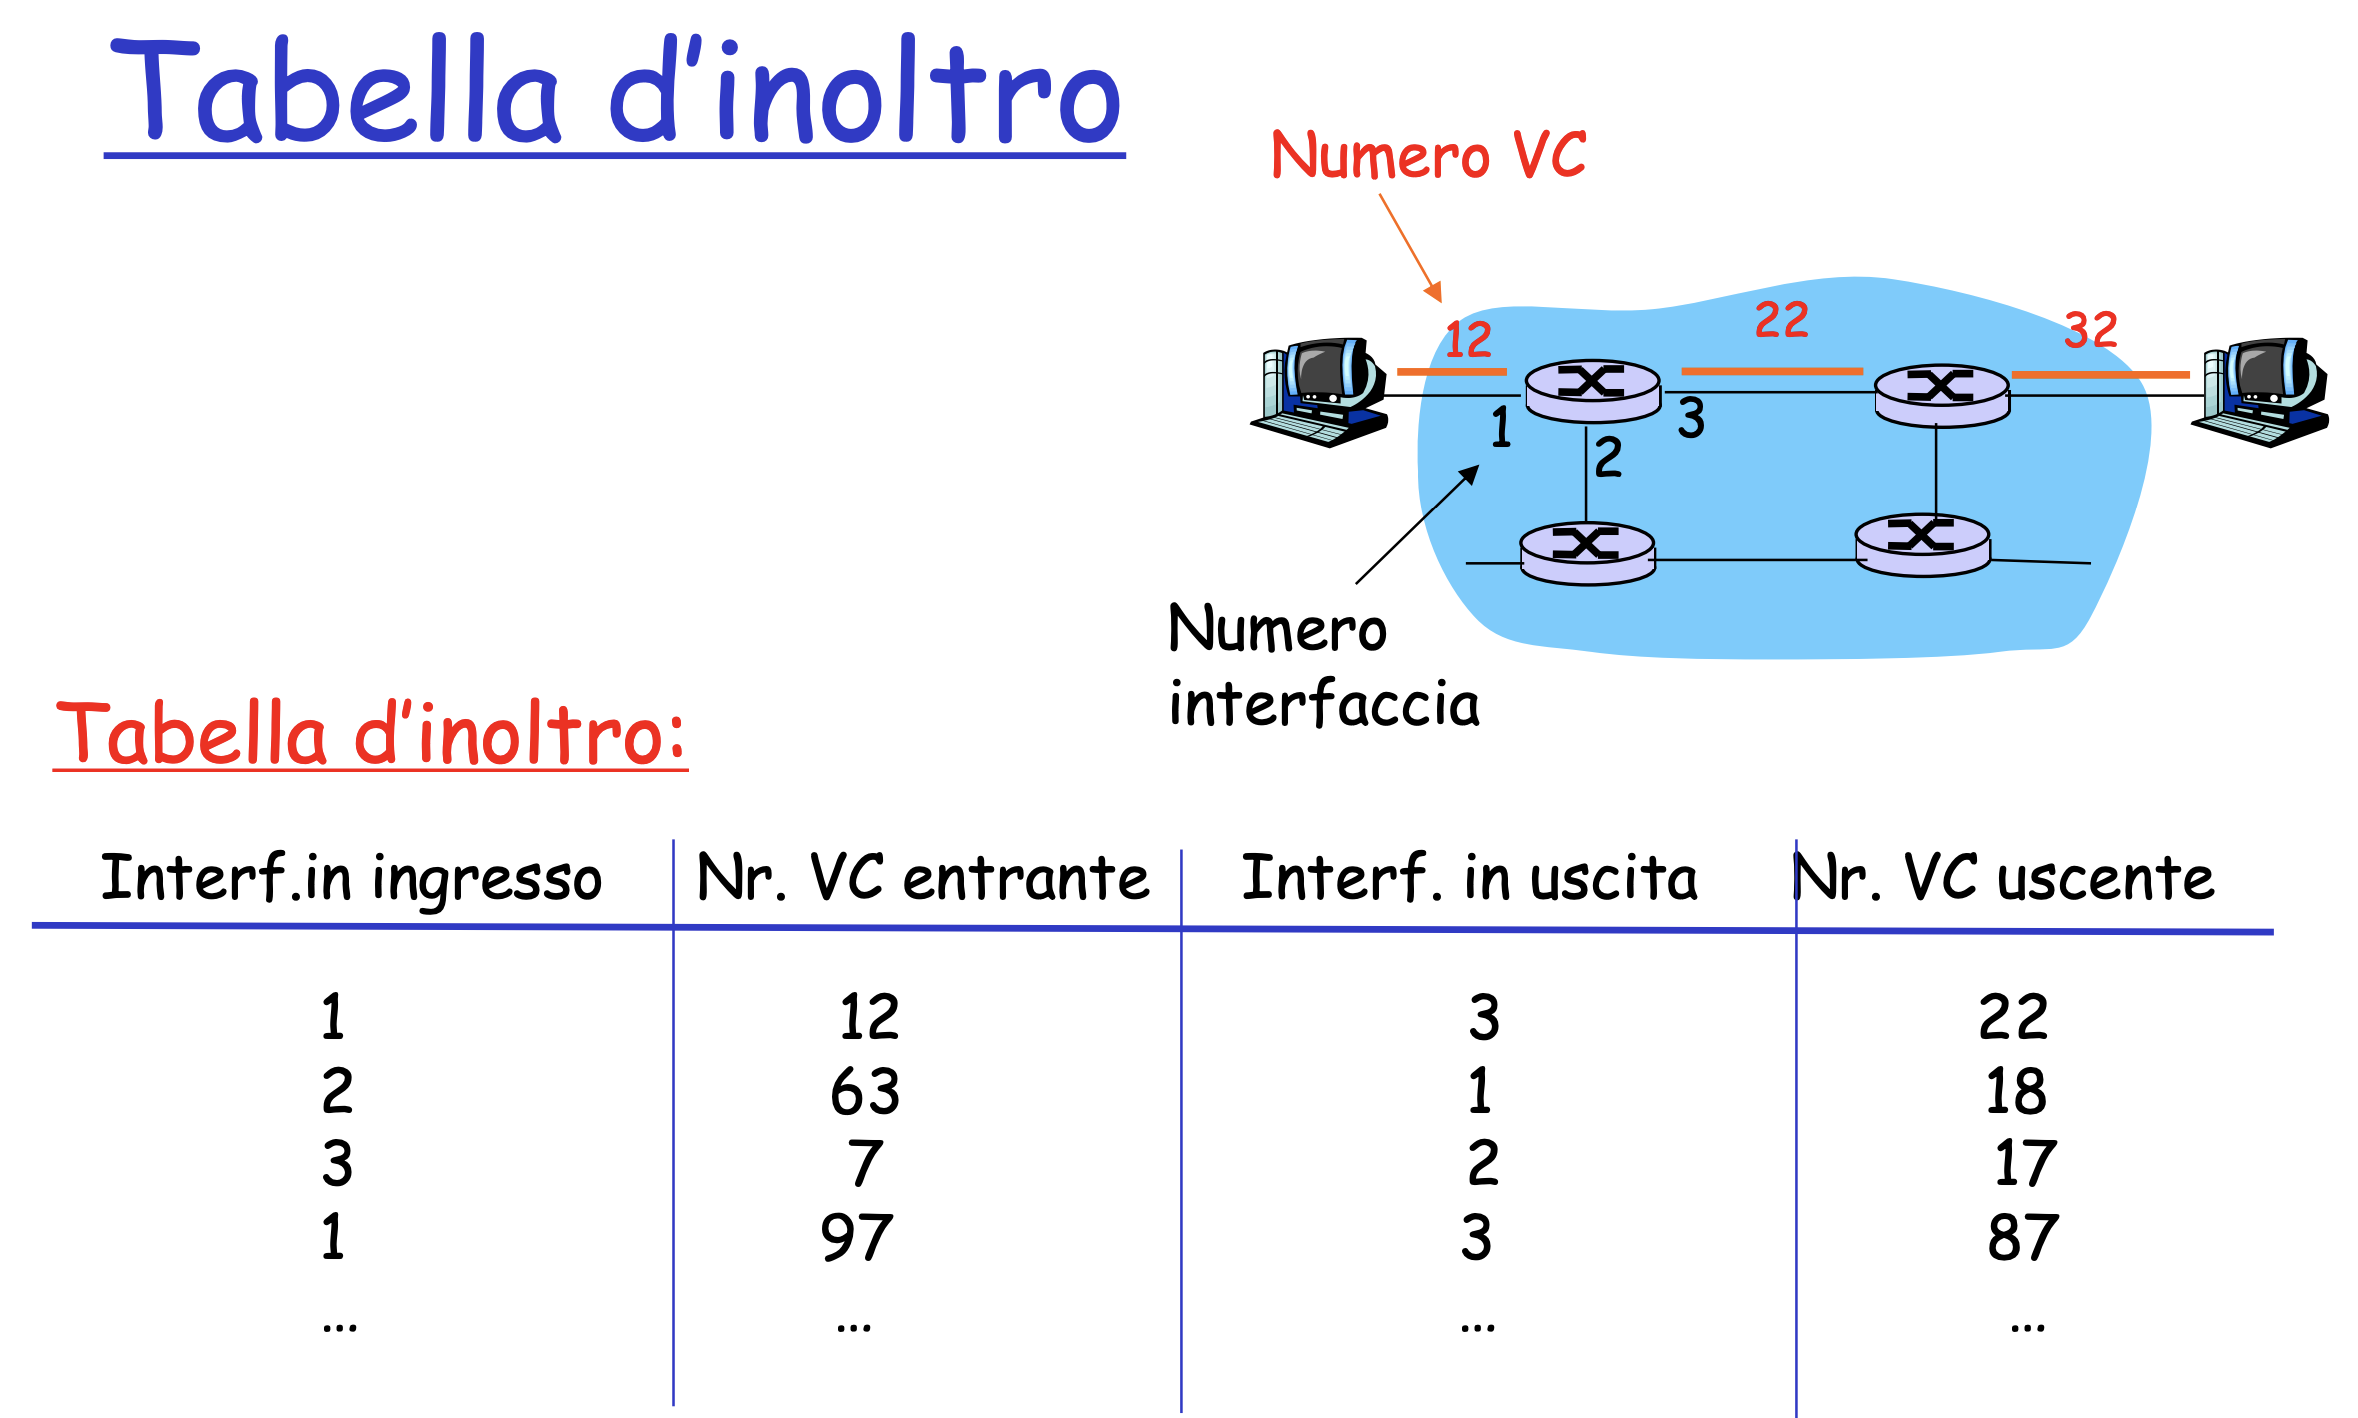
\includegraphics[width=0.7\linewidth]{circuiti-virtuali}
	\end{center}

\hypertarget{header-n21}{%
\subsubsection{Protocolli di segnalazione}\label{header-n21}}

I protocolli di segnalazione, non utilizzati sulla rete Internet, sono
dei messaggi utilizzati per gestire la connessione sui VC quindi avvio,
mantenimento e chiusura dei circuiti.

\hypertarget{header-n23}{%
\subsection{Reti a datagramma}\label{header-n23}}

Nelle reti a datagramma non avviene l'impostazione di chiamata: i dati
vengono inviati quando si vuole e quando la rete può li inoltrerà. In
aggiunta, la rete è stateless (senza connessione) e i pacchetti vengono
inoltrati utilizzando l'indirizzo di destinazione.

Le tabelle di inoltro sono costituite da 4 miliardi di indirizzi
possibili (32 bit), queste tabelle spesso sono realizzate ad intervalli.
Per semplificazione si preferisce effettuare il matching confrontando i
prefissi tra datagram e tabella, nel caso in cui i bit siano uguali si
aumenta il numero di bit confrontati.

\hypertarget{header-n26}{%
\subsection{Confronto tra le due tipologie}\label{header-n26}}

\begin{itemize}
\item
  \textbf{Circuiti virtuali (ATM)}

  \begin{itemize}
  \item
    eredita dalla telefonia
  \item
    requisiti più stringenti in termini di tempo e affidabilità,
    utilizzate per servizi garantiti
  \item
    i terminali sono stupidi: la complessità è interna alla rete (es.
    controllo di flusso)
  \end{itemize}
\item
  \textbf{Datagrammi (internet)}

  \begin{itemize}
  \item
    scambio di dati tra calcolatori
  \item
    i servizi sono elastici: pochi requisiti di tempo
  \item
    L'interconnessione è semplice: adattabile, controllo degli errori,
    rete interna semplice ed ottimizzata alla velocità
  \item
    svariati tipi di link, servizio non uniforme
  \end{itemize}
\end{itemize}

\hypertarget{header-n48}{%
\section{Cosa si trova all'interno dei router?}\label{header-n48}}

\hypertarget{header-n49}{%
\subsection{Architettura}\label{header-n49}}

I router svolgono due funzioni principali:

\begin{itemize}
\item
  far girare i protocolli e gli algoritmi di instradamento (RIP, OSPF,
  BGP)
\item
  inoltrare i datagram dagli input agli output
\end{itemize}

\begin{center}
		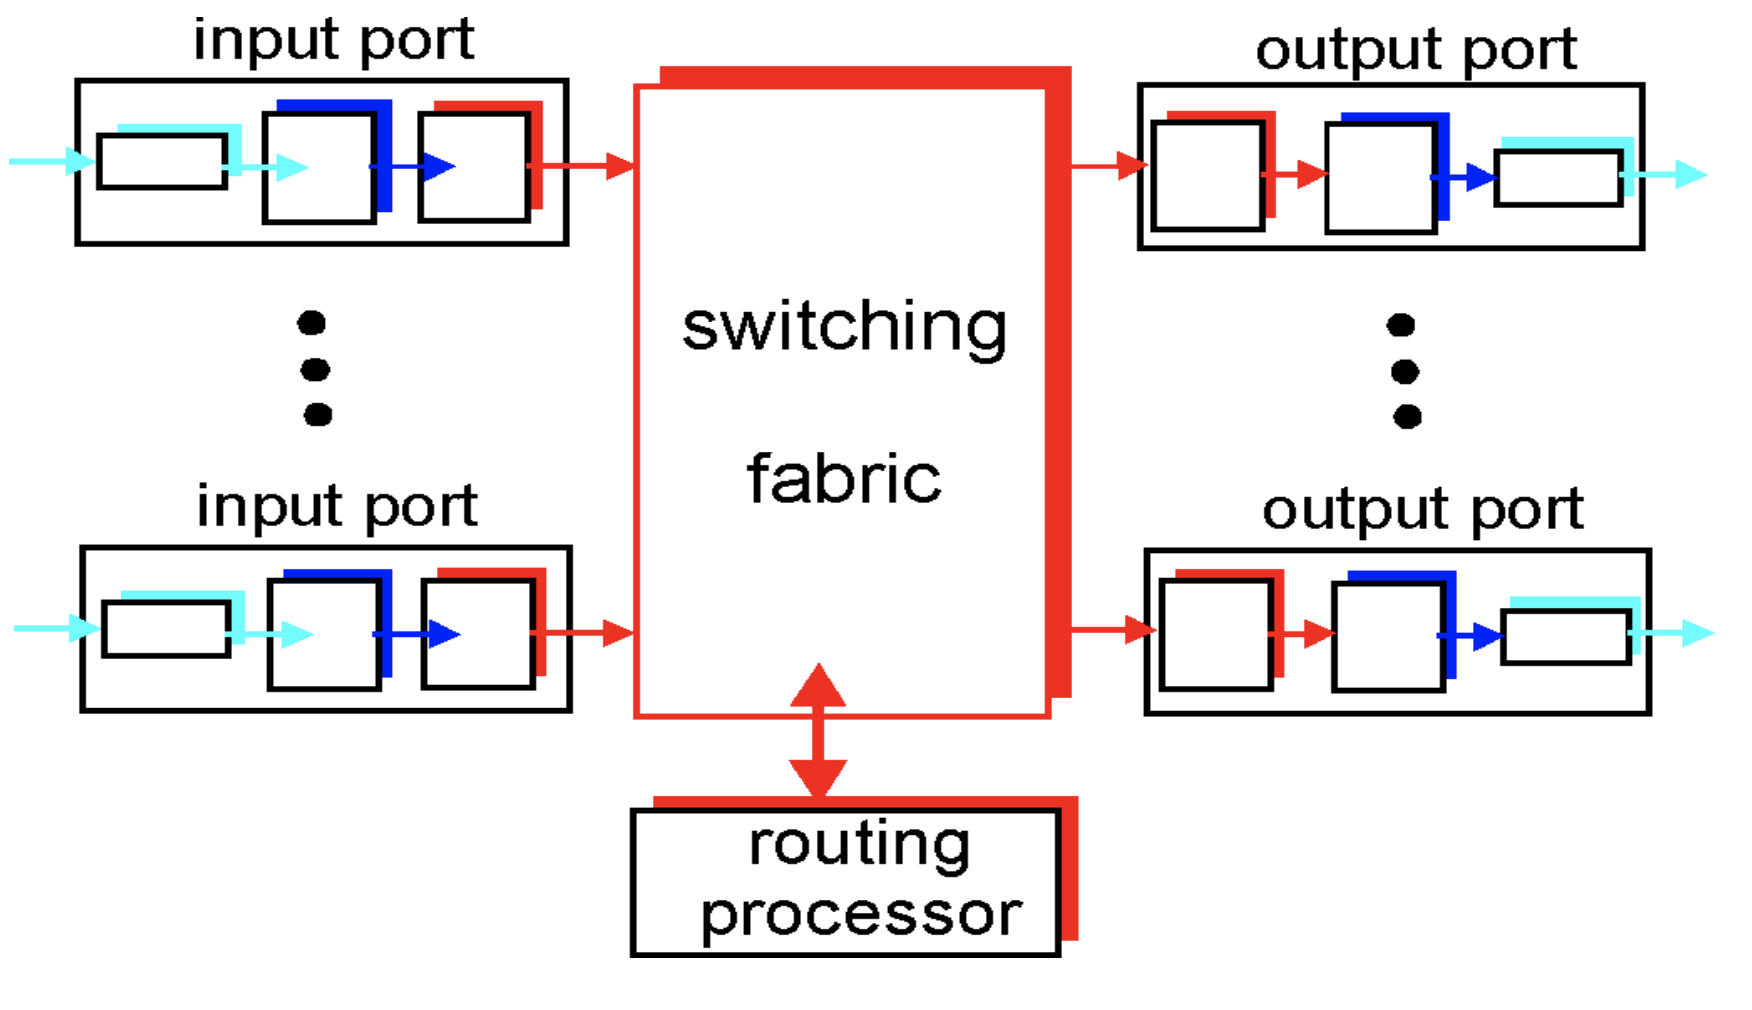
\includegraphics[width=0.7\linewidth]{architettura-router}
	\end{center}

\hypertarget{header-n57}{%
\subsection{Porte d'ingresso}\label{header-n57}}

\begin{center}
		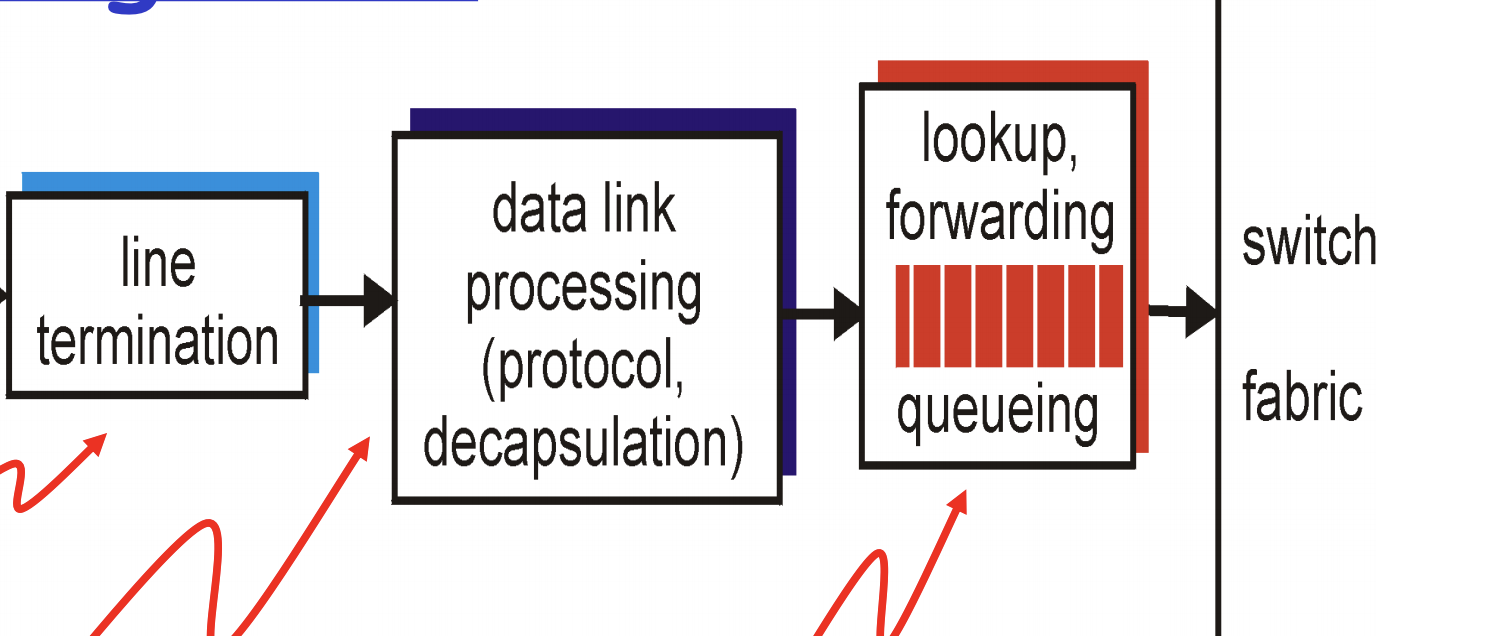
\includegraphics[width=0.7\linewidth]{ingresso-router}
	\end{center}

Le porte d'ingresso dei router vengono utilizzate per effettuare una
commutazione decentralizzata:

\begin{itemize}
\item
  determinare la porta d'uscita dei pacchetti utilizzando le
  informazioni della tabella d'inoltro
\item
  obiettivo: completare l'elaborazione allo stesso tasso della linea
\item
  si presenta un \textbf{accodamento} se il tasso d'arrivo dei pacchetti
  è maggiore del tasso d'inoltro
\end{itemize}

\hypertarget{header-n67}{%
\subsection{Tecniche di commutazione}\label{header-n67}}

\begin{center}
		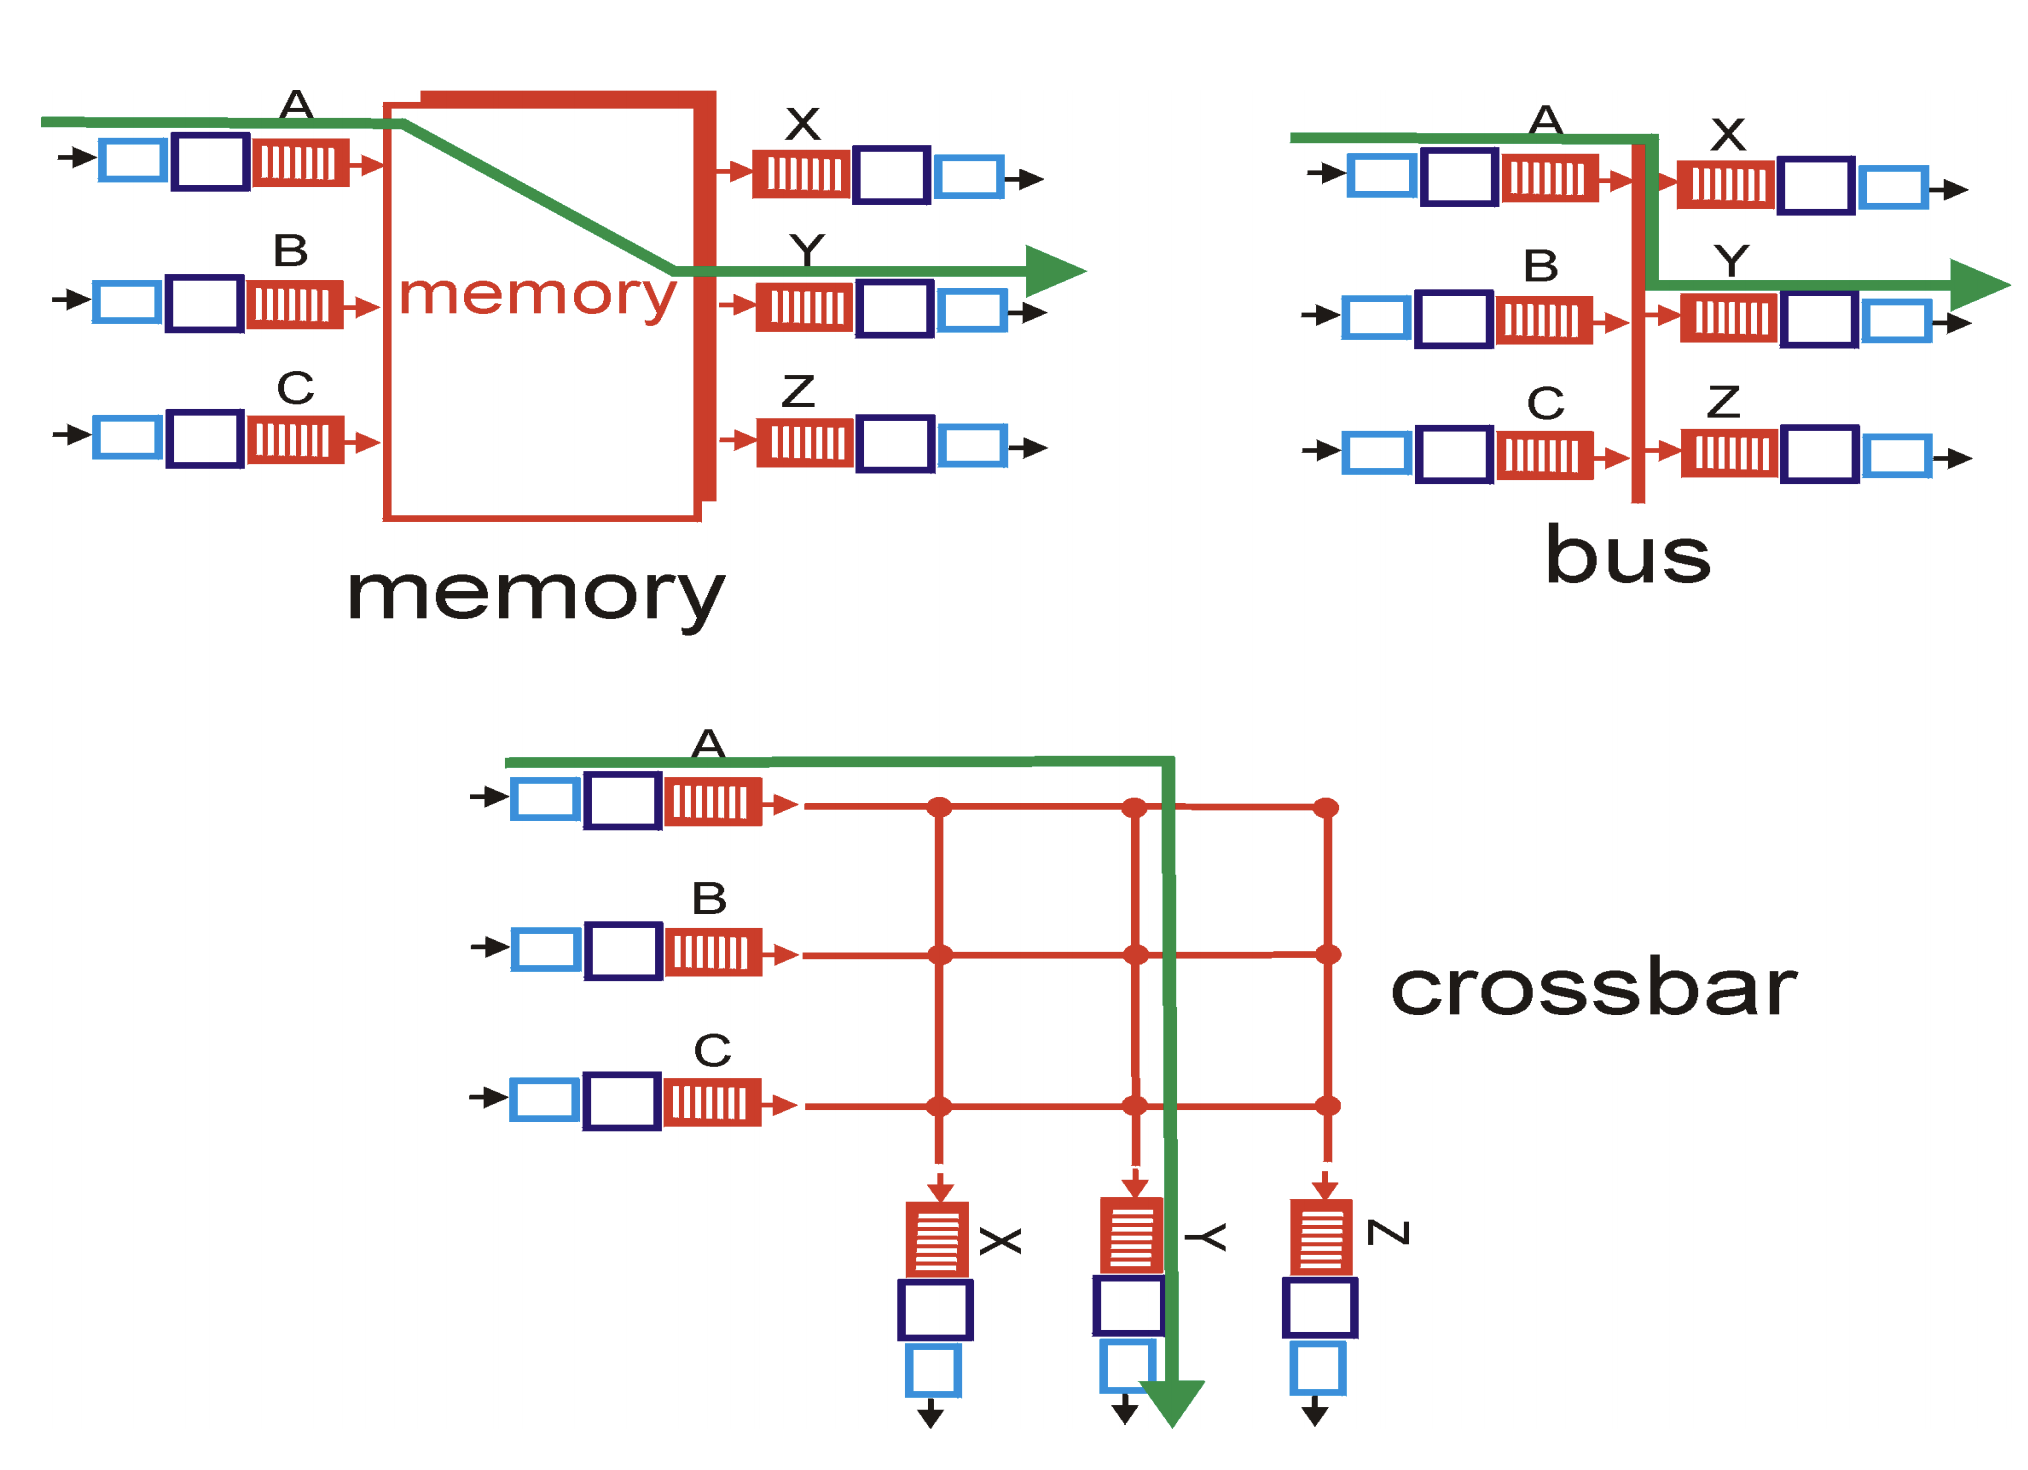
\includegraphics[width=0.7\linewidth]{commutazione}
	\end{center}

La tecnica di commutazione \textbf{in memoria} è la più semplice ma la
meno performante, la tecnica \textbf{a crossbar} è invece la più
efficace.

\hypertarget{header-n70}{%
\subsubsection{Commutazione in memoria}\label{header-n70}}

La tecnica di commutazione in memoria veniva utilizzata nelle prime
generazioni di router, i quali erano tradizionali calcolatori. La
commutazione veniva controllata dalla CPU: il pacchetto veniva copiato
in memoria e successivamente mandato in uscita con una frequenza totale
di \textbf{B/2}.

\hypertarget{header-n72}{%
\subsubsection{Commutazione tramite bus}\label{header-n72}}

La commutazione tramite bus si basa sull'utilizzo di un bus condiviso
tra tutte le porte: siamo in presenza di una \textbf{contesa per il
bus}, la cui banda limita di conseguenza la banda della commutazione.

Un esempio di router è il Cisco 5600, che opera con un bus da 32 Gbps,
sufficiente per reti d'accesso o aziendali.

\hypertarget{header-n75}{%
\subsubsection{Commutazione attraverso rete
d'interconnessione}\label{header-n75}}

Questa tecnica supera il limite di banda di un bus condiviso. Viene
utilizzato un \textbf{crossbar switch}, ovvero una rete
d'interconnessione di \emph{2n} bus che collegano \emph{n} porte
d'entrata a \emph{n} porte d'uscita.

Un esempio come il Cisco 12000 raggiunge i 60 Gbps nella struttura di
commutazione.

\hypertarget{header-n78}{%
\subsection{Porte d'uscita}\label{header-n78}}

Le porte d'uscita implementano le funzioni di accodamento (se la
frequenza di pacchetti in arrivo è superiore a quella del collegamento
uscente) e di schedulatore di pacchetti (stabilire l'ordine di
trasmissione dei pacchetti).

\hypertarget{header-n80}{%
\subsection{Quale deve essere la capacità dei
buffer?}\label{header-n80}}

Secondo la regola spannometrica della RFC 3439 la capacità deve essere

\[media \space RTT \space*\space capacita \space C\]

dove C è la capacità del collegamento.

Secondo attuali raccomandazioni, dati N flussi la capacità dei buffer
deve essere

\[\frac{RTT*C}{\sqrt{N}}\]

\hypertarget{header-n86}{%
\section{Protocollo Internet (IP)}\label{header-n86}}

\begin{center}
		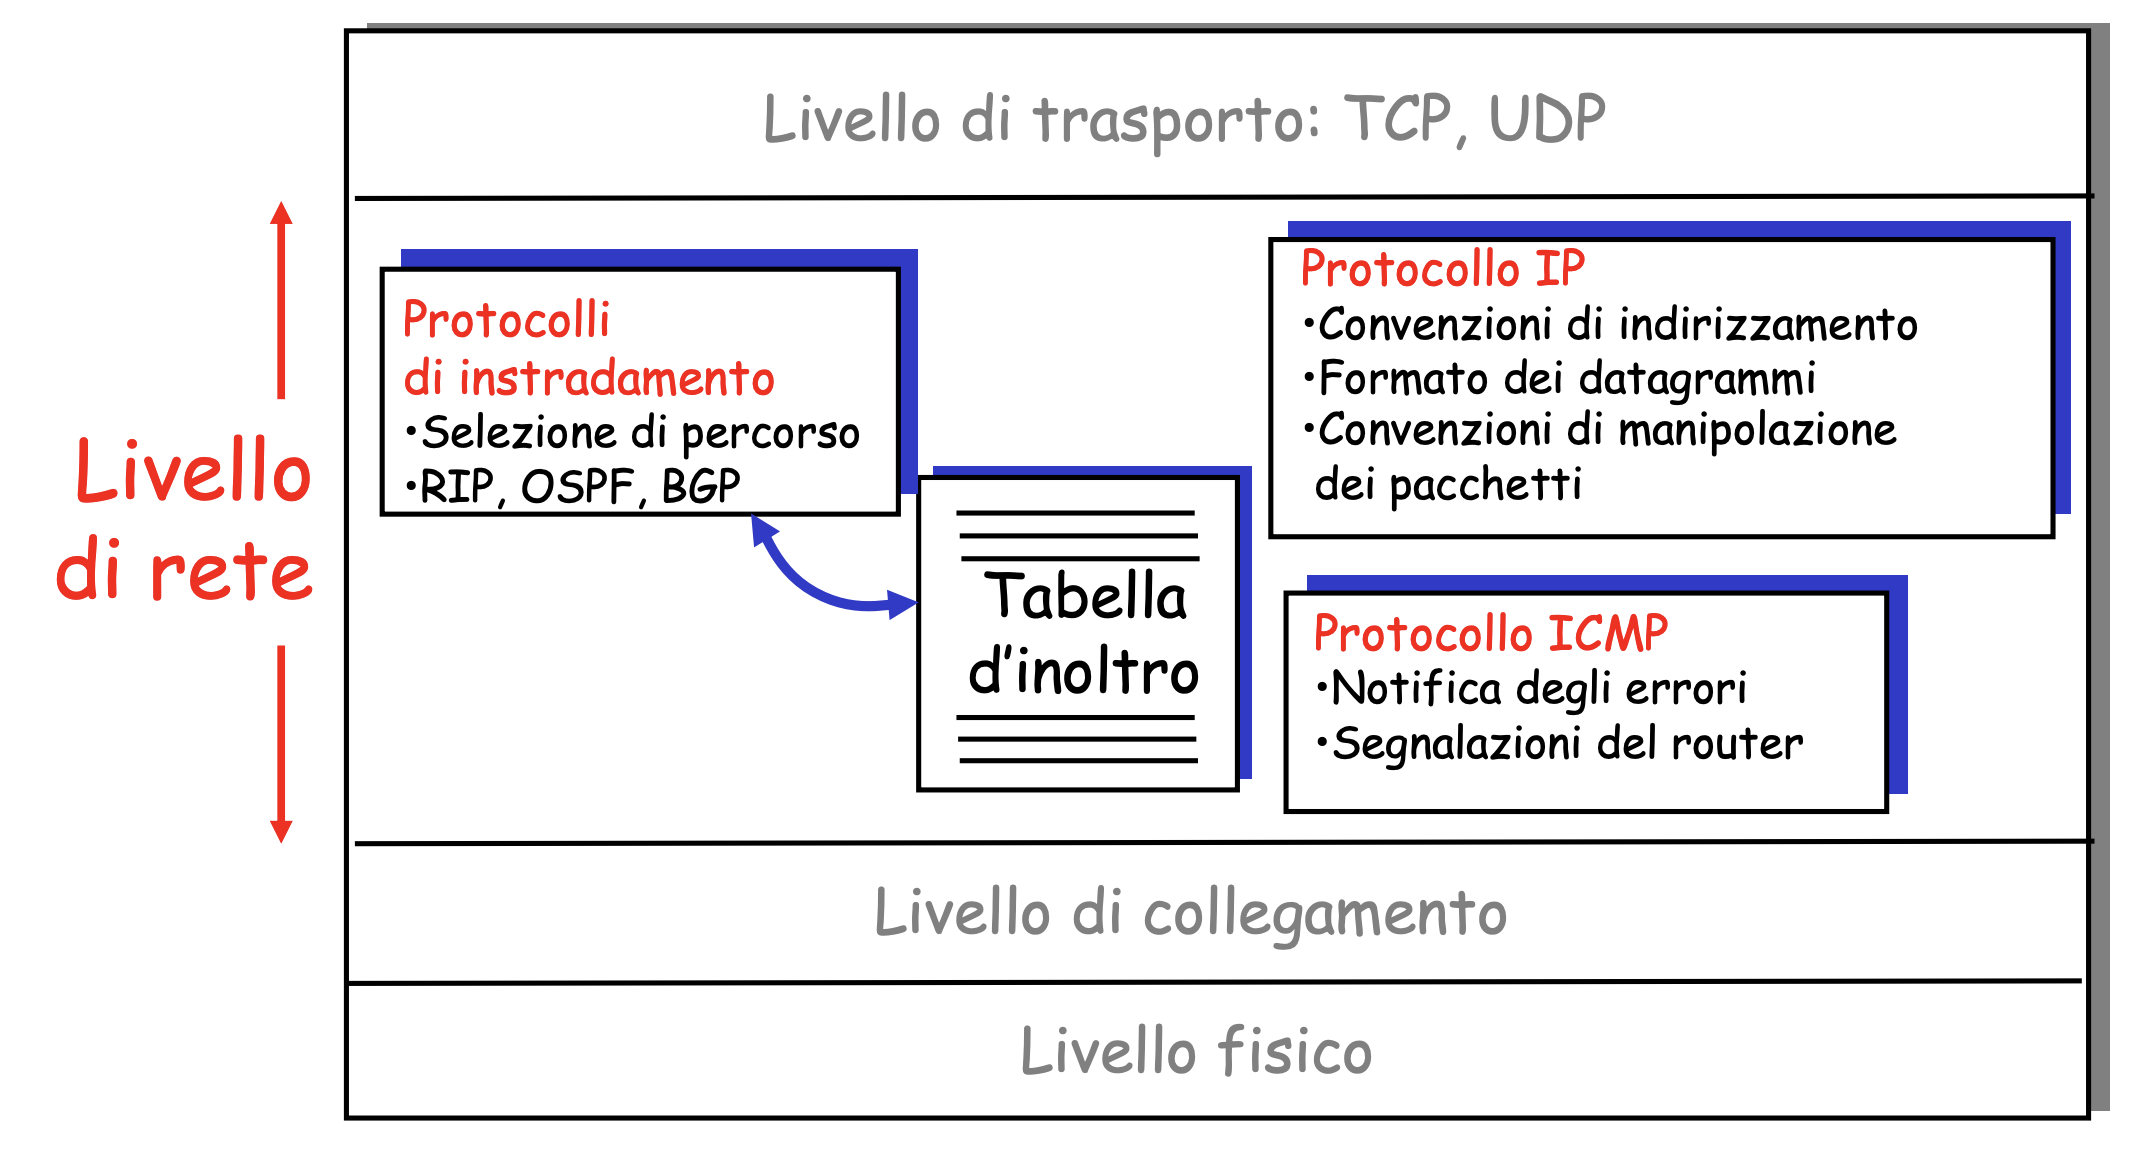
\includegraphics[width=0.7\linewidth]{liv-rete}
	\end{center}

\hypertarget{header-n88}{%
\subsection{Formato dei datagrammi}\label{header-n88}}

\begin{center}
		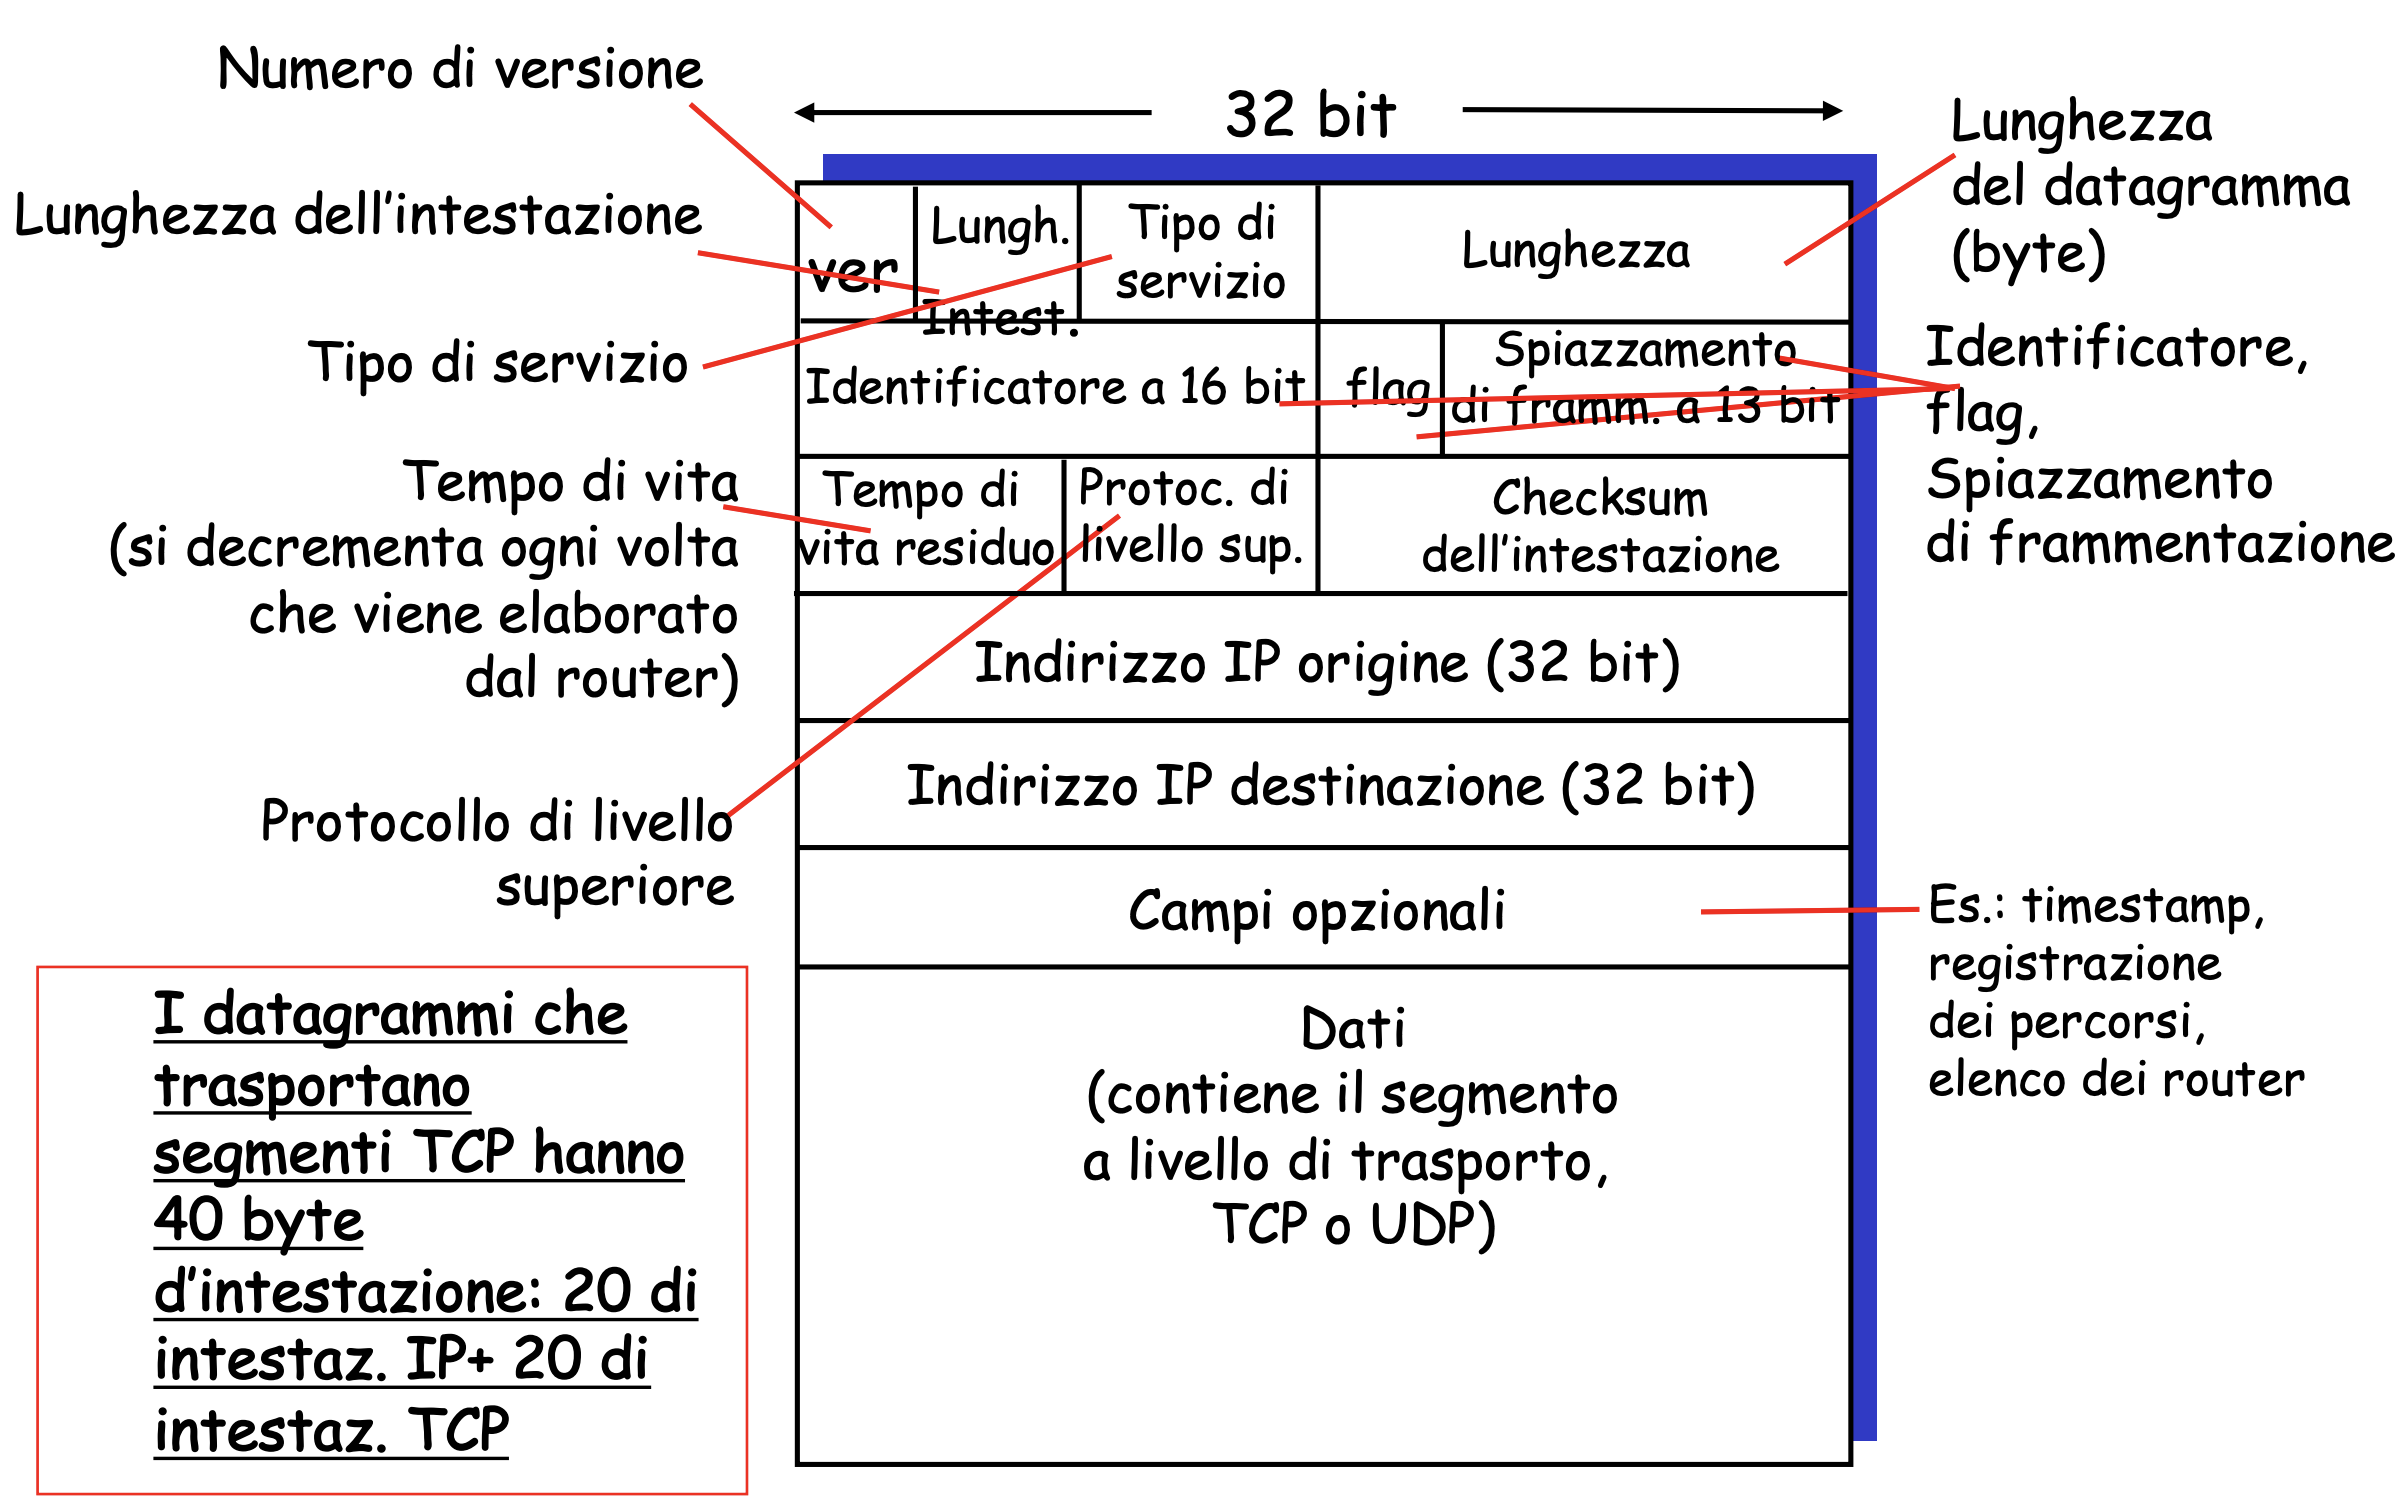
\includegraphics[width=0.7\linewidth]{datagram-ip}
	\end{center}

Il campo lunghezza del datagramma è da 16 bit, i datagram  hanno quindi una dimensione massima
di 64 KB. Il campo del protocollo di livello superiore indica il
protocollo utilizzato dal pacchetto trasmesso, quindi TCP/UDP. Avendo a
disposizione 32 bit per gli indirizzi abbiamo in totale poco più di 4
miliardi di indirizzi.

\hypertarget{header-n91}{%
\subsubsection{Frammentazione dei datagrammi}\label{header-n91}}

La frammentazione dei datagrammi è una funzione importante poiché
consente il trasporto da parte del livello sottostante (collegamento) di
datagrammi più grandi di quanto ne potrebbe portare.

Se la \textbf{MTU} (Maximum Transmission Unit, quantità massima di dati
che un frame a livello di collegamento può portare) è più bassa della
dimensione del datagram IP, il livello 3 frammenta i datagram troppo
grossi in altri datagram, che verranno riassemblati solo a destinazione.
Ogni router della rete può frammentare in base alle sue esigenze.

Quando viene effettuata la frammentazione viene settato a 1 il flag
relativo nell'header di ogni pacchetto inviato (tranne l'ultimo) e in
ognuno viene indicato lo spiazzamento (utilizzato per riposizionare il
datagramma nel giusto payload e in posizione corretta).

Lo spiazzamento viene calcolato come numero di byte dati presenti nei datagram precedenti (senza contare i 20 byte di header) / 8.

\begin{wrapfigure}{r}{0.4\textwidth}
		\centering
		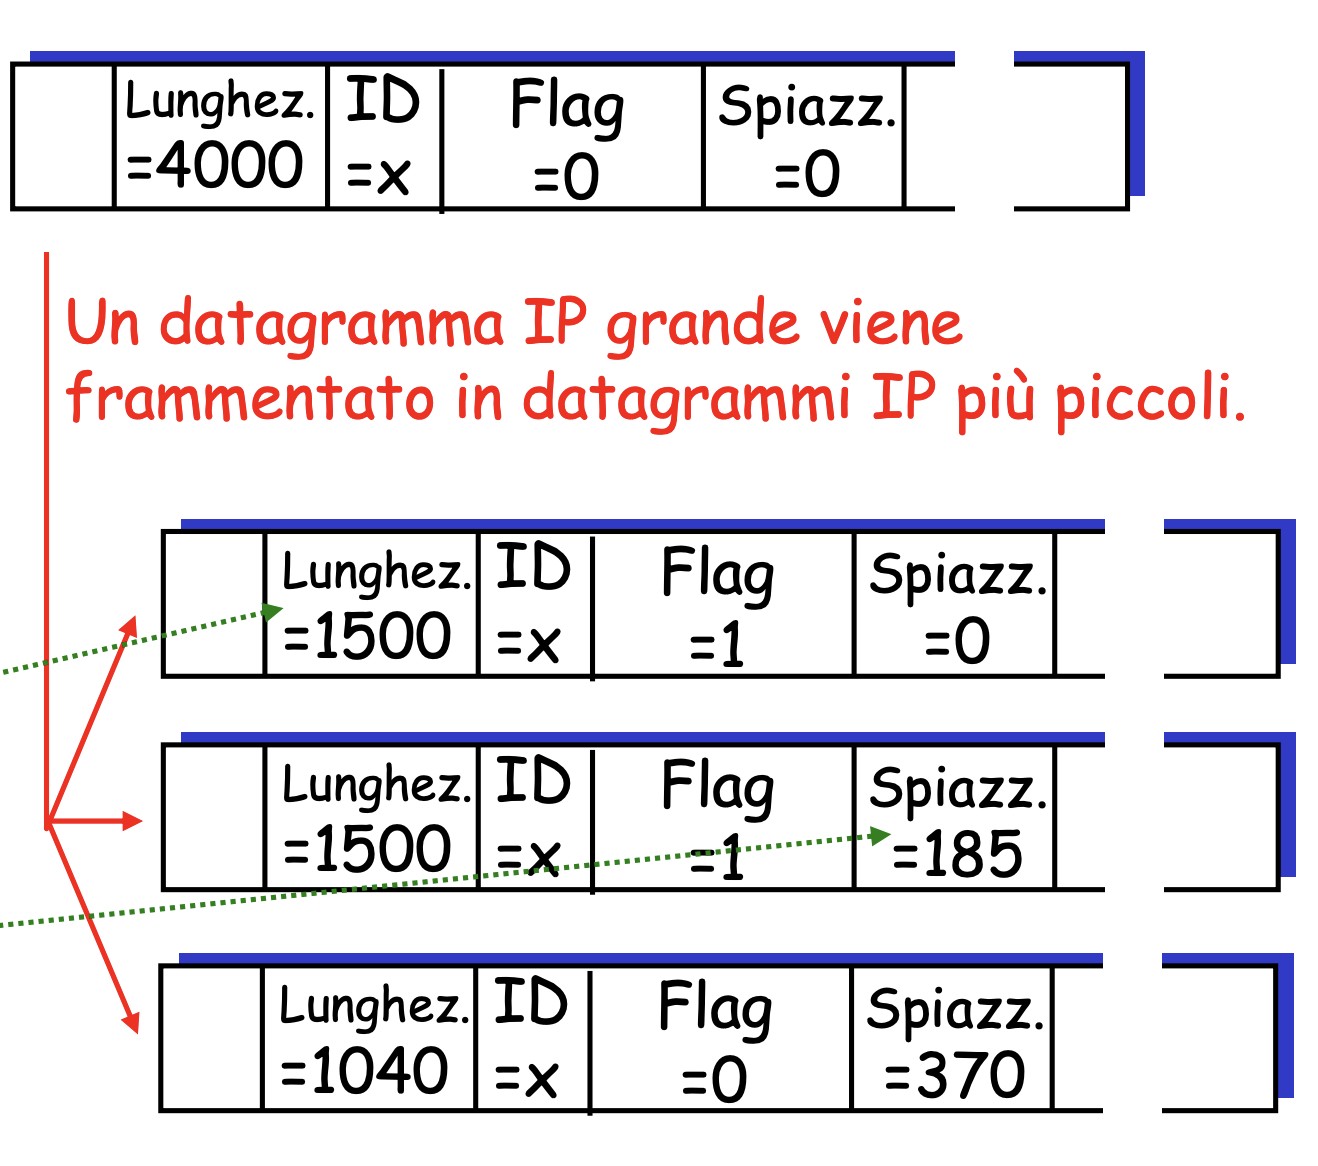
\includegraphics[width=0.4\textwidth]{frammentazione}
		\vspace{-30pt}
	\end{wrapfigure}

Il destinatario ricostruirà il datagram originale riconoscendo gli ID
comuni, sapendo che se lo spiazzamento è uguale a 0 sarà il primo,
mentre se il flag sarà uguale a 0 sarà l'ultimo.

\hypertarget{header-n97}{%
\subsection{Indirizzamento IPv4}\label{header-n97}}

L'indirizzamento IPv4 consente il posizionamento dei dispositivi nella
rete globale: infatti, ogni \textbf{interfaccia} di ciascun host
collegato su Internet ha un IP globalmente univoco. Questo indirizzo è
costituito da 32 bit.

L'interfaccia è il confine tra host e collegamento fisico: i router
devono avere almeno due interfacce (2 indirizzi IP) mentre gli host, in
genere, hanno una sola interfaccia.

\hypertarget{header-n100}{%
\subsubsection{Sottoreti}\label{header-n100}}

Le sottoreti consentono di dividere l'indirizzamento in Internet in
parti a sè stanti. Per dare una definizione appropriata possiamo
considerare le sottoreti come delle reti isolate i cui punti terminali
sono collegati all'interfaccia di un host o un router.

Questo è possibile suddividendo gli indirizzi IP in due parti: una parte
di \textbf{sottorete}, condivisa fino a un certo punto, e una parte di
\textbf{host}.

\begin{center}
		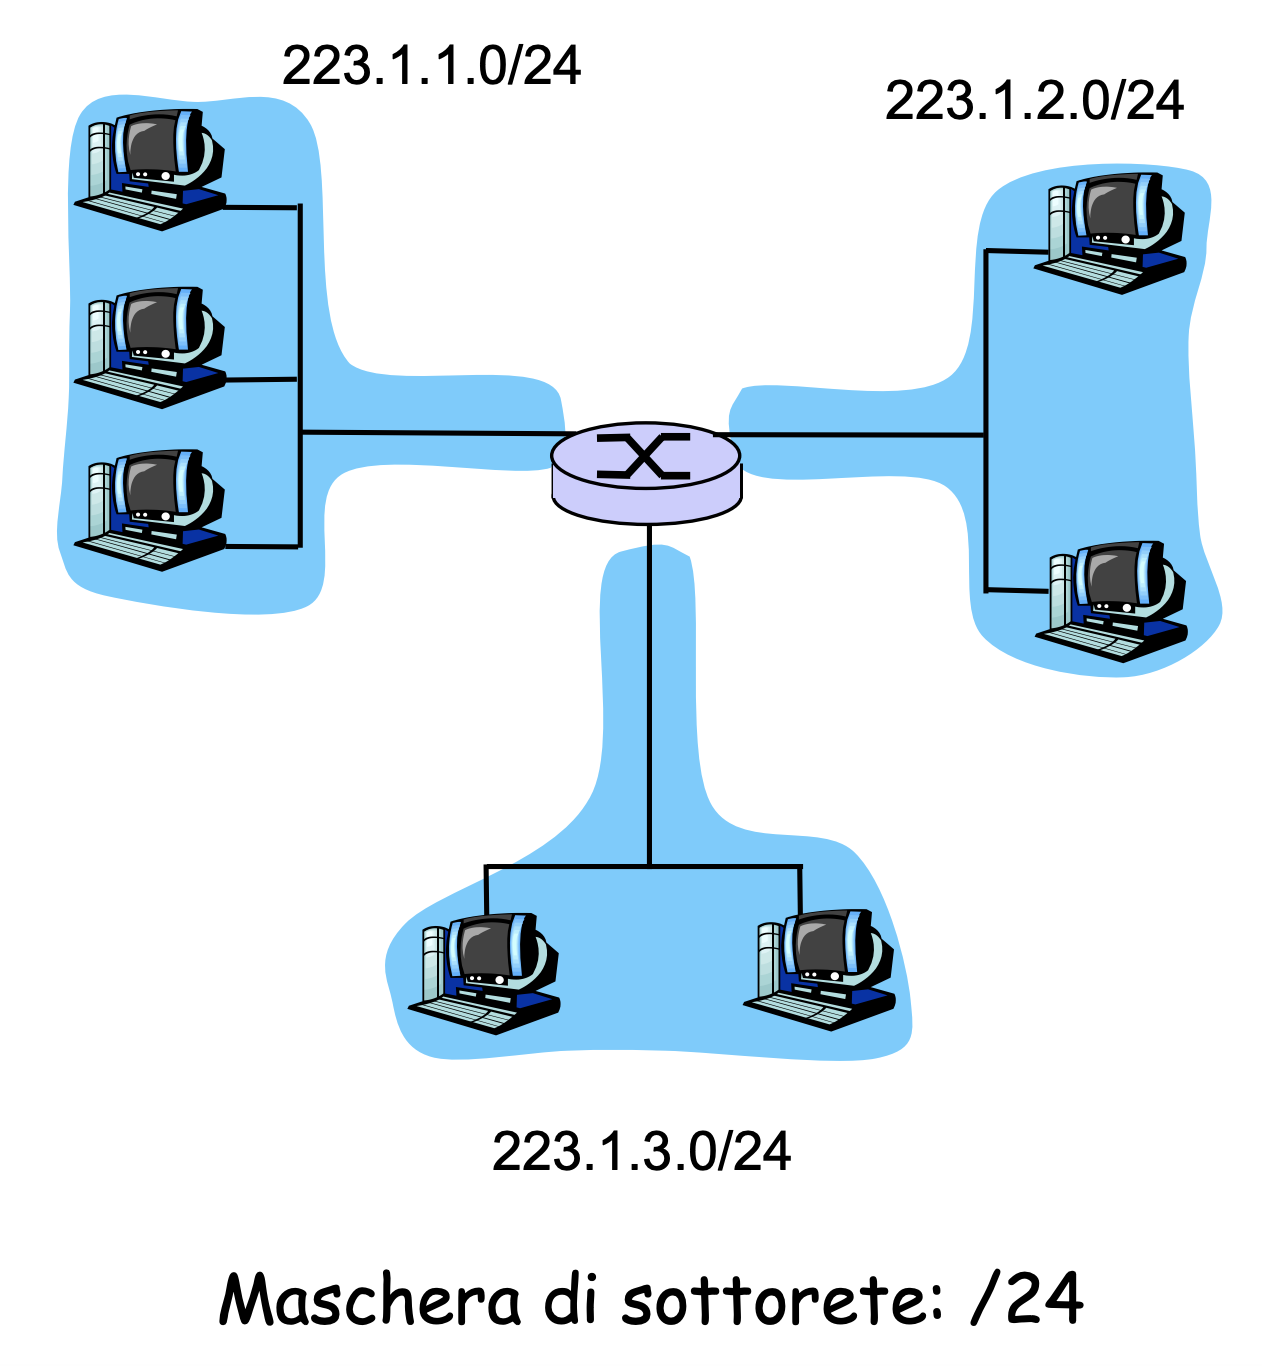
\includegraphics[width=0.7\linewidth]{subnet}
	\end{center}

La \textbf{maschera di rete} viene utilizzata per indicare quanti bit da
sinistra contengono il prefisso condiviso tra tutti gli host della
sottorete.

\hypertarget{header-n105}{%
\paragraph{CIDR}\label{header-n105}}

CIDR, o (Classless Interdomain Routing), è una strategia di assegnazione
degli indirizzi che definisce il prefisso comune agli apparati in una
rete.

Ha una struttura del tipo \emph{a.b.c.d/x} dove x indica il numero di
bit della prima parte dell'indirizzo (parte subnet).

\begin{center}
		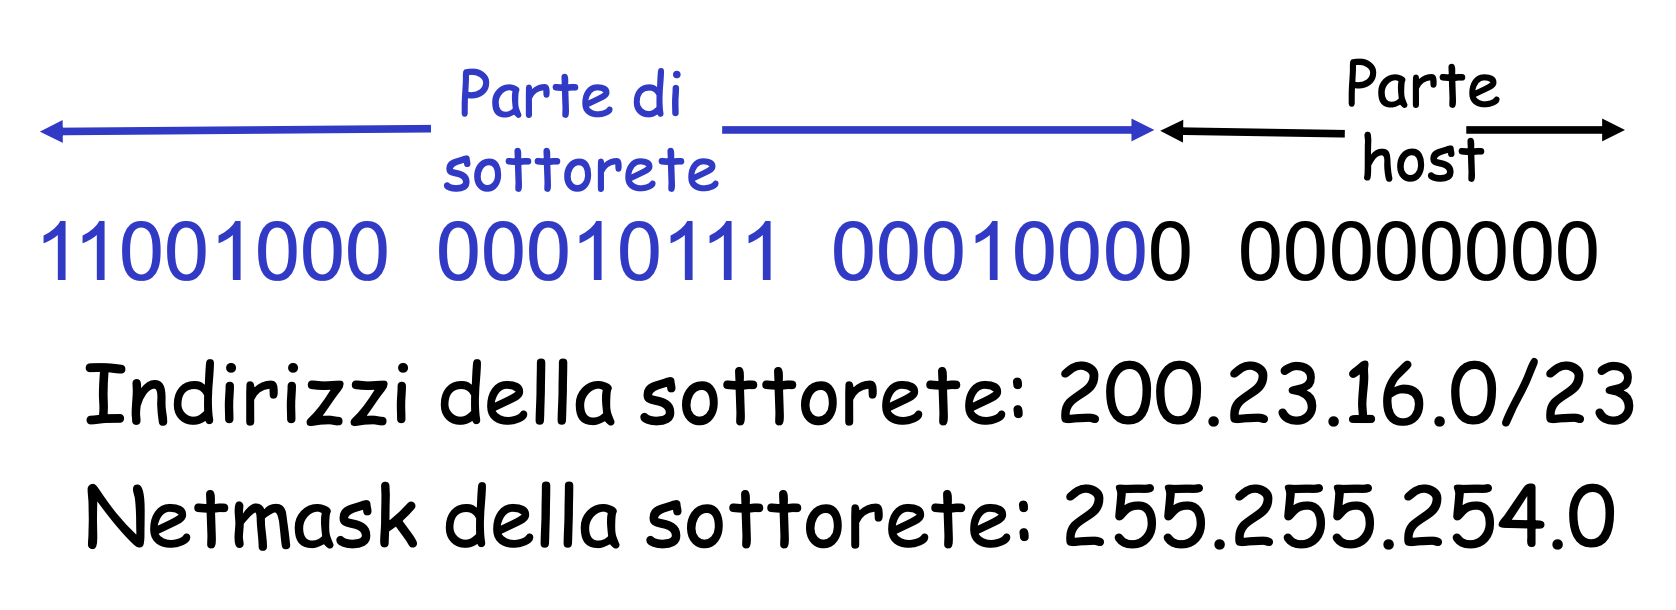
\includegraphics[width=0.5\linewidth]{cidr}
	\end{center}

La strategia CIDR facilita ai router la costruzione delle tabelle di
inoltro e consente a un PC di sapere se un host si trova nella sua
stessa sottorete (facendo l'AND tra indirizzo e maschera di rete troverà
il prefisso che confronterà).

\hypertarget{header-n110}{%
\subsubsection{Assegnazione degli indirizzi}\label{header-n110}}

L'assegnazione degli indirizzi può avvenire in modalità manuale o
mediante \textbf{DHCP}. Il DHCP (Dynamic Host Configuration Protocol)
consente di ottenere dinamicamente un IP da un server (plug-and-play),
l'IP avrà una scadenza e potrà essere rinnovato, consente il riuso e il
risparmio di indirizzi.

\begin{center}
		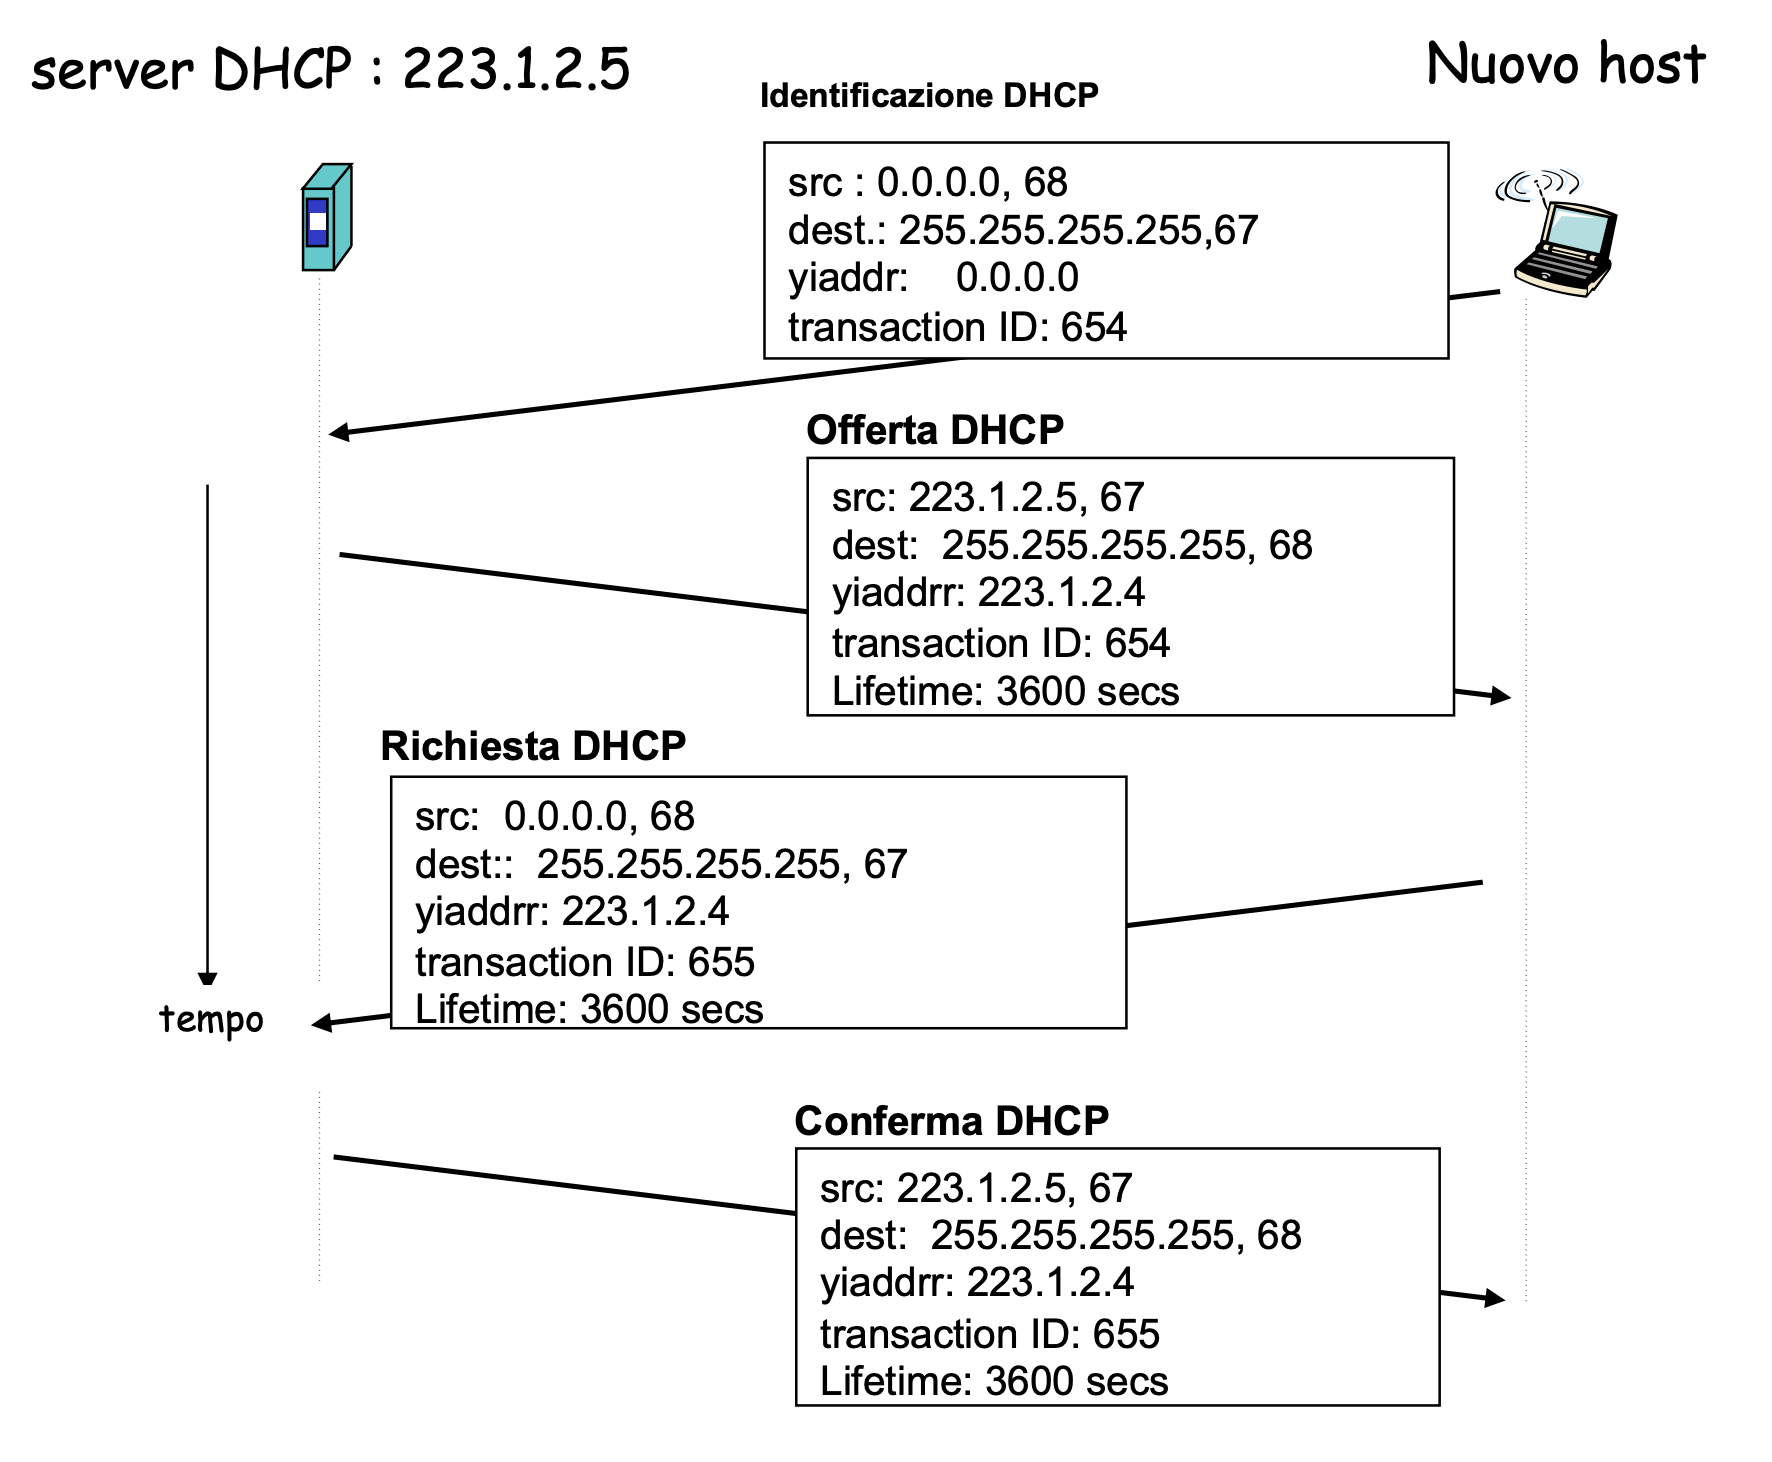
\includegraphics[width=0.7\linewidth]{dhcp}
	\end{center}

L'amministratore di rete o l'ISP ha a disposizione un blocco di IP da
utilizzare nelle subnet: se sono privati non si pone alcun problema,
mentre se sono pubblici questi dovranno essere comprati da altri ISP. A
sua volta, un ISP o un amministratore può dividere il blocco a sua
disposizione in altri sottoblocchi contigui.

\hypertarget{header-n115}{%
\paragraph{Indirizzamento gerarchico}\label{header-n115}}

\begin{center}
		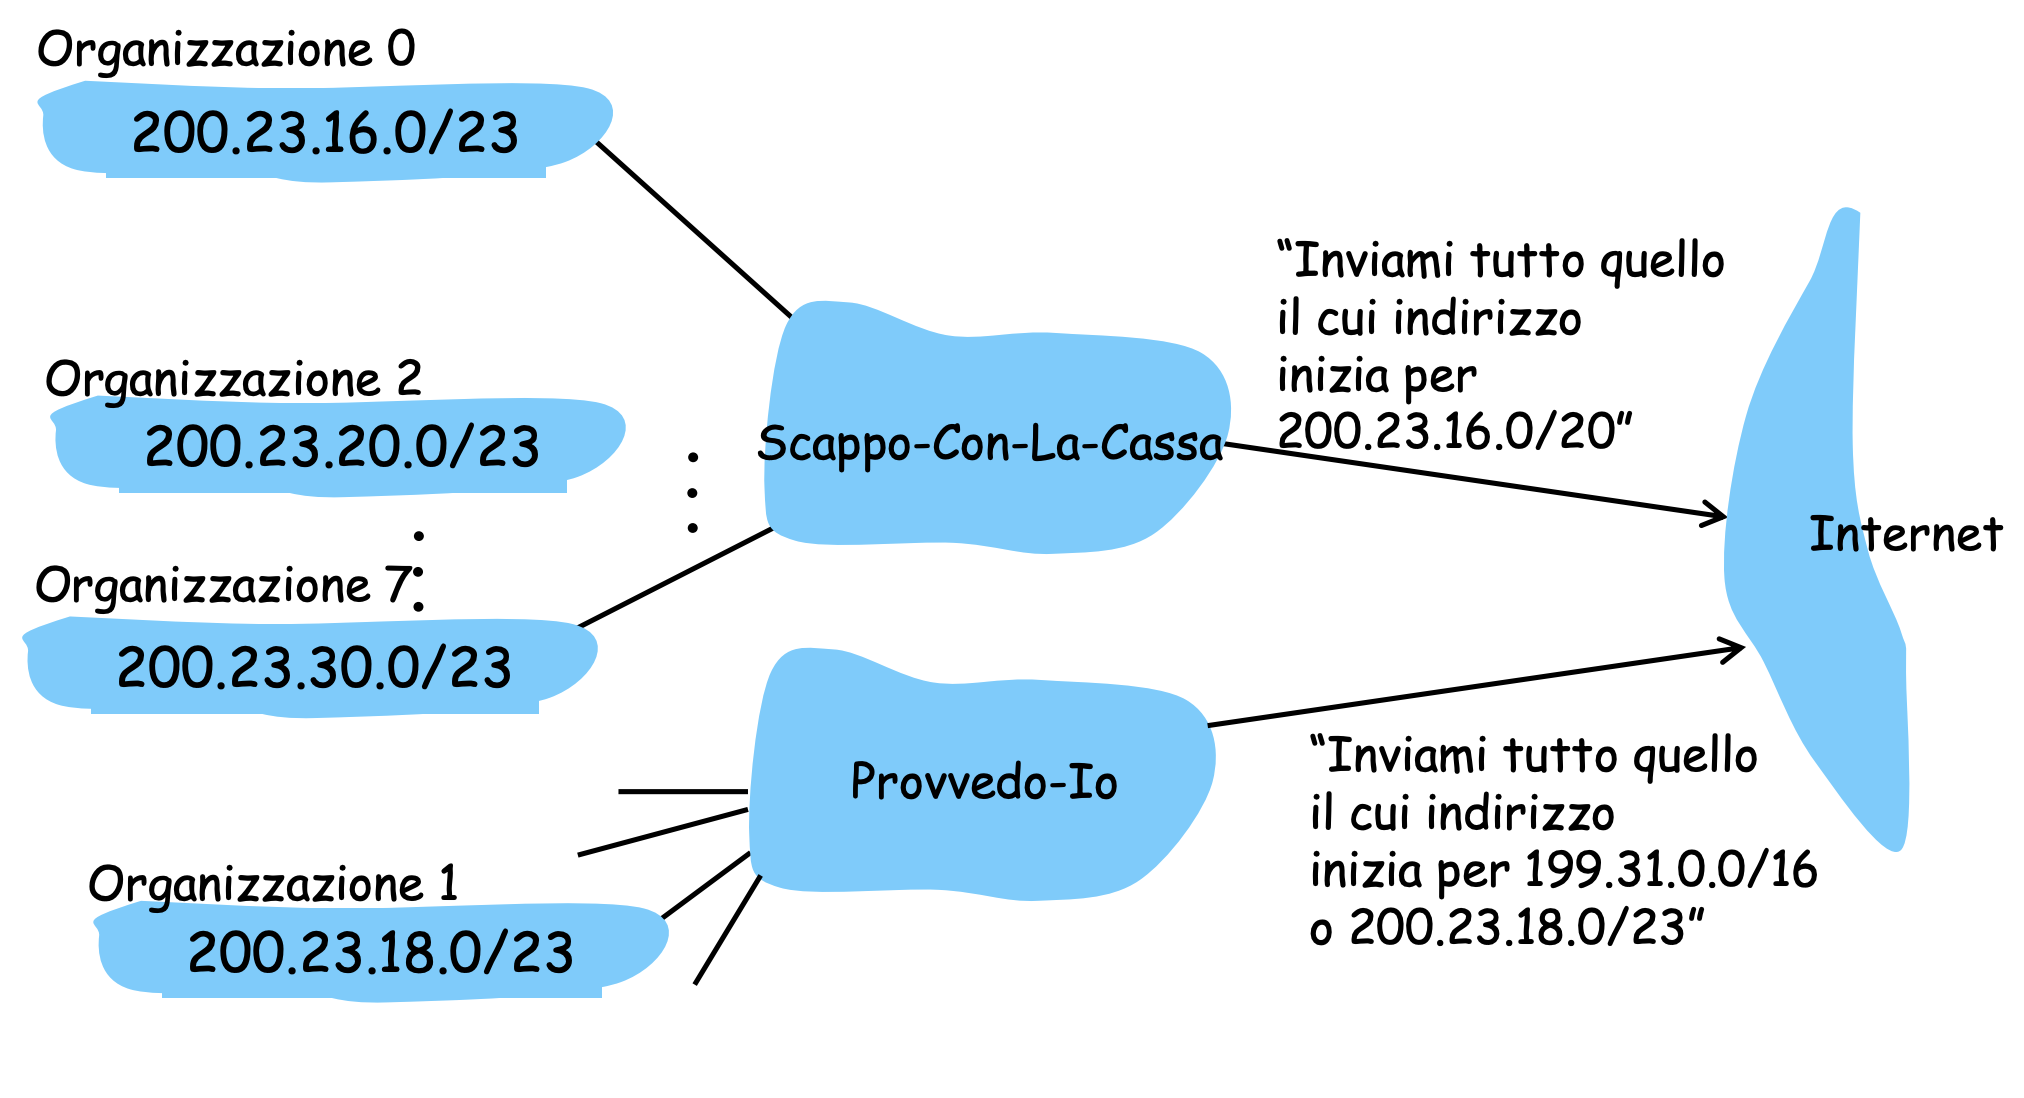
\includegraphics[width=0.7\linewidth]{ind-gerarchico}
	\end{center}

\hypertarget{header-n117}{%
\paragraph{Indirizzi IP alla fonte}\label{header-n117}}

Come fa un ISP a ottenere indirizzi IP? Si rivolge all'ICANN (Internet
Corporation for Assigned Names and Numbers), ente che si occupa di
allocare i blocchi di indirizzi, gestire i server DNS radice, assegnare
e risolvere dispute sui domini.

\hypertarget{header-n119}{%
\subsubsection{Traduzione degli indirizzi di rete
(NAT)}\label{header-n119}}

La traduzione degli indirizzi di rete consente ai router di apparire a
Internet con un unico indirizzo IP, quindi tutto il traffico della
sottorete avrà lo stesso indirizzo. Si utilizzano all'interno classi di
IP private come \emph{10.0.0.0/8} e \emph{192.168.0.0/16}.

Utilizzando il NAT il router abiulitato nasconde i dettagli della rete
domestica al mondo esterno, portando alcuni vantaggi:

\begin{itemize}
\item
  non serve allocare intervalli di indirizzi da un ISP
\item
  è possibile riconfigurare la rete privata senza comunicarlo a Internet
\item
  è possibile cambiare ISP senza modificare la configurazione della rete
  privata
\item
  i dispositivi interni non sono indirizzabili e visibili dall'esterno
  (sicurezza)
\end{itemize}

Per implementare il NAT il router, all'arrivo di un datagramma, genera
una nuova porta d'origine e sostituisce l'IP di origine con il proprio
IP sul lato WAN e la porta di origine iniziale con il nuovo numero.

\begin{center}
		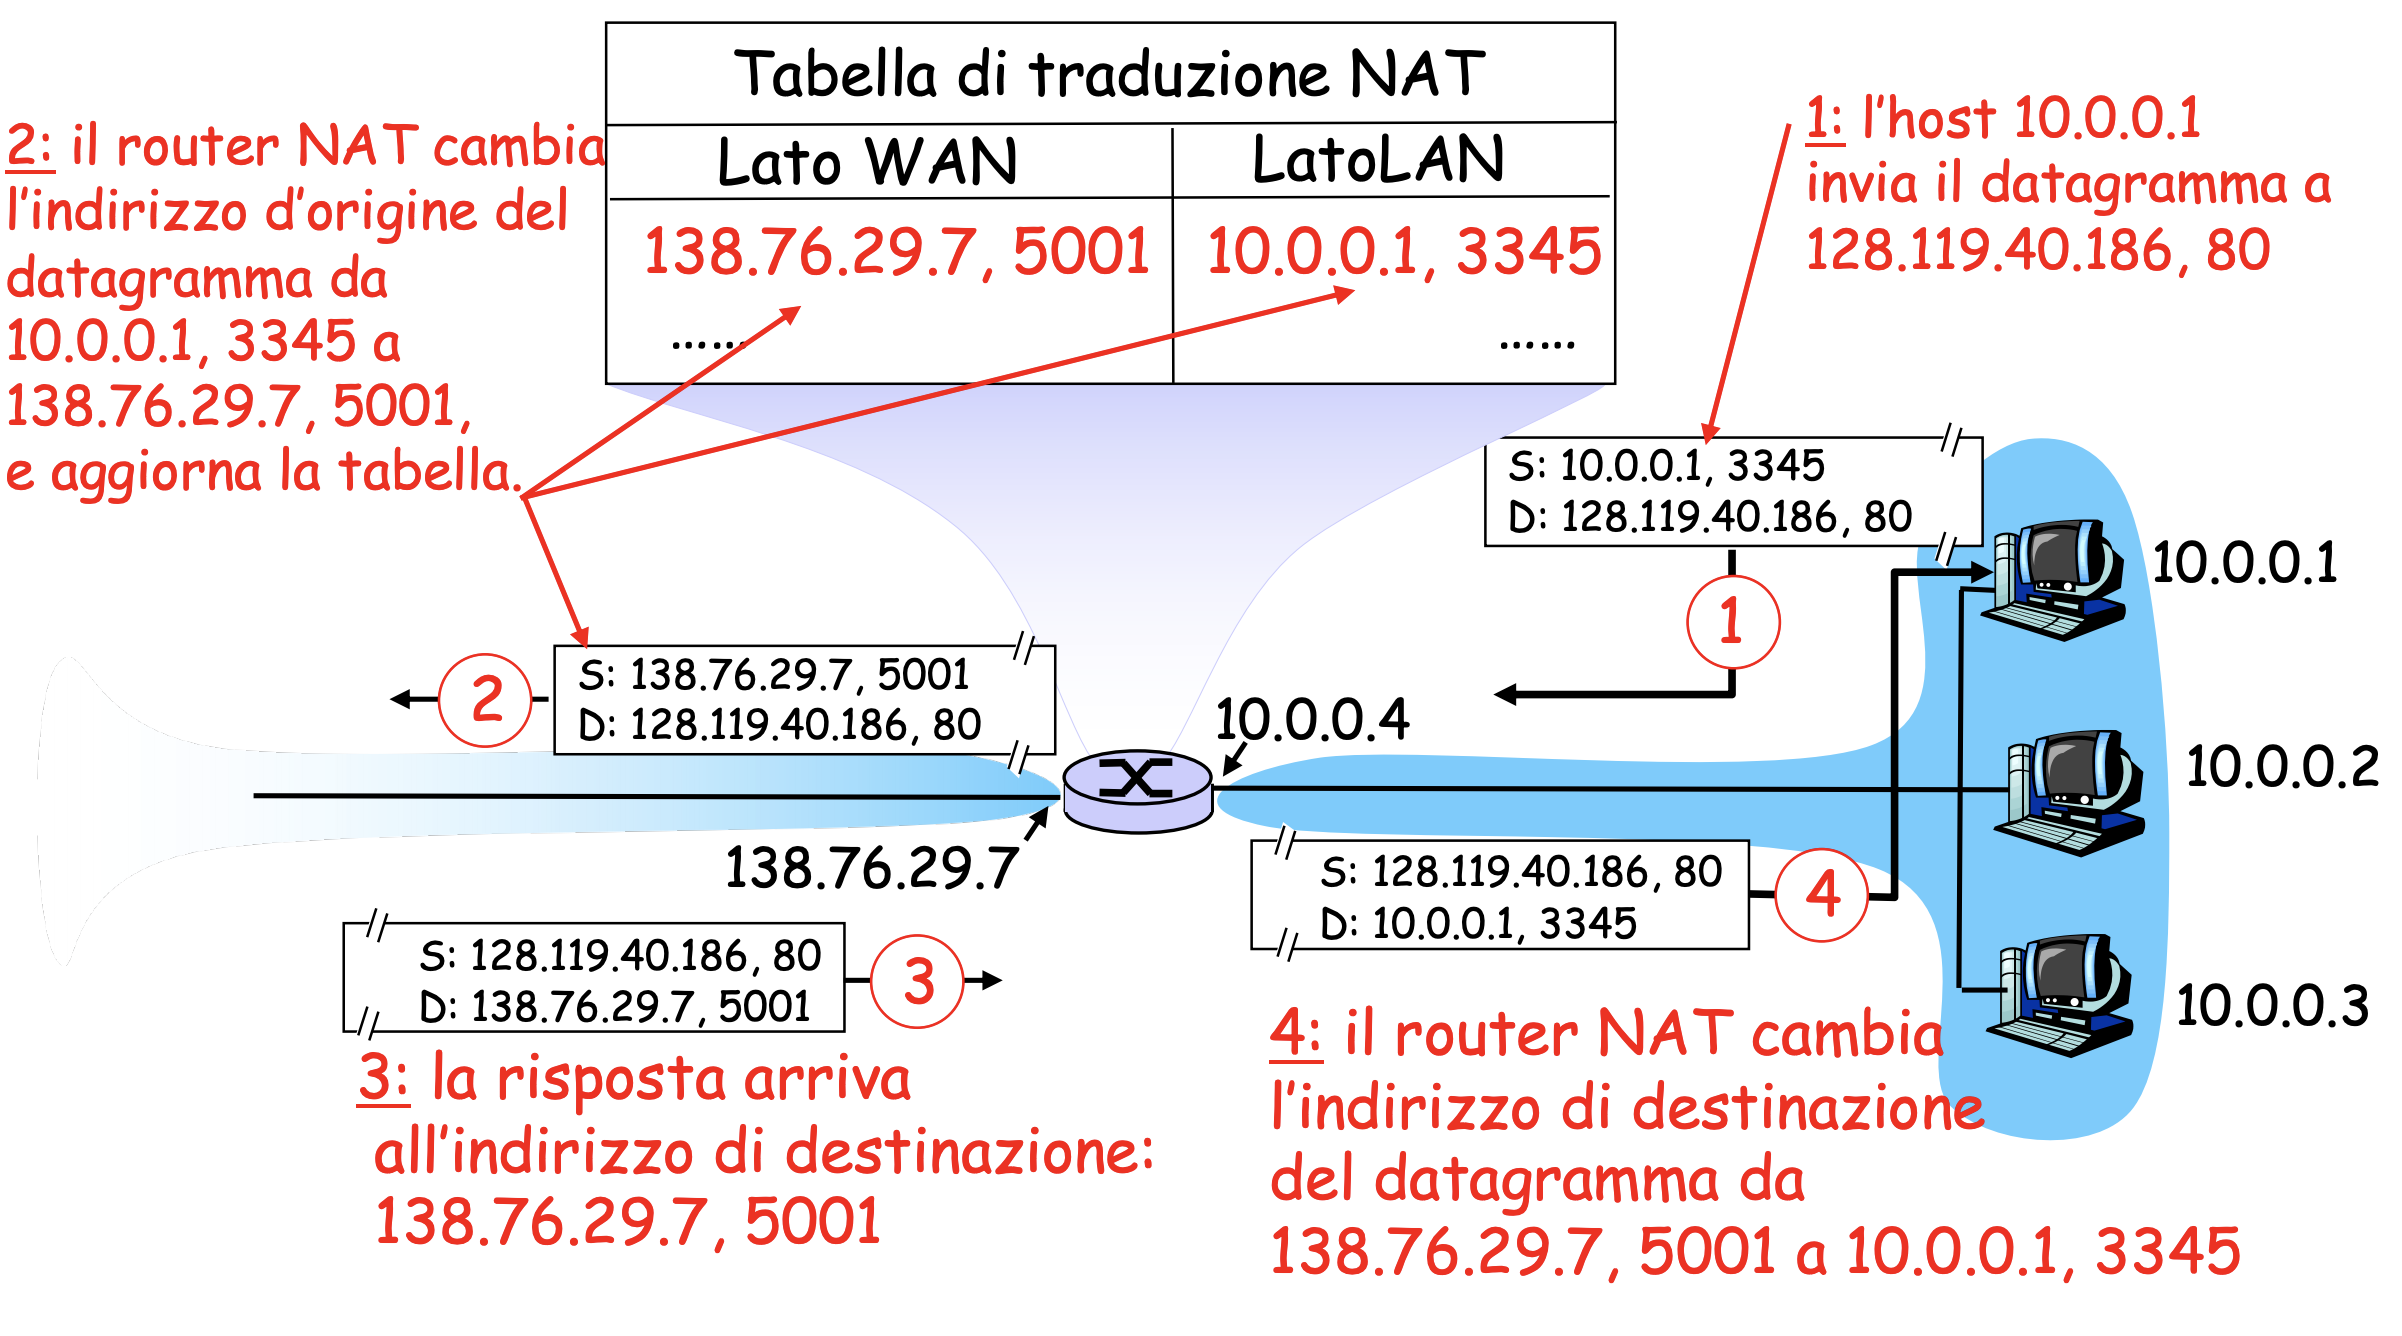
\includegraphics[width=0.7\linewidth]{nat}
	\end{center}

Il numero di porta è costituito da 16 bit, quindi sono possibili più di
60000 connessioni simultanee. NAT è contestato per diversi motivi:

\begin{itemize}
\item
  i router dovrebbero lavorare solo a livello 3+
\item
  viola il punto-punto, causando interferenze a P2P (serve una specifica
  configurazione)
\item
  si dovrebbe usare alternativamente IPv6
\end{itemize}

\hypertarget{header-n141}{%
\paragraph{Collegamenti dall'esterno}\label{header-n141}}

Un problema importante del NAT è l'impossibilità di effettuare
collegamenti dall'esterno a un host interno alla rete (come un server
web). Per effettuare questo si possono implementare alcune soluzioni

\begin{itemize}
\item
  impostare delle configurazioni statiche per inoltrare le richieste
  entranti a determinate porte dell'host (tabelle di forwarding)
\item
  utilizzare \textbf{UPnP} (Universal Plug n Play), parte integrante di
  IGD (Internet Gateway Device protocol), che consente agli host
  nascosti da un NAT di chiedere in automatico di scrivere una riga
  nella tabella di forwarding
\item
  \textbf{relay} (utilizzato da Skype), prevede un punto di riferimento
  a cui entrambi i client si collegano
\end{itemize}

\begin{center}
		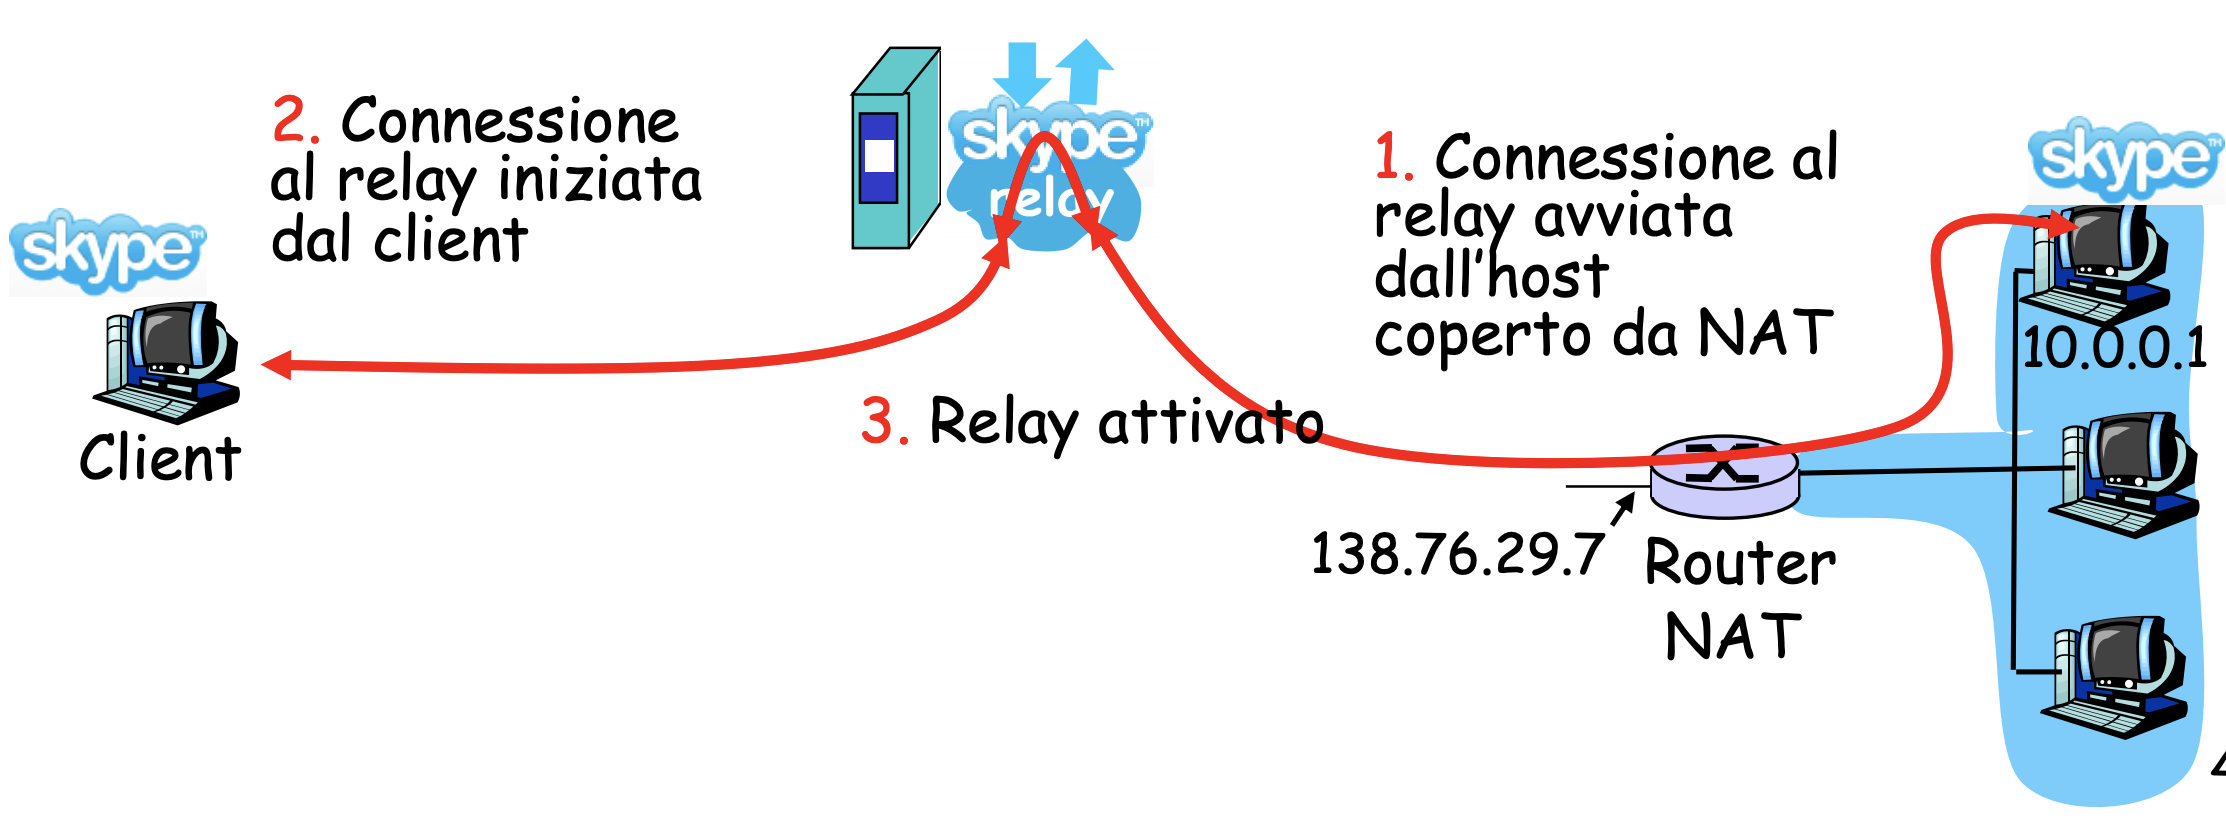
\includegraphics[width=0.7\linewidth]{skype}
	\end{center}

\hypertarget{header-n151}{%
\subsection{ICMP}\label{header-n151}}

ICMP (Internet Control Message Protocol) consente lo scambio di
informazioni relative al controllo della rete, come errori o ping. ICMP
è considerato parte di IP, i messaggi hanno un campo tipo e un campo
codice mentre l'intestazione e i primi 8 byte sono uguali al datagram
IP.

\hypertarget{header-n153}{%
\subsubsection{Traceroute e ICMP}\label{header-n153}}

Il programma invia più datagrammi con un TTL incrementale, ogni router
scarterà il datagram e invierà all'origine un'allerta ICMP la quale
calcolerà il RTT. Ogni router viene calcolato per 3 volte per avere una
media e il programma si fermerà una volta arrivato a destinazione,
ovvero quando l'host invierà un pacchetto ICMP di porta non
raggiungibile.

\hypertarget{header-n155}{%
\subsection{IPv6}\label{header-n155}}

L'esigenza principale che ha portato allo sviluppo di IPv6 è stato lo
spazio di indirizzamento IP a 32 bit che stava cominciando ad esaurirsi.
Oltre a questo, altre motivazioni erano un header più leggero per
velocizzare elaborazione e inoltro, e un agevolazione del QoS.

\hypertarget{header-n157}{%
\subsubsection{Formato dei datagrammi}\label{header-n157}}

I datagram IP sono costituiti da 40 byte di header a lunghezza fissa e
non è consentita la frammentazione.

\begin{center}
		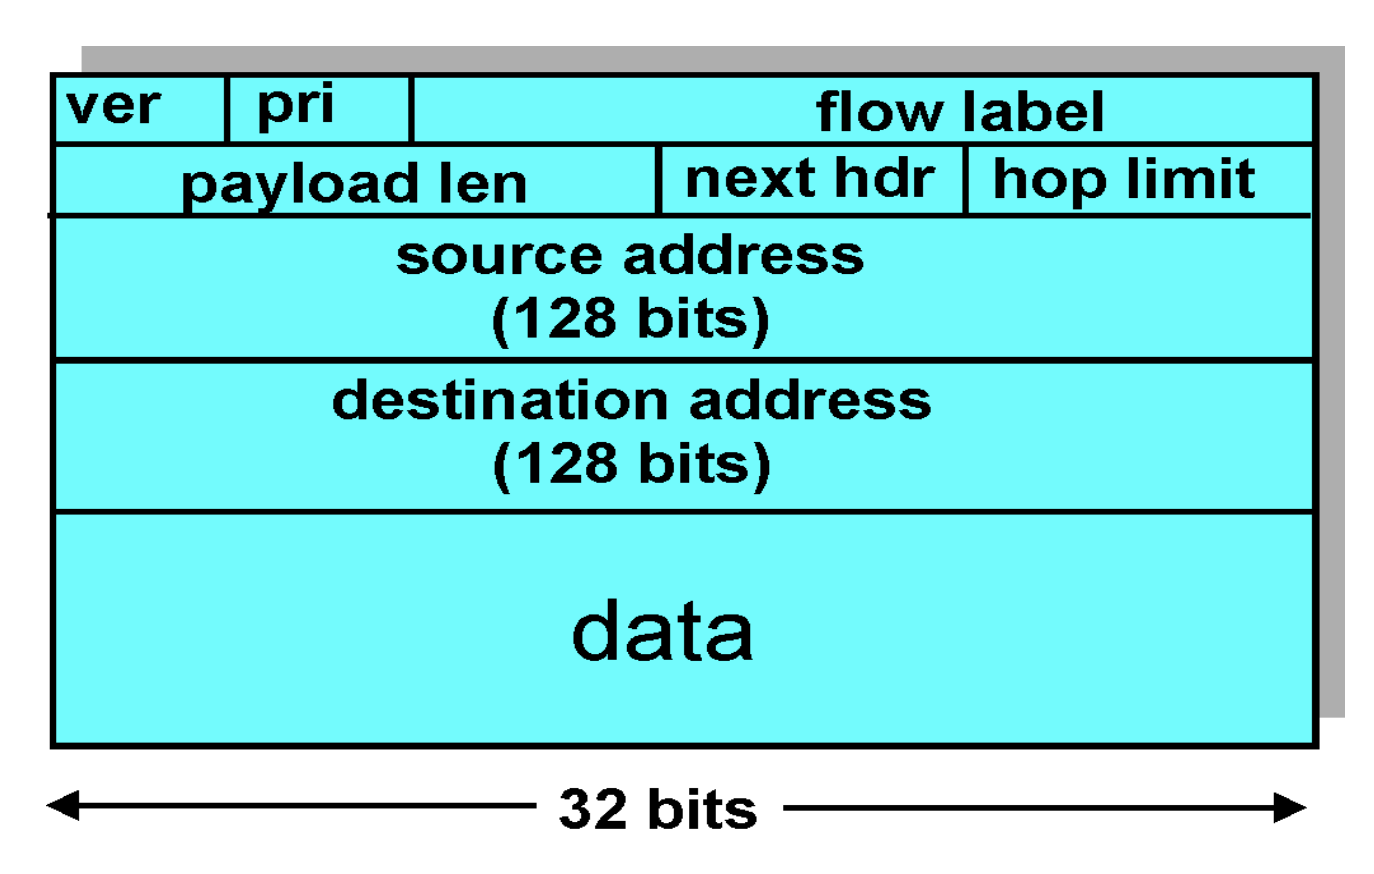
\includegraphics[width=0.7\linewidth]{ipv6}
	\end{center}

Alcuni campi nuovi sono la \textbf{priorità di flusso},
l'\textbf{etichetta di flusso} che identifica flussi particolari (non è
chiaro il concetto di flusso) e l'\textbf{intestazione successiva} che
identifica il protocollo di destinazione dei contenuti.

Inoltre, è stato rimosso il checksum poiché ridondante, il campo opzioni
non è più parte dell'intestazione ma può venire indicato in
"intestazioni successive" ed è stato introdotto \textbf{ICMPv6} con
nuovi codici che assume le funzionalità di IGMP (gestisce l'ingresso e
l'uscita di host dai gruppi multicast).

\hypertarget{header-n162}{%
\subsubsection{Passaggio a IPv6}\label{header-n162}}

Non è possibile aggiornare simultaneamente tutti i router, poiché
servirebbe stabilire una giornata "di passaggio", attualmente
impossibile. Per questo si utilizza il \textbf{tunneling}: IPv6 viene
trasportato come payload in datagram IPv4.

\begin{center}
		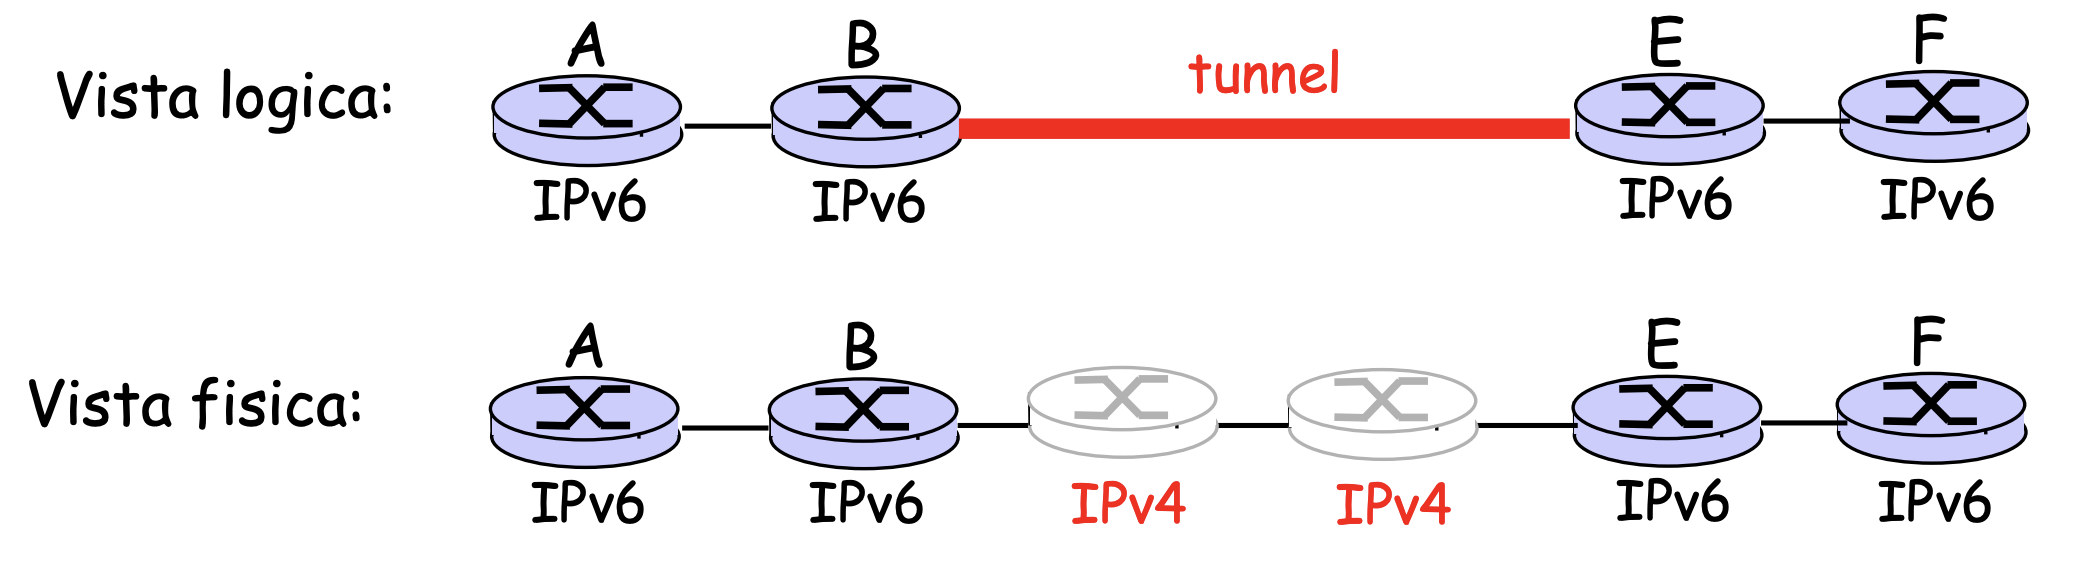
\includegraphics[width=0.7\linewidth]{tunneling}
	\end{center}

\hypertarget{header-n165}{%
\section{Algoritmi di instradamento}\label{header-n165}}

Gli algoritmi di instradamento sono implementati nelle reti a
commutazione di pacchetto, grazie all'inserimento di un valore
nell'header di livello 3, che verrà letto e confrontato con le varie
tabelle di instradamento.

\begin{wrapfigure}{r}{0.4\textwidth}
		\centering
		\vspace{-10pt}
		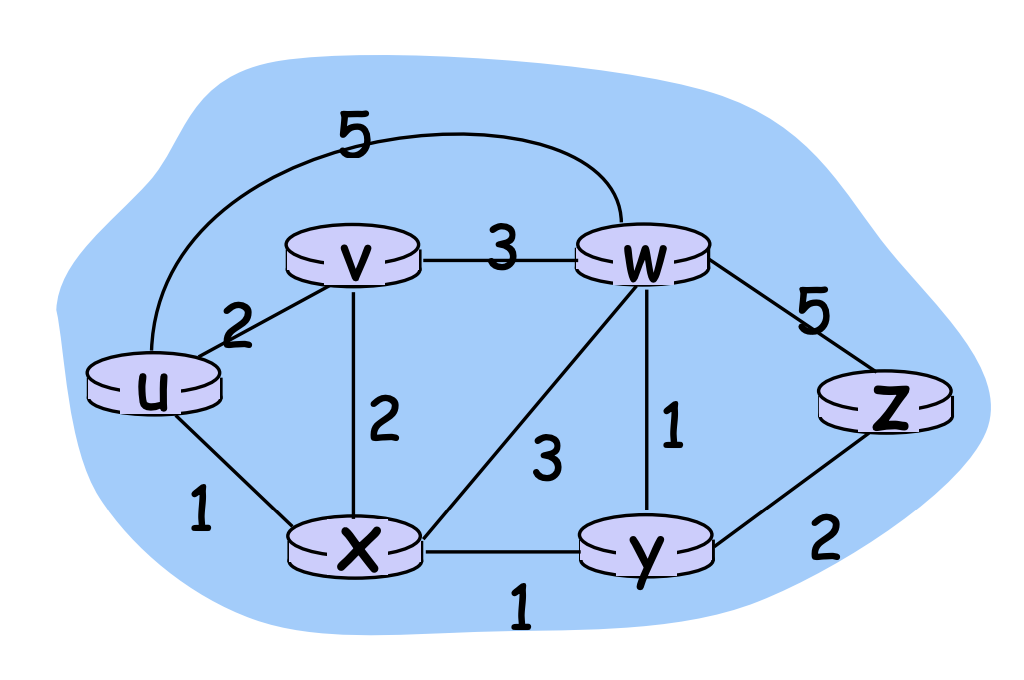
\includegraphics[width=0.4\textwidth]{grafo-rete}
		\vspace{-10pt}
	\end{wrapfigure}

Possiamo assumere una rete come un grafo dove i nodi sono i router e gli
archi sono i collegamento. Gli algoritmi di instradamento si occupano di
calcolare il cammino a costo minimo tra due router.

Questi algoritmi possono essere classificati in più modalità: globali o
decentralizzati e statici o dinamici:

\begin{itemize}
\item
  un algoritmo \textbf{globale} riceve in ingresso tutti i collegamenti
  tra nodi e loro costi, un esempio sono gli algoritmi
  \textbf{link-state}
\item
  in un algoritmo \textbf{decentralizzato} ogni nodo elabora un vettore
  di stima dei costi verso tutti gli altri nodi, quindi il cammino a
  costo minimo viene calcolato in modo distribuito e iterativo. Un
  esempio sono gli algoritmi \textbf{distance-vector}
\item
  in un algoritmo \textbf{statico} i cammini cambiano molto raramente
\item
  gli algoritmi \textbf{dinamici} determinano gli instradamenti in base
  al traffico e alla topologia della rete
\end{itemize}

\hypertarget{header-n179}{%
\subsection{Stato del collegamento (link state)}\label{header-n179}}

Un esempio di algoritmo link state è l'\textbf{algoritmo di Dijkstra} il
quale prevede che la topologia di rete e i costi siano noti a tutti i
nodi mediante il "link-state broadcast" e che tutti i nodi dispongano
delle stesse informazioni.

L'algoritmo calcola il cammino a costo minimo dall'origine a tutti gli
altri nodi, creando una \textbf{tabella d'inoltro} per quel nodo.
Essendo iterativo, dopo la k-esima iterazione i cammini a costo minimo
sono noti a k nodi di destinazione.

I costi di ogni collegamento possono essere:

\begin{itemize}
\item
  predefiniti dal provider
\item
  tutti uguali
\item
  costi effettivi (satellite)
\item
  definiti dal ritardo di collegamento
\end{itemize}

La regola è evitare che i costi dipendano dal routing.

La sua complessità con n nodi è data da

\[O(nlogn)\]

Può presentare delle oscillazioni ad esempio nel costo del collegamento
in base alla quantità di traffico trasportato.

\hypertarget{header-n196}{%
\subsection{Algoritmo con vettore distanza}\label{header-n196}}

Un esempio di algoritmo con vettore distanza è la \textbf{formula di
Bellman-Ford} (o a programmazione dinamica) che definisce il costo del
percorso a costo minimo da x a y

\[d_x(y) = min_v\{c(x,v) + d_v(y)\}\]

dove min\emph{v riguarda tutti i vicini di x, c(x,v) comprende il costo
di tutti i collegamenti diretti da x a v e d}v(y) è il percorso a costo
minimo da v a y.

L'algoritmo viene eseguito nel modo seguente: il nodo x contatta tutti i
vicini v e si fa dare da ognuno di essi ogni costo per andare a y,
successivamente valuterà tutte le alternative.

L'idea di base è che ogni nodo invia una copia del proprio vettore
distanza a ogni vicino, quando un nodo riceve un nuovo vettore distanza
da un vicinolo salva e usa la formula B-F per aggiornare il proprio DV.
Finché tutti i nodi continuano a cambiare i propri DV in maniera
asincrona, ciascuma stima Dx(y) coverge a d\_x(y).

L'algoritmo con vettore distanza è \textbf{iterativo ed asincrono},
poiché ogni iterazione locale è causata dal cambio del costo di un link
locale o dalla ricezione di un DV aggiornato; è \textbf{distribuito}
poiché ogni nodo aggiorna i suoi vicini solo quando il suo DV cambia.

\hypertarget{header-n203}{%
\subsubsection{Modifica dei costi}\label{header-n203}}

Quando un nodo rileva un cambiamento nel costo dei collegamenti allora
aggiorna il proprio vettore distanza e lo trasmetterà ai suoi vicini,
secondo il principio che "le buone notizie viaggiano in fretta".

\hypertarget{header-n205}{%
\subsubsection{Confronto tra algoritmi LS e DV}\label{header-n205}}

\begin{itemize}
\item
  Complessità dei messaggi

  \begin{itemize}
  \item
    LS con n nodi, E collegamenti implica l'invio di O(nE) messaggi
  \item
    DV richiede scambi tra nodi adiacenti, quindi il tempo di
    convergenza può variare
  \end{itemize}
\item
  Velocità di convergenza

  \begin{itemize}
  \item
    LS: l'algoritmo O(n2) richiede O(nE) messaggi, ci possono essere
    oscillazioni di velocità
  \item
    DV può convergere lentamente, può presentare cicli d'instradamento e
    può presentare il problema del conteggio all'infinito
  \end{itemize}
\item
  \textbf{Robustezza:} cosa avviense se un router funziona male

  \begin{itemize}
  \item
    LS: un router può comunicare via broadcast un costo sbagliato per
    uno dei suoi collegamenti (non per altri), i nodi si occupano di
    calcolare solo le proprie tabelle
  \item
    DV: un nodo può comunicare cammini a costo minimo errati a tutte le
    destinazioni, la tabella di ogni nodo può essere usata da altri
    quindi \underline{un calcolo errato si diffonde per l'intera rete}
  \end{itemize}
\end{itemize}

\hypertarget{header-n228}{%
\subsection{Instradamento gerarchico}\label{header-n228}}

Fino ad ora abbiamo visto la rete come un insieme di router
interconnessi, con una visione omogenea, ma nella pratica le cose non
sono così semplici. Nella realtà ci sono 200 milioni di destinazioni,
quindi archiviare tutte le informazioni di instradamento su ogni host
sarebbe impossibile data l'enorme quantità di memoria necessaria e
l'elevato traffico (bloccherebbe il resto) che si creerebbe.

Per questo, conviene impostare la rete Internet con una
\textbf{autonomia amministrativa}, secondo la quale idealmente ciascuno
sarebbe in grado di amministrare la propria rete connettendola alle
altre.

Nella realtà è possibile organizzare i router in \textbf{sistemi
autonomi} (AS), dove in ogni gruppo autonomo i router eseguono lo stesso
algoritmo di instradamento (protocollo \textbf{intra-AS}) mentre i
\textbf{router gateway} hanno il compito di inoltrare i pacchetti a
destinazioni esterne.

Ogni sistema autonomo sa come inoltrare i pacchetti lungo il percorso
ottimo verso qualsiasi destinazione interna al gruppo, mentre per
trasferire dati tra sistemi autonomi differenti (i quali potrebbero
usare protocolli differenti) si utilizza l'instradamento
\textbf{inter-AS}.

\begin{center}
		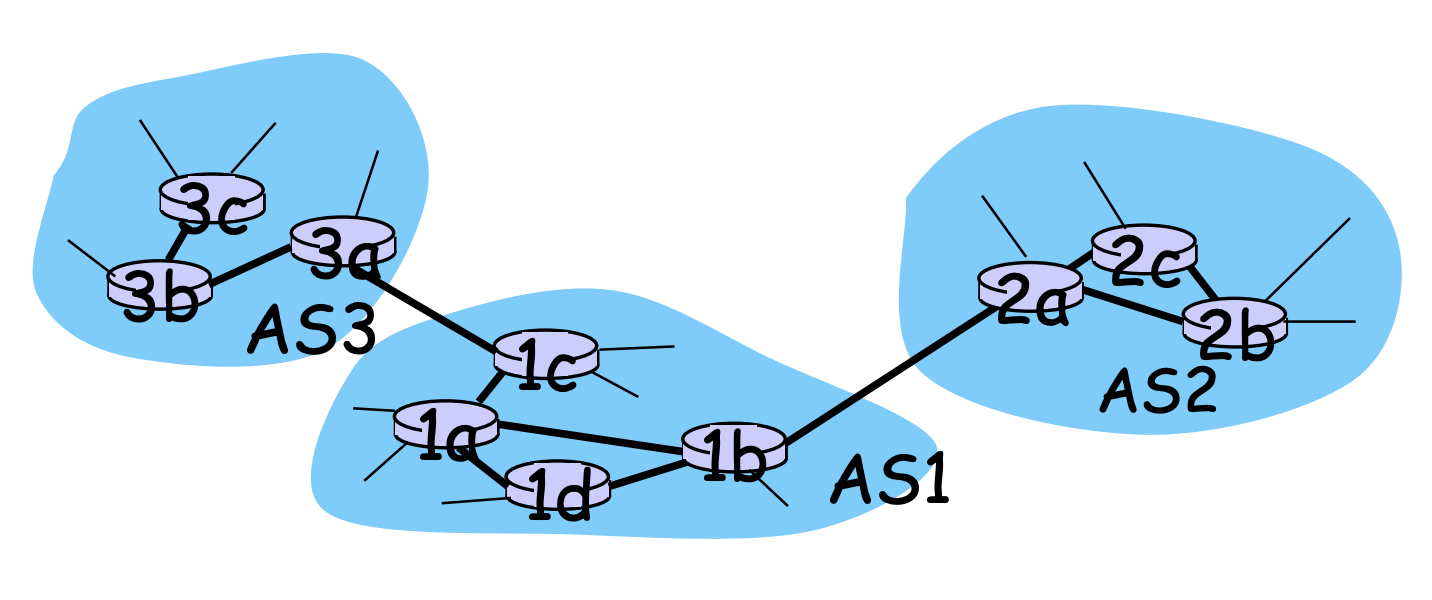
\includegraphics[width=0.7\linewidth]{as}
	\end{center}

\begin{center}
		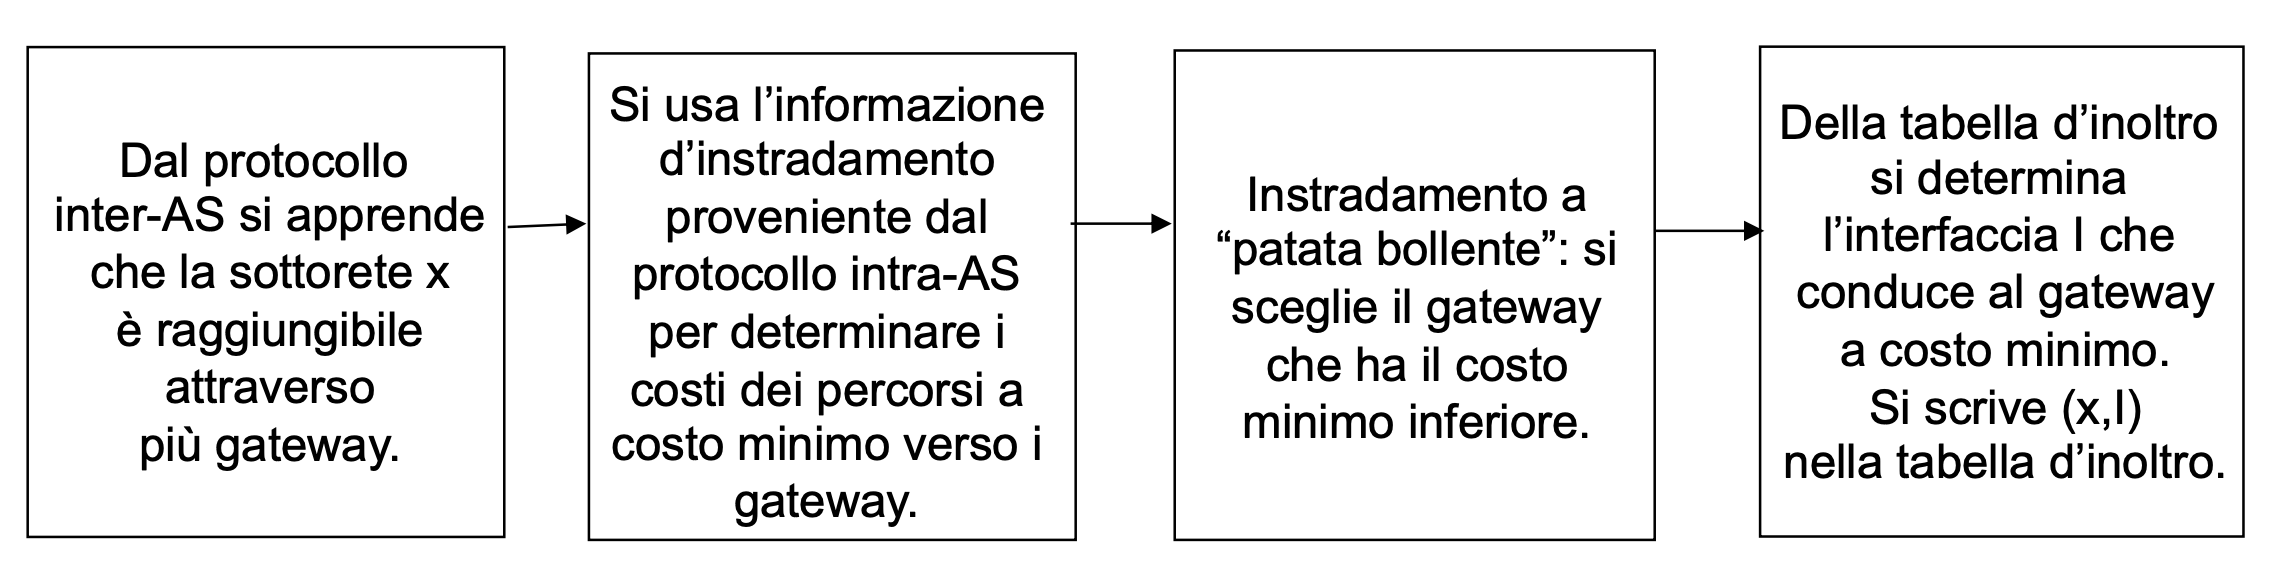
\includegraphics[width=0.7\linewidth]{routing-as}
	\end{center}

\hypertarget{header-n235}{%
\section{Instradamento in Internet}\label{header-n235}}

I protocolli d'instradamento \emph{intra-AS} sono noti come protocolli
gateway interni (\textbf{IGP}), i più comuni sono:

\begin{itemize}
\item
  \textbf{RIP}: Routing Information Protocol
\item
  \textbf{OSPF}: Open Shortest Path First
\item
  \textbf{IGRP}: Interior Gateway Routing Protocol (proprietario Cisco)
\end{itemize}

\hypertarget{header-n244}{%
\subsection{RIP (Routing Information Protocol)}\label{header-n244}}

RIP è un protocollo a vettore distanza incluso in UNIX BSD dagli anni
'80. Effettua un conteggio degli hop come metrica di costo con un
massimo di 15 hop.

I router adiacenti si scambiano aggiornamenti ogni 30 secondi mediante
l'annuncio RIP (\emph{RIP advertisement}), contenente un elenco di fino
a 25 sottoreti di destinazione interne all'AS, insieme alla distanza tra
il mittente ed esse.

Se un router non riceve notizie dal vicino per più di 180 secondi il
nodo viene considerato spento, con il ricalcolo della tabella e la
propagazione dell'informazione agli altri vicini. L'utilizzo
dell'\emph{inversione avvelenata} evita i loop (16 hop).

RIP viene implementato a livello applicazione con messaggi su socket
standard e protocollo di trasporto standard.

\hypertarget{header-n249}{%
\subsection{OSPF (Open Shortest Path First)}\label{header-n249}}

Essendo open, le specifiche del protocollo sono pubblicamente
disponibili. Protocollo a link-state, utilizza il flooding di
informazioni di stato del link e l'algoritmo di Dijkstra per determinare
il percorso a costo minimo. Ogni volta che si verifica un cambiamento su
un link il router inoltra l'informazione a tutti i router (all'intero
AS) utilizzando il flooding, i messaggi sono trasportati da IP.

OSPF presenta alcuni vantaggi rispetto a RIP:

\begin{itemize}
\item
  \textbf{sicurezza}: scambi tra router autenticati
\item
  \textbf{multipath}: consente l'utilizzo di più percorsi con uguale
  costo
\item
  per ogni link possono esserci più costi in base al servizio (es.
  satellite costo elevato)
\item
  \textbf{supporto unicast e multicast}: viene utilizzato OSPF Multicast
\item
  \textbf{supporto alle gerarchie} in un dominio d'instradamento
\end{itemize}

\hypertarget{header-n263}{%
\subsubsection{OSPF strutturato gerarchicamente}\label{header-n263}}

\begin{center}
		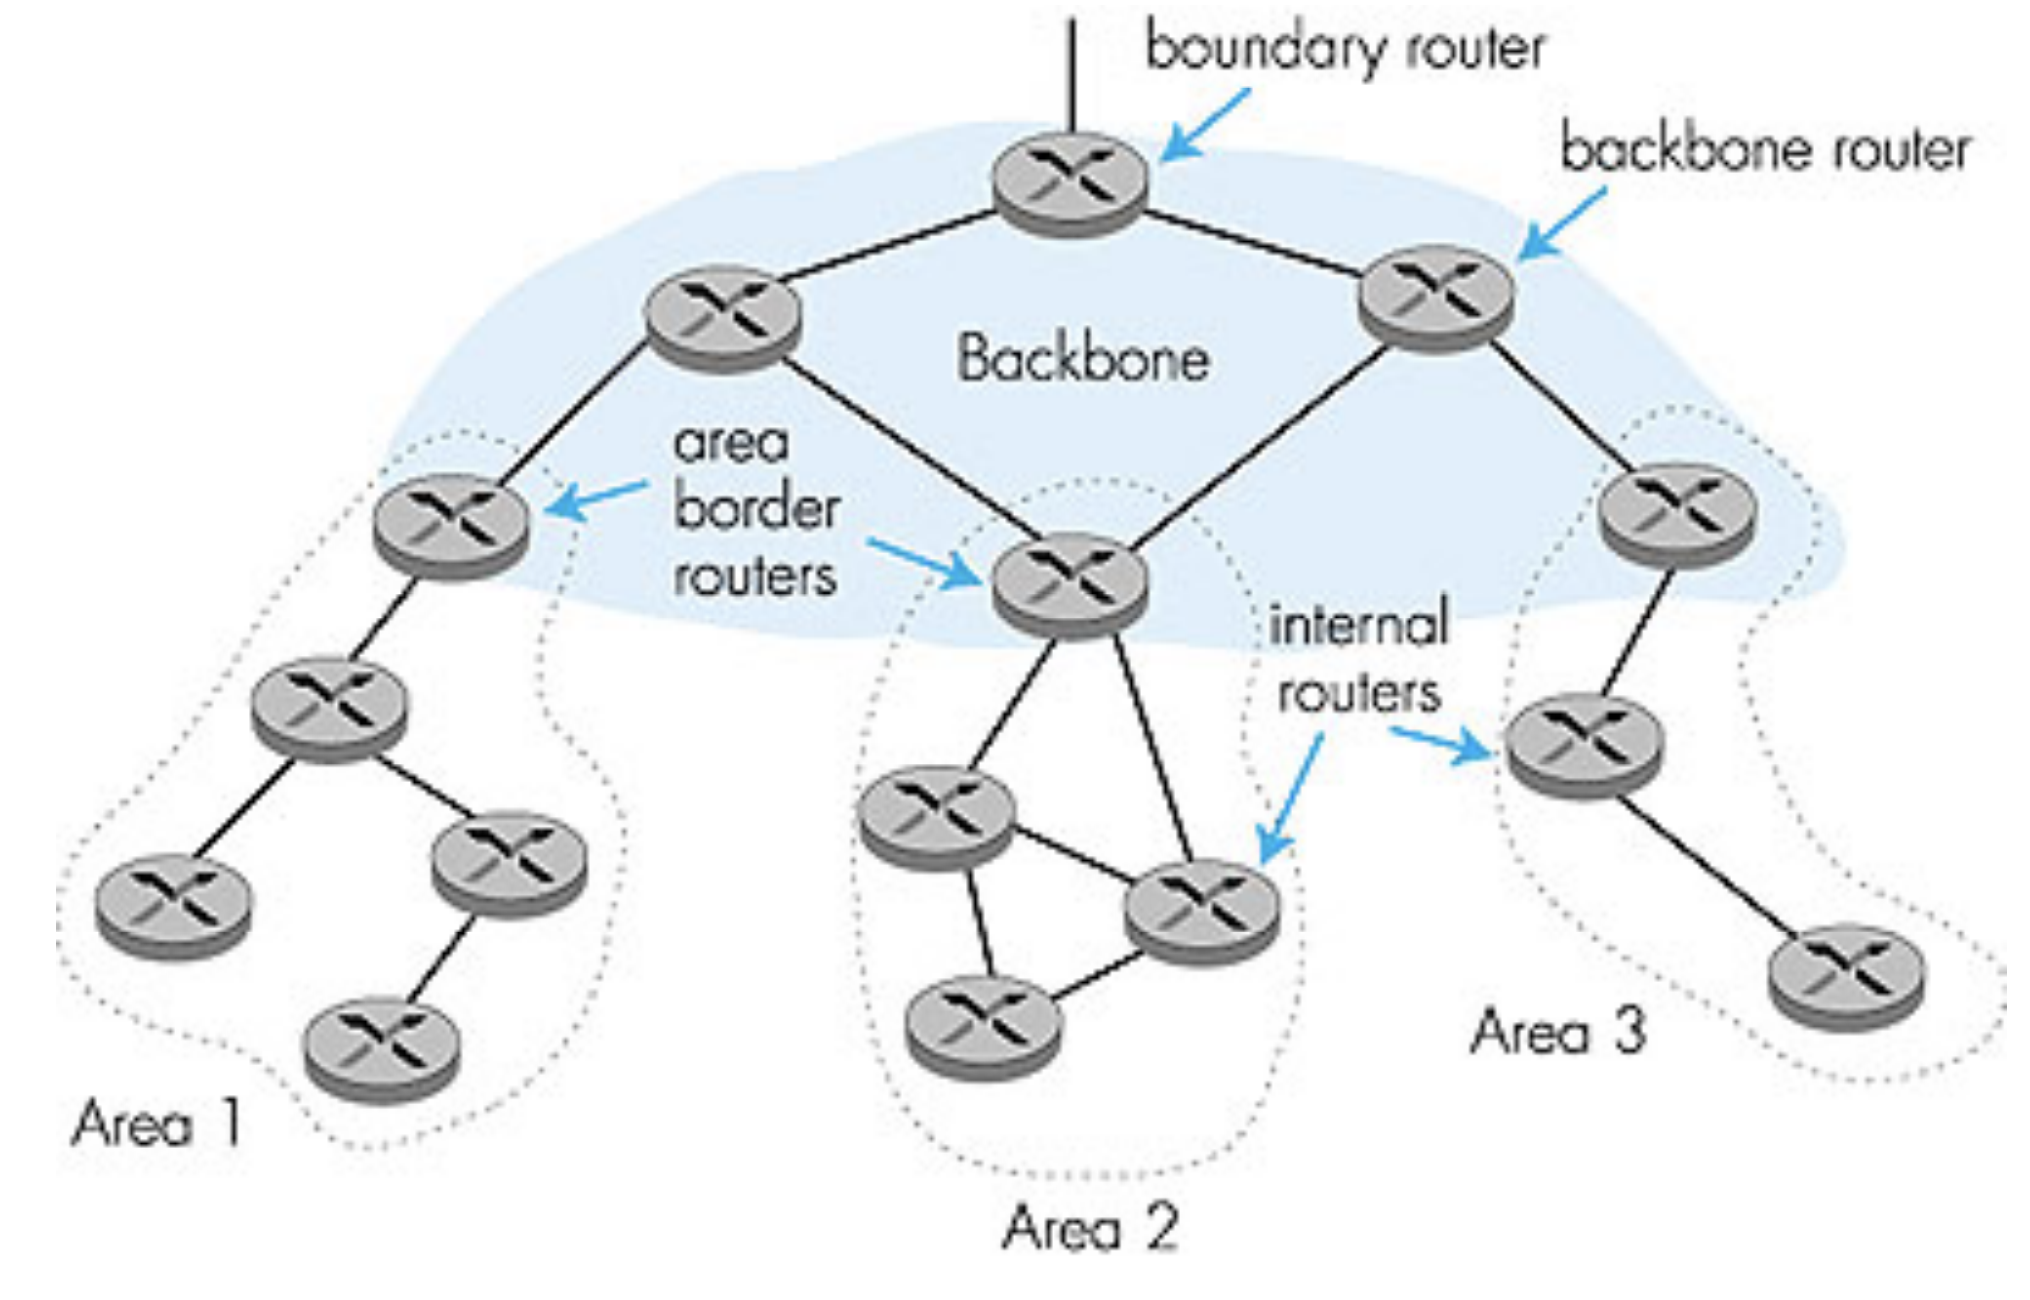
\includegraphics[width=0.7\linewidth]{ospf-gerarchia}
	\end{center}

La struttura gerarchica in OSPF consente di impostare due livelli: area
locale e dorsale, nelle quali i messaggi LS sono solo all'interno
dell'area e ogni nodo conosce la direzione verso le reti nelle altre
aree.

I \textbf{router di confine d'area} appartengono sia alla dorsale che a
un'area generica, i \textbf{router di dorsale} effettuano
l'instradamento interno alla dorsale, i \textbf{router di confine}
scambiano informazioni con router di altri AS.

\hypertarget{header-n267}{%
\subsection{BGP: instradamento inter-AS}\label{header-n267}}

Il protocollo BGP (Border Gateway Protocol) è l'attuale standard
\emph{de facto} per l'instradamento inter-AS, che mette a disposizione
di ciascun AS le seguenti funzionalità:

\begin{enumerate}
\def\labelenumi{\arabic{enumi}.}
\item
  ottenere informazioni sulla raggiungibilità delle sottoreti da parte
  di AS confinanti
\item
  propagare le informazioni di raggiungibilità a tutti i router interni
  di un AS
\item
  determinare percorsi "buoni" verso le sottoreti sulla base delle
  informazioni di raggiungibilità e delle politiche dell'AS
\end{enumerate}

In breve, BGP consente alle sottoreti di comunicare la propria esistenza
alla rete Internet.

\hypertarget{header-n280}{%
\subsubsection{Fondamenti di BGP}\label{header-n280}}

Due router che si scambiano messaggi BGP sono chiamati \textbf{peer BGP}
mentre la connessione TCP è detta \textbf{sessione BGP}. Quando un AS
annuncia un prefisso ad un altro AS, sta in realtà "promettendo" di
inoltrare i datagrammi sul prefisso stabilito, un AS può aggregare più
prefissi in un annuncio.

\begin{center}
		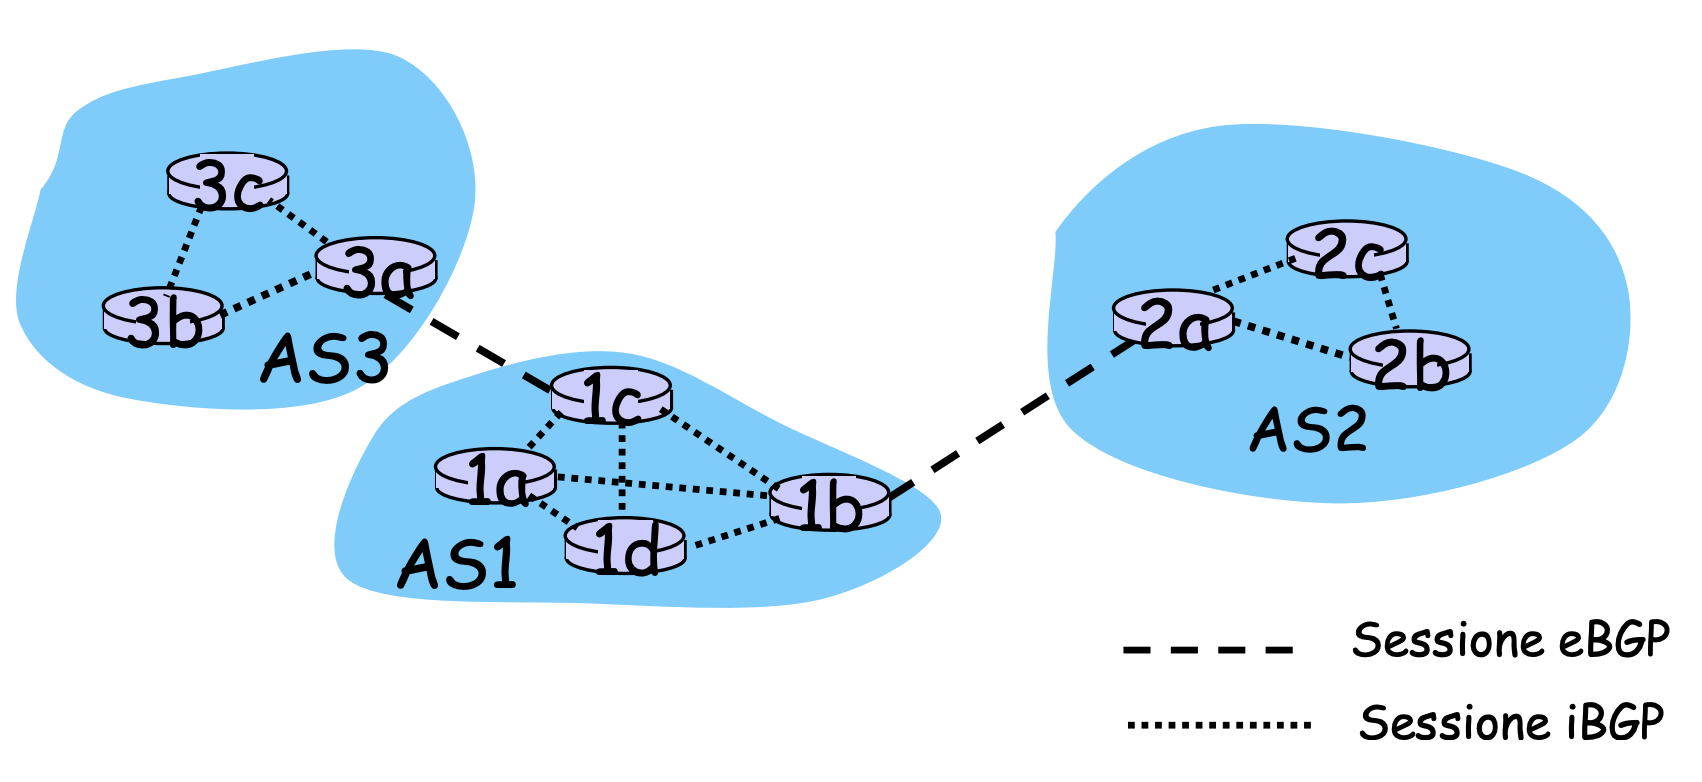
\includegraphics[width=0.7\linewidth]{bgp}
	\end{center}

Le sessioni BGP interne sono utilizzate per distribuire i prefissi a
tutti i router del AS, mentre le sessioni esterne scambiano informazioni
sulla raggiungibilità dei prefissi.

\hypertarget{header-n328}{%
\paragraph{Attributi del percorso}\label{header-n328}}

Quando viene annunciato un prefisso, nel messaggio vengono aggiunti
anche degli attributi BGP come:

\begin{itemize}
\item
  \textbf{AS-PATH} che elenca gli AS che ha attraversato l'annuncio
\item
  \textbf{NEXT-HOP} che indica l'eventuale collegamento fisico su cui
  viene inoltrato il pacchetto
\end{itemize}

Ogni router gateway ha delle \textbf{politiche di importazione} per
decidere se accettare o filtrare la rotta.

\begin{center}
		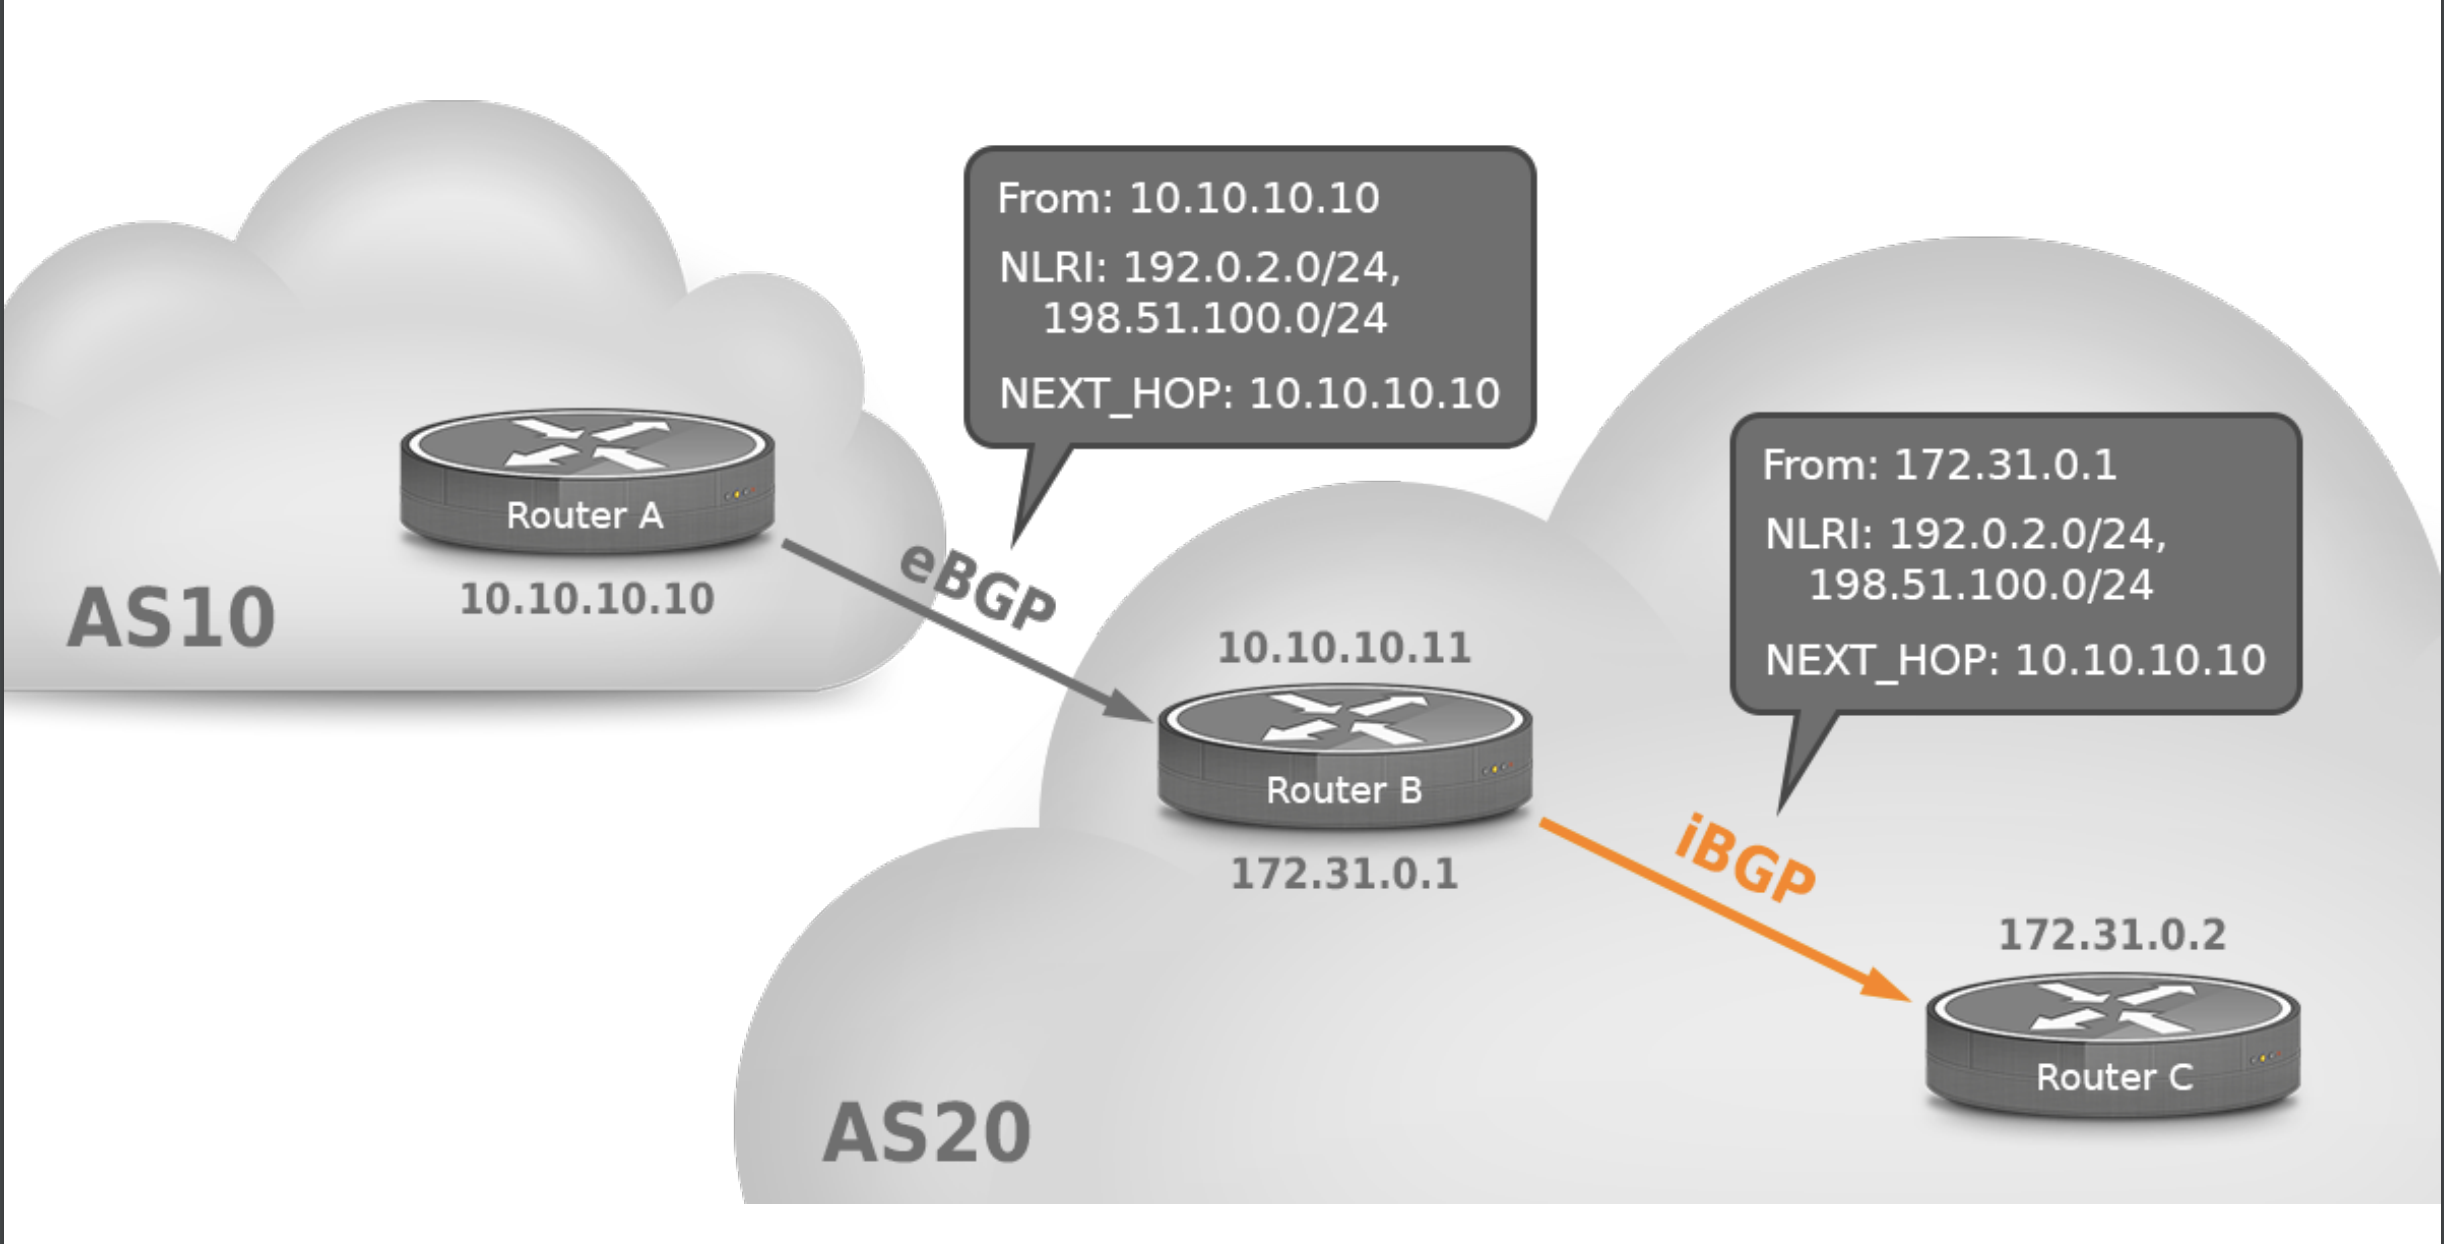
\includegraphics[width=0.7\linewidth]{next-hop}
	\end{center}

\hypertarget{header-n330}{%
\paragraph{Selezione dei percorsi}\label{header-n330}}

Nel caso in cui siano presenti più rotte si seguono alcune regole di
eliminazione:

\begin{enumerate}
\def\labelenumi{\arabic{enumi}.}
\item
  si preferiscono le rotte con dei valori di preferenza locale più alti
\item
  si seleziona la rotta con AS-PATH più breve
\item
  si seleziona la rotta con il router NEXT-HOP più vicino, instradamento
  a \emph{patata bollente}
\item
  se avanzano più rotte, ci si basa sugli identificatori BGP
\end{enumerate}

\hypertarget{header-n327}{%
\paragraph{Messaggi BGP}\label{header-n327}}

\begin{itemize}
\item
  \textbf{OPEN}: apre la connessione TCP e autentica il mittente
\item
  \textbf{UPDATE}: annuncia il nuovo percorso
\item
  \textbf{KEEPALIVE}: mantiene la connessione attiva in mancanza di
  UPDATE
\item
  \textbf{NOTIFICATION}: riporta gli errori del precedente messaggio;
  usato anche per chiudere il collegamento.
\end{itemize}

\hypertarget{header-n349}{%
\subsubsection{Differenze tra i protocolli inter-AS e
intra-AS}\label{header-n349}}

\begin{itemize}
\item
  \textbf{Politiche}

  \begin{itemize}
  \item
    Inter-AS: l'amministrazione vuole controllare l'instradamento del
    traffico e chi instrada attraverso le sue reti
  \item
    Intra-AS: un solo controllo amministrativo, rotte interne scelta
    senza questioni di politica importanti
  \end{itemize}
\item
  \textbf{Scala}: l'instradamento gerarchico fa risparmiare sulle
  tabelle d'instradamento riducendo il traffico di aggiornamento
\item
  \textbf{Prestazioni}: Intra-AS orientato alle prestazioni, Inter-AS le
  politiche possono prevalere sulle prestazioni
\end{itemize}
	
	\chapter{Il livello di collegamento}
	
	\hypertarget{header-n0}{%
\section{Livello di collegamento: introduzione e
servizi}\label{header-n0}}

A livello di collegamento definiamo come \textbf{nodi} host e router,
che vengono collegati tra loro da \textbf{collegamenti (link)} di
tipologia cablata, wireless o LAN. Le unità di dati scambiate a livello
link sono chiamate \textbf{frame}.

In breve, i protocolli a livello di collegamento si occupano del
trasporto di datagram lungo un singolo canale di comunicazione. Questi
protocolli possono essere differenti sui vari collegamenti che seguirà
il datagram e i servizi erogati possono essere differenti: non tutti i
protocolli, ad esempio, forniscono consegna affidabile.
\hypertarget{header-n4}{%
\subsection{Servizi offerti a livello di link}\label{header-n4}}

\begin{itemize}
\item
  \textbf{Framing}

  \begin{itemize}
  \item
    I protocolli incapsulano i datagram del livello di rete in frame a
    livello di link
  \item
    Il protocollo MAC controlla l'accesso al mezzo trasmissivo (il
    collegamento)
  \item
    Viene utilizzato l'indirizzo MAC (diverso dall'IP) per identificare
    i nodi di origine e destinazione
  \end{itemize}
\item
  \textbf{Consegna affidabile}

  \begin{itemize}
  \item
    Non necessaria sui collegamenti a basso numero di errori sui bit
    (fibra ottica, cavo coassiale, doppino intrecciato)
  \item
    Utilizzata nei collegamenti soggetti a elevato tasso di errori
    (wireless)
  \end{itemize}
\item
  \textbf{Controllo di flusso:} non saturare il nodo ricevente
\item
  \textbf{Rilevazione degli errori:} causati dall'attenuazione del
  segnale e dal rumore elettromagnetico, il ricevente individua gli
  errori grazie a un bit di controllo inserito nel frame
\item
  \textbf{Correzione degli errori:} il ricevente determina l'errore e lo
  corregge
\item
  \textbf{Half-duplex e full-duplex}
\end{itemize}

\hypertarget{header-n30}{%
\subsection{Dov'è implementato il livello link}\label{header-n30}}

Viene implementato in tutti gli host grazie ad un adattatore (o
\textbf{NIC}, network interface card) che implementa il livello di
collegamento e fisico ed è una combinazione di hardware, software e
firmware.

L'adattatore ha il ruolo in trasmissione di incapsulare i datagram nei
frame impostando bit di controllo errori, trasferimento affidabile,
controllo di flusso, ecc e dall'altro lato di individuare errori ed
estrarre i datagram passandoli al nodo.

\hypertarget{header-n33}{%
\section{Tecniche di rilevazione e correzione degli
errori}\label{header-n33}}

La rilevazione degli errori non è attendibile al 100\%, infatti è
possibile che ci siano errori non rilevati e per ridurre che questo
accada le tecniche più sofisticate prevedono un'elevata ridondanza.

\hypertarget{header-n35}{%
\subsection{Controllo di parità}\label{header-n35}}

Nel caso di \textbf{unico bit di parità} è presente un solo bit che
consente di riconoscere che si è verificato almeno un errore in un bit.

Nel caso della \textbf{parità bidimensionale} è possibile individuare e
correggere il bit alterato.

\begin{center}
	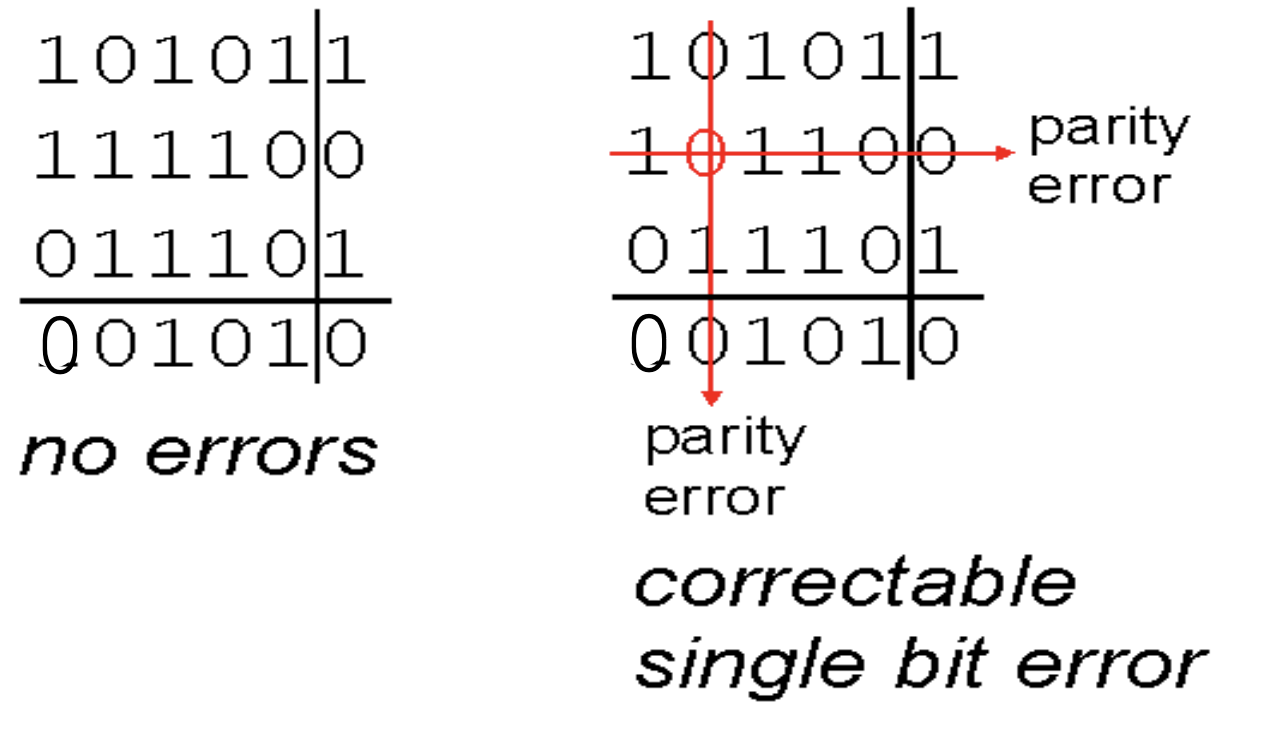
\includegraphics[width=0.7\linewidth]{parita-2d.png}
\end{center}

\hypertarget{header-n39}{%
\section{Protocolli di accesso multiplo}\label{header-n39}}

Esistono due tipi di collegamenti di rete:

\begin{itemize}
\item
  collegamento \textbf{punto-punto} (PPP), utilizzato per connessioni
  telefoniche o collegamenti punto-punto tra Ethernet e host
\item
  collegamento \textbf{broadcast} (cavo o canale condiviso) come
  l'Ethernet tradizionale o wireless
\end{itemize}

Nel caso di una connessione a un canale broadcast condiviso è consentita
la connessione anche a migliaia di nodi: si genera quindi una
\textbf{collisione} quando i nodi ricevono più di un frame
contemporaneamente.

I protocolli ad accesso multiplo consentono quindi di definire le
modalità con cui i nodi regolano le loro trasmissioni sul canale, la cui
comunicazione utilizza il canale stesso (non è presente un canale fuori
banda).

Il protocollo di accesso multiplo ideale sarebbe un protocollo
decentralizzato e semplice che suddivide il tasso trasmissivo tra il
numero di nodi che devono inviare dati. Ovviamente tale protocollo non è
possibile

I protocolli di accesso multiplo esistenti vengono classificati come
segue:

\begin{itemize}
\item
  Protocolli a \textbf{suddivisione del canale}: il canale è suddiviso
  in parti (slot di tempo, frequenza, codice) ed allocate a uno
  specifico nodo per utilizzo esclusivo
\item
  Protocolli ad \textbf{accesso casuale}: nessuna divisione, si possono
  verificare collisioni, i nodi ritrasmettono ripetutamente i pacchetti
\item
  Protocolli a \textbf{rotazione}: ogni nodo ha il suo turno di
  trasmissione, ma quelli che hanno molto da trasmettere potrebbero
  avere turni più lunghi
\end{itemize}

\hypertarget{header-n57}{%
\subsection{Protocolli a suddivisione del canale}\label{header-n57}}

\hypertarget{header-n58}{%
\subsubsection{TDMA: accesso multiplo a divisione di
tempo}\label{header-n58}}

Il protocollo TDMA consiste in turni per accedere al canale,
suddividendolo in intervalli di tempo. Gli slot non usati rimangono
inattivi.

\begin{center}
		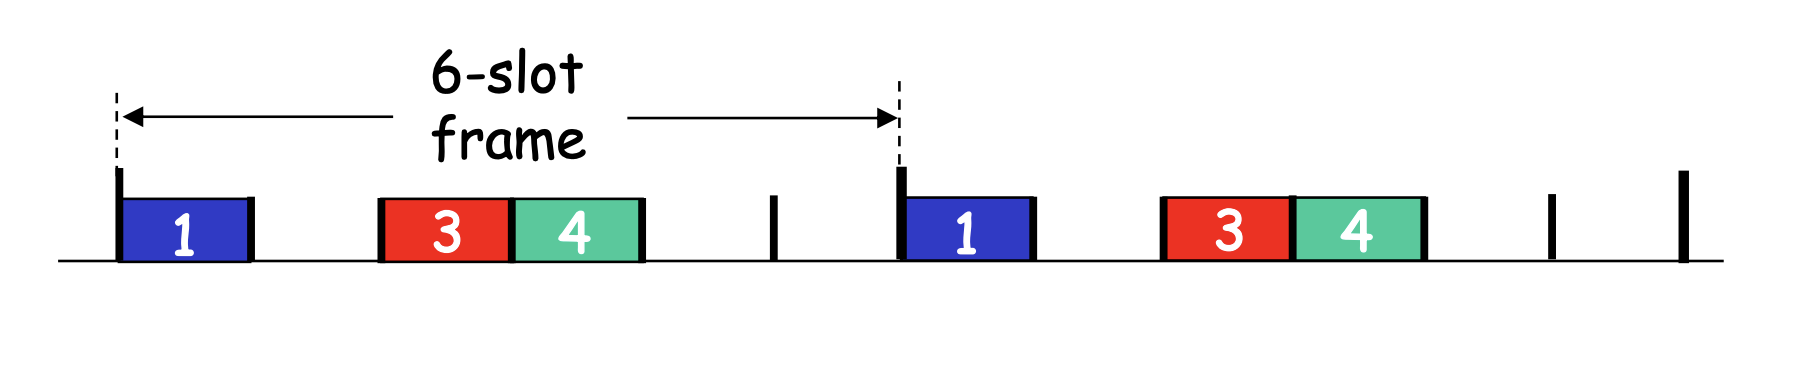
\includegraphics[width=0.7\linewidth]{tdma}
	\end{center}

\hypertarget{header-n61}{%
\subsubsection{FDMA: accesso multiplo a divisione di
frequenza}\label{header-n61}}

Il protocollo FDMA suddivide il canale in bande di frequenza e ad ogni
nodo viene assegnata una banda di frequenza prefissata.

\begin{center}
		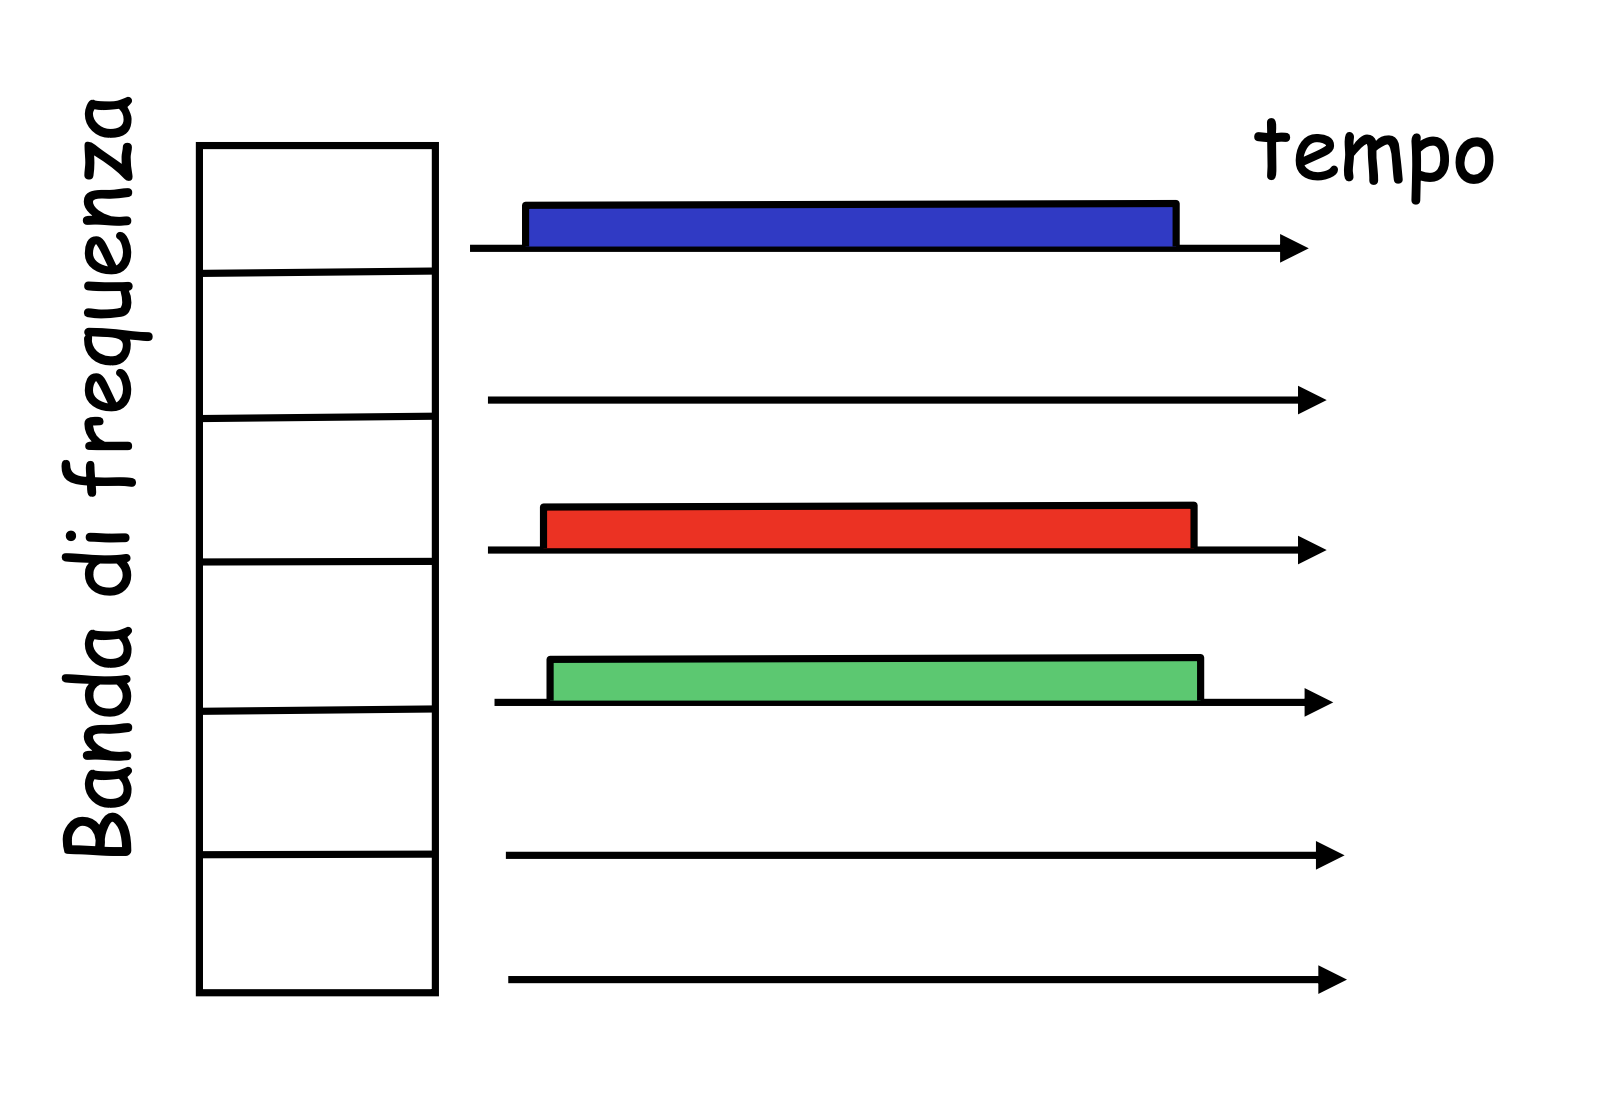
\includegraphics[width=0.7\linewidth]{fdma}
	\end{center}

\hypertarget{header-n64}{%
\subsection{Protocolli ad accesso casuale}\label{header-n64}}

Nei protocolli ad accesso casuale ogni nodo che deve inviare dati
trasmette alla massima velocità consentita dal canale, senza
coordinazione tra i nodi. Se più nodi stanno trasmettendo si verifica
una collisione. Il protocollo definisce quindi come rilevare le
collisioni e come ritrasmettere in caso di avvenuta collisione.

Alcuni protocolli ad accesso casuale sono slotted ALOHA, ALOHA, CSMA,
CSMA/CD, CSMA/CA.

\hypertarget{header-n67}{%
\subsubsection{Slotted ALOHA}\label{header-n67}}

Nel protocollo slotted ALOHA si assume che tutti i pacchetti abbiano la
stessa dimensione e il tempo sia suddiviso in slot, equivalenti al tempo
di trasmissione di un singolo pacchetto.

Quando un nodo deve spedire, esso attenderà fino all'inizio dello slot
successivo. Se nel mentre non si verifica una collisione il nodo potrà
trasmettere il pacchetto nello slot successivo, altrimenti se avviene la
collisione, essa verrà rilevata prima della fine dello slot e
ritrasmetterà il pacchetto con probabilità \emph{p} durante gli slot
successivi.

Questo protocollo consente ai nodi di trasmettere continuamente alla
massima velocità decidendo indipendentemente quando ritrasmettere
(decentralizzazione). Dall'altro lato alcuni slot presenteranno
collisioni andando sprecati ed altri rimarranno vuoti (inattivi)

\hypertarget{header-n71}{%
\subsubsection{Efficienza di Slotted ALOHA}\label{header-n71}}

\textbf{Efficienza} definita come la frazione di slot vincenti in
presenza di un elevato numero di nodi attivi. Nel caso migliore solo il
37\% degli slot compie lavoro utile.

\hypertarget{header-n73}{%
\subsubsection{ALOHA Puro}\label{header-n73}}

Aloha puro è più semplice e non sincronizzato: quando arriva il primo
pacchetto lo trasmette immediatamente e integralmente nel canale
broadcast. Ci sono però elevate probabilità di collisione (i pacchetti
si sovrappongono tra loro).

L'efficienza di ALOHA puro (18\%) è peggio dello slotted.

\hypertarget{header-n76}{%
\subsubsection{Accesso multiplo a rilevazione della portante
(CSMA)}\label{header-n76}}

CSMA si pone in ascolto prima di trasmettere: se il canale è libero
trasmette l'intero paccheto, se sta già trasmettendo aspetta un altro
intervallo di tempo.

Possono ancora verificarsi collisioni: il ritardo di propagazione fa sì
che due nodi non rilevino la reciproca trasmissione. Se avviene una
collisione, non appena rilevata il nodo cessa immediatamente la
trasmissione. La distanza e il ritardo di propagazione sono fondamentali
per calcolare la probabilità di collisione.

\hypertarget{header-n79}{%
\paragraph{CSMA/CD (collision detection)}\label{header-n79}}

Rilevamento della portante differito, come in CSMA: rileva la collisione
in poco tempo e annulla la trasmissione non appena si accorge che c'è
un'altra trasmissione in corso. La collisione è di facile rilevazione
nelle LAN cablate e difficile nelle LAN wireless.

\hypertarget{header-n81}{%
\subsection{Protocolli MAC a rotazione}\label{header-n81}}

Prendono il meglio dai protocolli precedenti, cercando di ereditare
dalla suddivisione di canale la condivisione equa del canale evitando
congestione, mentre dai protocolli ad accesso casuale ereditano
l'efficacia con carichi non elevati.

Si basano sul protocollo \textbf{polling}: un nodo principale sonda a
turno gli altri. Vengono eliminate collisioni e slot vuoti, si introduce
però il ritardo di polling e il problema che se il nodo master si guasta
il canale resta inattivo.

\hypertarget{header-n84}{%
\subsubsection{Protocollo token-passing}\label{header-n84}}

Un messaggio di controllo circola fra i nodi con un ordine prefissato e
chi ne è in possesso può trasmettere. Questo protocollo è
decentralizzato, altamente efficiente ma il guasto di un nodo può
mettere fuori uso l'intero canale.

\hypertarget{header-n86}{%
\subsection{Riepilogo dei protocolli}\label{header-n86}}

Cosa si può fare con un canale condiviso?

\begin{itemize}
\item
  \textbf{Suddivisione del canale:} per tempo, frequenza o codice (TDM,
  FDM)
\item
  \textbf{Suddivisione casuale} o dinamica:

  \begin{itemize}
  \item
    ALOHA, S-ALOHA, CSMA, CSMA/CD (Ethernet)
  \item
    Rilevamento della portante: facile per tecnologie cablate, difficile
    con wireless
  \item
    802.11 utilizza la variante CSMA/CA
  \end{itemize}
\item
  \textbf{A rotazione}

  \begin{itemize}
  \item
    Polling di un nodo principale o passaggio di un token
  \item
    Completa decentralizzazione ed elevata efficienza
  \item
    Usati in Bluetooth, FDDI, IBM Token Ring
  \end{itemize}
\end{itemize}

\hypertarget{header-n109}{%
\section{Indirizzi a livello di collegamento}\label{header-n109}}

\hypertarget{header-n110}{%
\subsection{Indirizzi MAC e ARP}\label{header-n110}}

L'indirizzo MAC (o fisico o Ethernet), è analogo al numero di codice
fiscale di una persona: ha una struttura piatta e non dipende dalla rete
in cui si è collegati. Dipende dal produttore della scheda di rete e
solitamente ha 48 bit. Viene scritto in esadecimale usando 6 coppie di
cifre esadecimali. L'indirizzo broadcast di livello 2 ha tutti 1
(FF-FF-FF-FF-FF-FF).

\begin{center}
		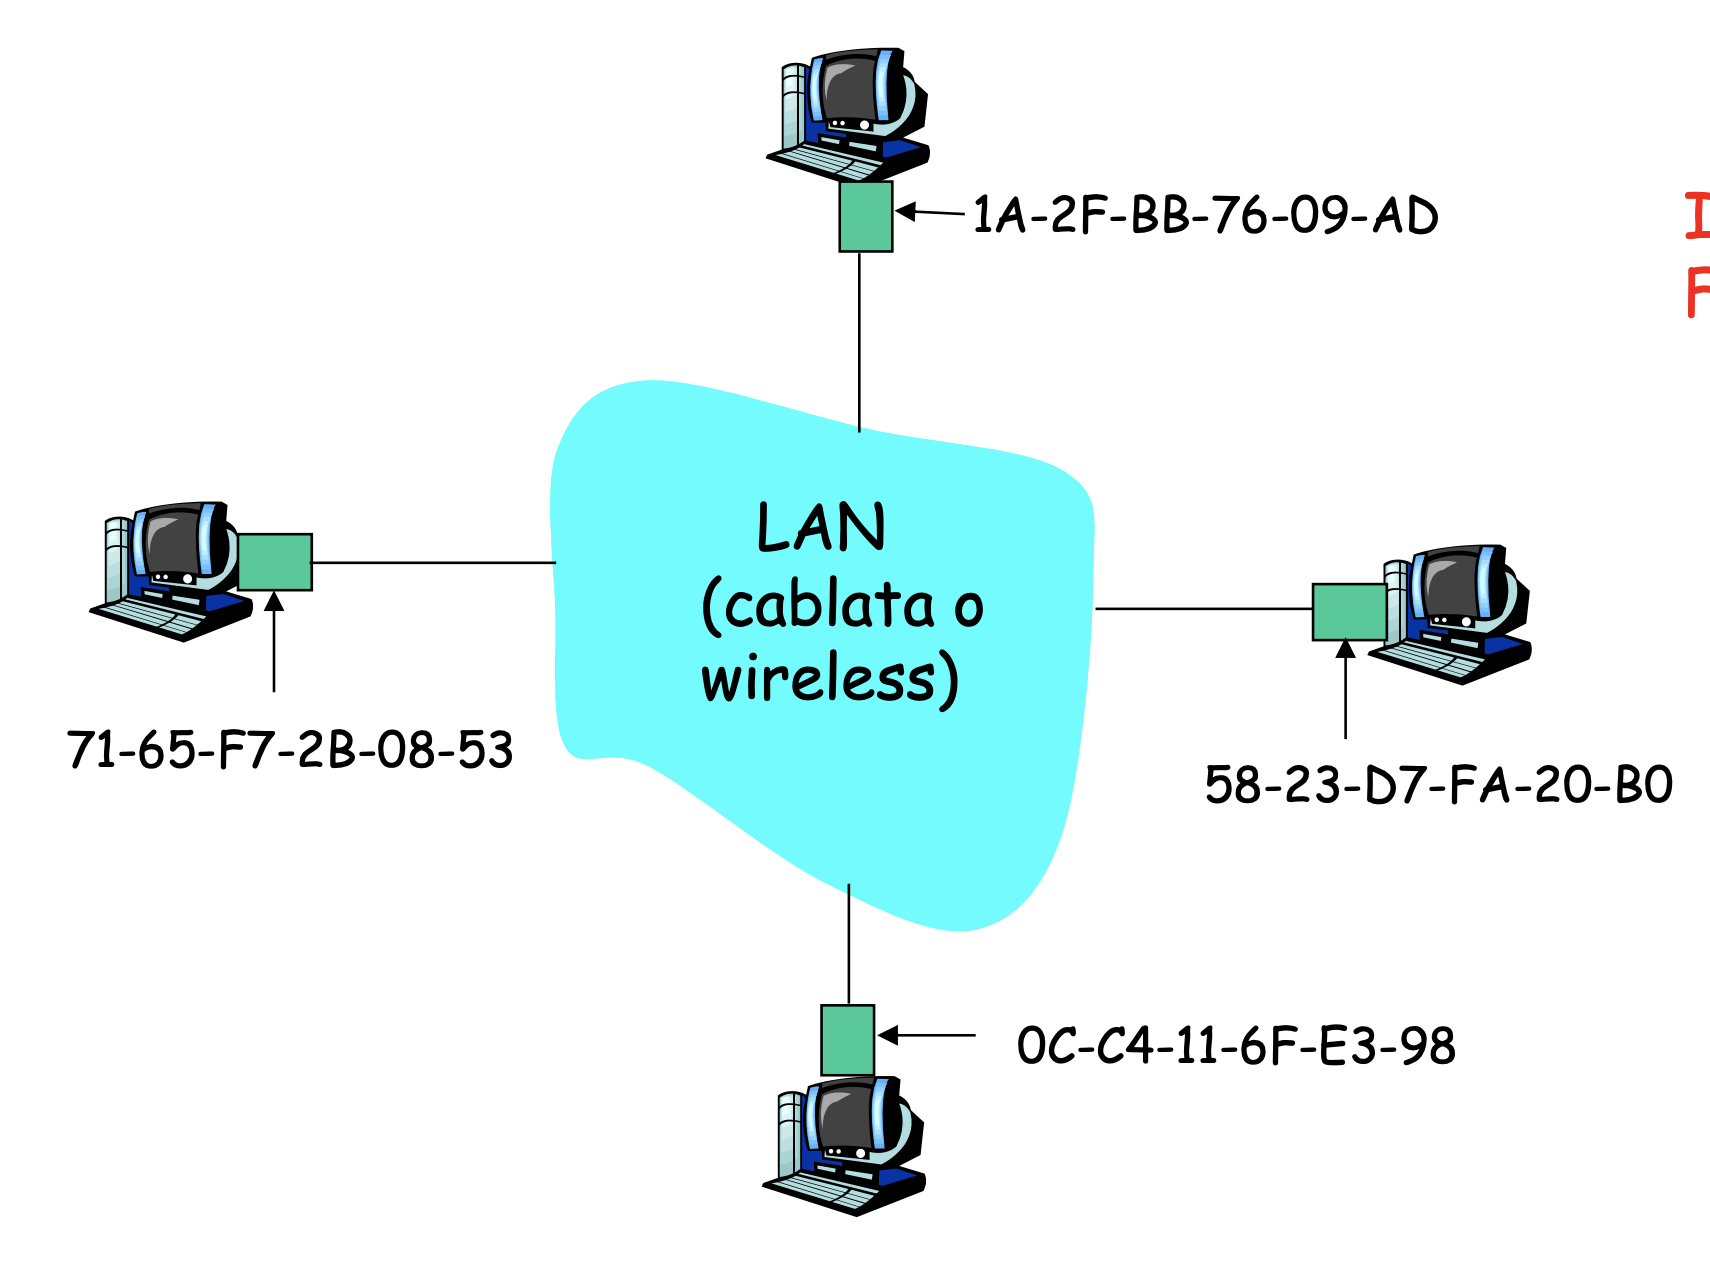
\includegraphics[width=0.7\linewidth]{arp}
	\end{center}

Sono gestiti dalla \textbf{IEEE} che vende alle società costruttrici di
adattatori i blocchi di spazio di indirizzi. La società dovrà garantire
l'unicità degli indirizzi.

Il vantaggio dell'orizzontalità del MAC è la portabilità delle schede da
una rete all'altra (cambierà solo l'IP)

\hypertarget{header-n115}{%
\subsubsection{Protocollo per la risoluzione degli indirizzi
(ARP)}\label{header-n115}}

Ogni nodo IP nella LAN ha una tabella ARP, la quale contiene la
corrispondenza tra indirizzi IP e MAC.

\begin{verbatim}
<Indirizzo IP, Indirizzo MAC, TTL>
\end{verbatim}

Il TTL indica quando bisognerà eliminare una voce nella tabella
(tipicamente 20 minuti).

\hypertarget{header-n119}{%
\paragraph{ARP nella stessa sottorete}\label{header-n119}}

ARP è plug-and-play: la tabella si costruisce automaticamente, non è
necessario l'intervento dell'amministratore di rete. Un nodo trasmette
in broadcast il messaggio di richiesta ARP, richiedendo l'indirizzo di
un secondo nodo. Quando quest'ultimo riceve il pacchetto ARP risponderà
comunicando il proprio indirizzo MAC.

\hypertarget{header-n121}{%
\paragraph{Invio verso un nodo esterno alla
sottorete}\label{header-n121}}

Se si vuole inviare un pacchetto da A a B attraverso un router R, il
router stesso avrà due tabelle ARP, una per ciascuna rete IP (LAN) a cui
è collegato.

\begin{enumerate}
\def\labelenumi{\arabic{enumi}.}
\item
  Il nodo A controlla qual'è la destinazione del suo datagram, se è
  nella sua stessa sottorete
\item
  A deve inoltrare il datagram al router R, deve quindi trovare il MAC
  dell'interfaccia del router utilizzando ARP
\item
  A quindi incapsulerà il datagram in un frame di livello 2 indirizzato
  a R, il quale toglierà l'header di livello 2, leggerà l'IP di
  destinazione e cercherà il percorso nella sua tabella di routing.
\item
  Il router R dovrà poi cercare l'indirizzo MAC del destinatario sulla
  seconda sottorete sempre con ARP
\item
  Infine il router R incapsulerà a sua volta il datagram in un frame di
  livello 2 inviandolo al destinatario.
\end{enumerate}

\begin{center}
		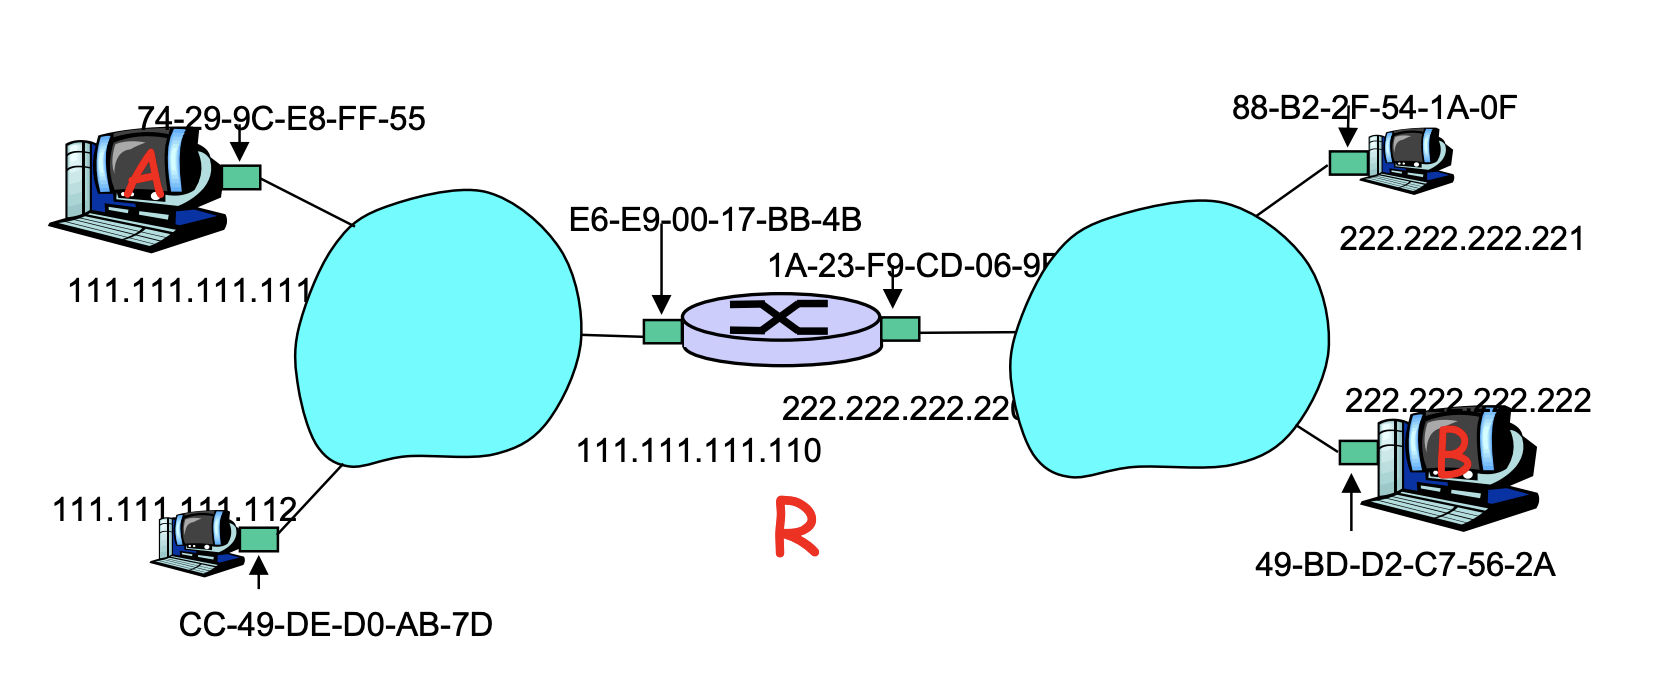
\includegraphics[width=0.7\linewidth]{arp2}
	\end{center}

\hypertarget{header-n135}{%
\section{Ethernet}\label{header-n135}}

Ethernet detiene una posizione dominante nel mercato delle LAN cablate:

\begin{itemize}
\item
  è stata la prima LAN ad alta velocità con vasta diffusione
\item
  Più semplice e meno costosa di token ring, FDDI e ATM
\item
  Al passo coi tempi con il tasso trasmissivo: da 10 Mbps finoa 10 Gbps
\end{itemize}

Il progetto originale di Ethernet fù ideato da Bob Metcalfe.

\hypertarget{header-n145}{%
\subsection{Topologia}\label{header-n145}}

La topologia originale era quella a Bus con cavo coassiale, diffusa fino
alla metà degli anni 90.

Le reti odierne seguono la topologia a stella, ogni nodo è collegato a
un hub o commutatore (\emph{switch}) permettendo di eseguire in ogni
nodo un protocollo Ethernet separato non entrando in collisione con
altri.

\begin{center}
		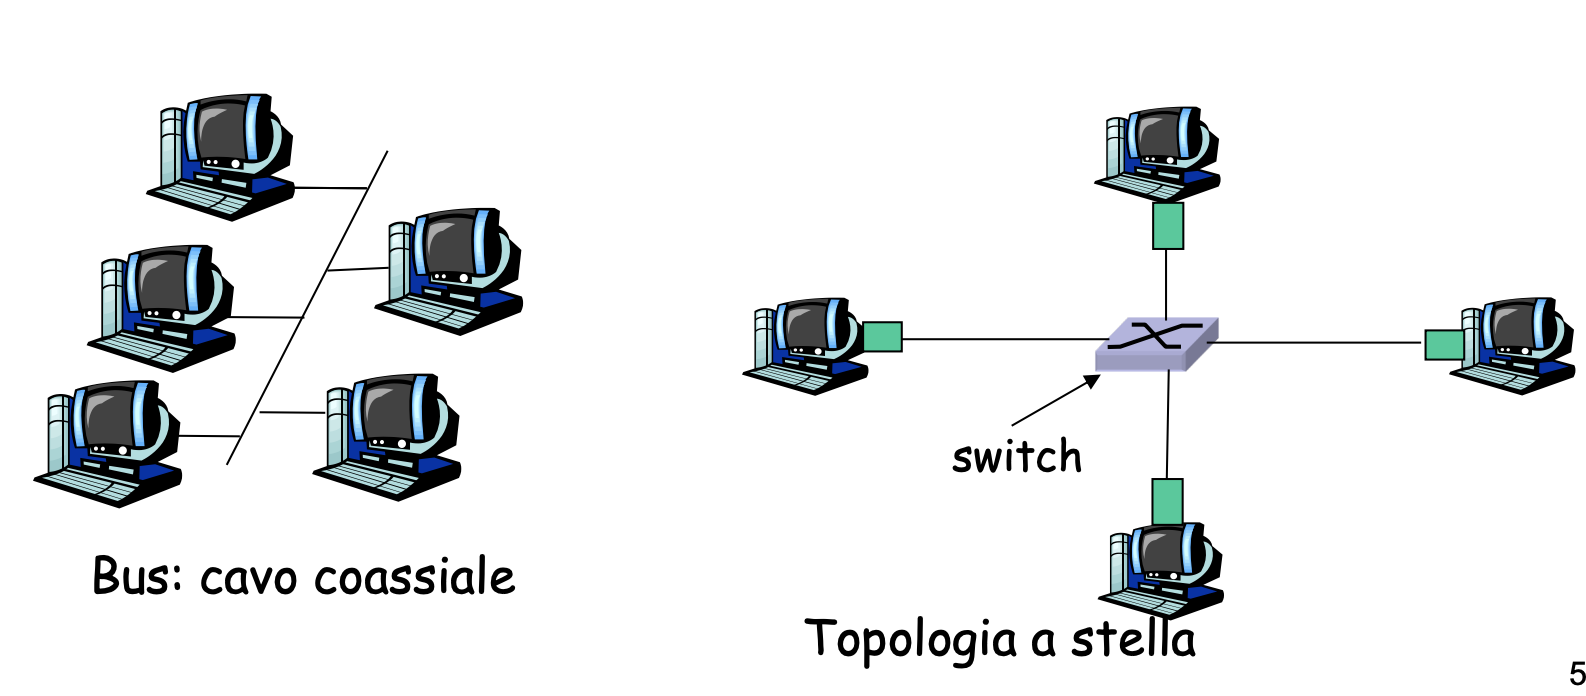
\includegraphics[width=0.7\linewidth]{topologie}
	\end{center}

\hypertarget{header-n149}{%
\subsection{Struttura dei pacchetti Ethernet}\label{header-n149}}

Preambolo, MAC di destinazione, MAC di origine, tipo, payload dati e CRC
(correzione degli errori).

\begin{itemize}
\item
  Il \textbf{preambolo} in specifico è costituito da 8 byte, i primi
  sette sono 10101010 e l'ultimo 10101011, e viene utilizzato per
  "attivare" il ricevitore quando viene inviato un pacchetto e per
  sincronizzare l'orologio con quello del trasmittente.
\item
  Gli \textbf{indirizzi} sono costituiti da 6 byte. Se è presente
  l'indirizzo di destinazione o il broadcast il payload viene trasferito
  direttamente al livello di rete altrimenti il pacchetto viene
  ignorato.
\item
  Il campo \textbf{tipo} consente a Ethernet di supportare i vari
  protocolli di rete (multiplexing).
\item
  Il controllo \textbf{CRC} consente all'adattatore ricevente di
  rilevare la presenza di un errore nei bit del pacchetto.
\end{itemize}

\begin{center}
		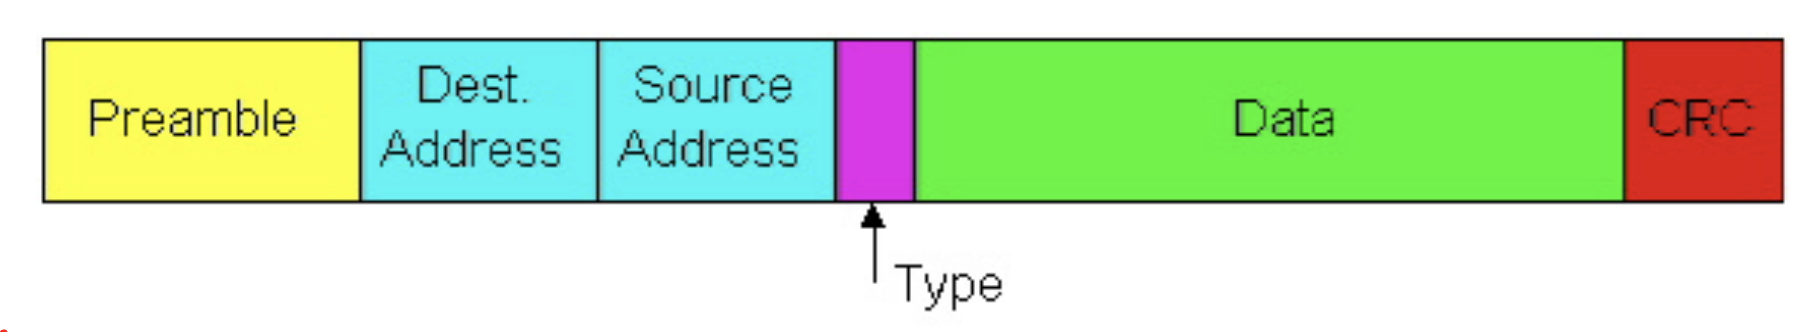
\includegraphics[width=0.7\linewidth]{ethernet}
	\end{center}

\hypertarget{header-n161}{%
\subsection{Servizio senza connessione non
affidabile}\label{header-n161}}

\begin{itemize}
\item
  \textbf{Senza connessione}: non è prevista nessuna forma di handshake
  preventiva prima di inviare un pacchetto.
\item
  \textbf{Non affidabile}: non esiste riscontro, il flusso dei datagram
  non è garantito poiché il compito viene delegato ai protocolli di
  livello superiore.
\end{itemize}

\hypertarget{header-n167}{%
\subsection{Fasi operative del protocollo CSMA/CD}\label{header-n167}}

\begin{enumerate}
\def\labelenumi{\arabic{enumi}.}
\item
  L'adattatore che riceve un datagram da livello 3 prepara il frame e
  ascolta il canale.
\item
  Se è inattivo inizia la trasmissione, altrimenti resta in attesa.
\item
  Durante la trasmissione, verifica se ci sono altri segnali provenienti
  da altri host.
\item
  Se rileva altri segnali interrompe la trasmissione e invia un segnale
  di disturbo (\emph{jam}) per avvisare della collisione.
\item
  L'adattatore si mette in attesa e viene definito uno slot di attesa
  pari a 512 bit; se viene messo in attesa successivamente l'intervallo
  raddoppia ogni volta. Dopo 10 volte raggiungerà il valore massimo,
  quando scade l'attesa se il canale è inattivo si potrà trasmettere
  nuovamente.
\end{enumerate}

Il segnale \emph{jam} viene trasmesso a un voltaggio più elevato ed è
lungo 48 bit. L'attesa è esponenziale con l'obiettivo di stimare quanti
sono i nodi in attesa coinvolti.

\hypertarget{header-n180}{%
\subsection{Efficienza di Ethernet}\label{header-n180}}

\begin{itemize}
\item
  Tempo di propagazione: tempo massimo che occorre al segnale per
  propagarsi tra due host
\item
  Tempo di trasmissione: tempo necessario per trasmettere un pacchetto
  della maggior dimensione possibile
\end{itemize}

\[efficienza = \frac{1}{1+5t_{prop}/t_{trasm}}\]

\begin{itemize}
\item
  Se il tempo di propagazione tende a 0, l'efficienza tenderà a 1
  (100\%, efficienza massima)
\item
  Per aumentare l'efficienza, in alternativa, si può aumentare il tempo
  di trasmissione.
\item
  Molto meglio di ALOHA: decentralizzato, semplice e poco costoso.
\end{itemize}

\hypertarget{header-n194}{%
\subsection{Ethernet 802.3}\label{header-n194}}

Sono presenti diversi standard Ethernet: il MAC e il frame sono
solitamente standard. Abbiamo però differenti velocità e differenti
mezzi trasmissivi (fibra o cavo).

\begin{center}
		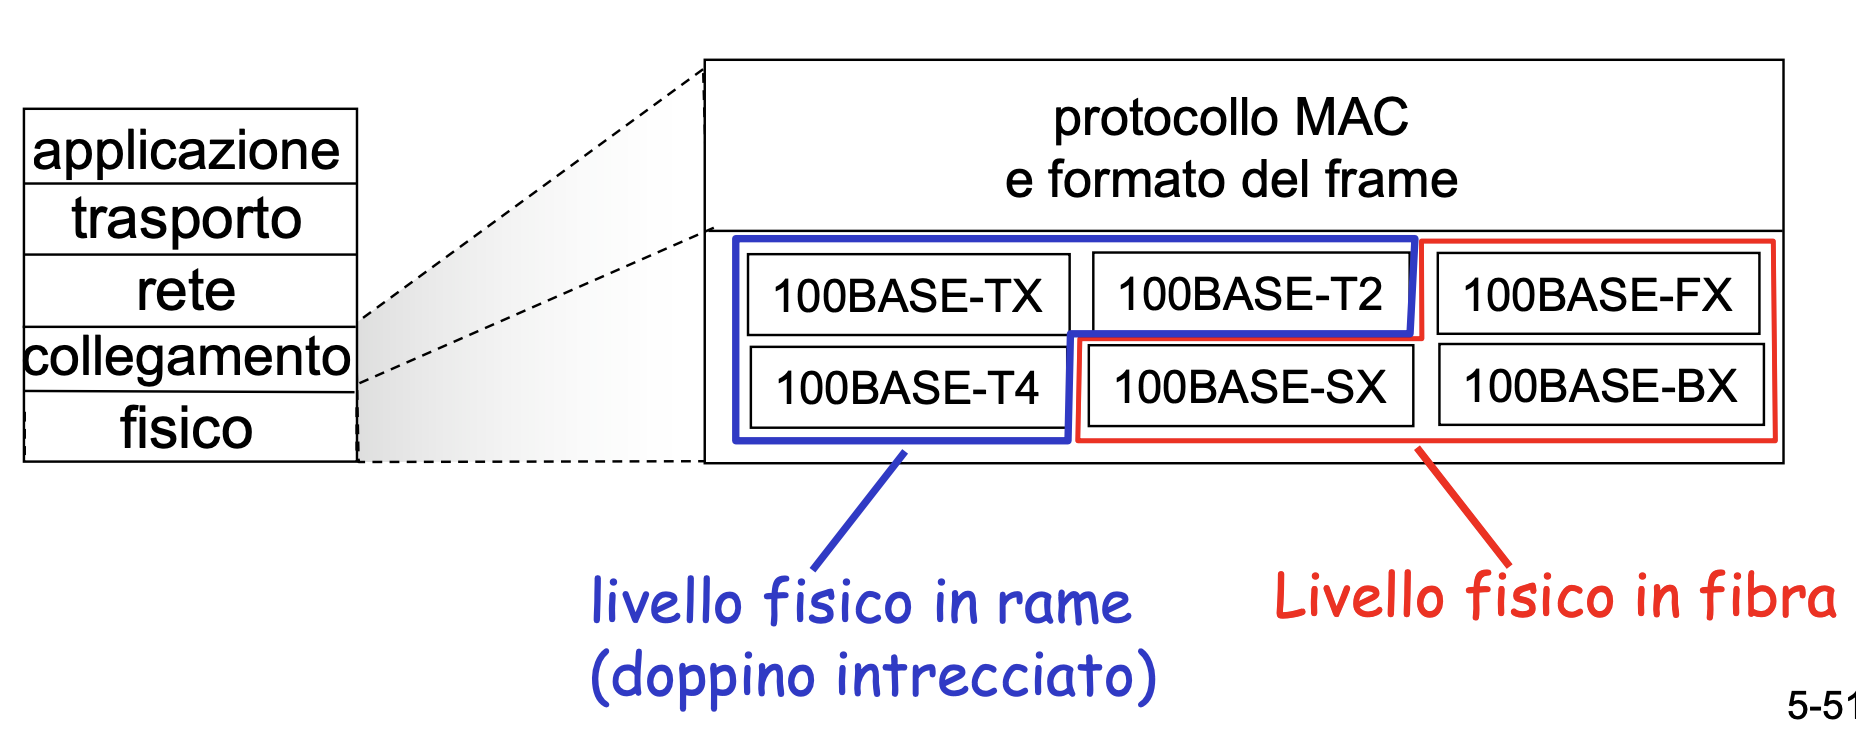
\includegraphics[width=0.7\linewidth]{fisico}
	\end{center}

\hypertarget{header-n197}{%
\subsection{Codifica Manchester}\label{header-n197}}

\begin{center}
		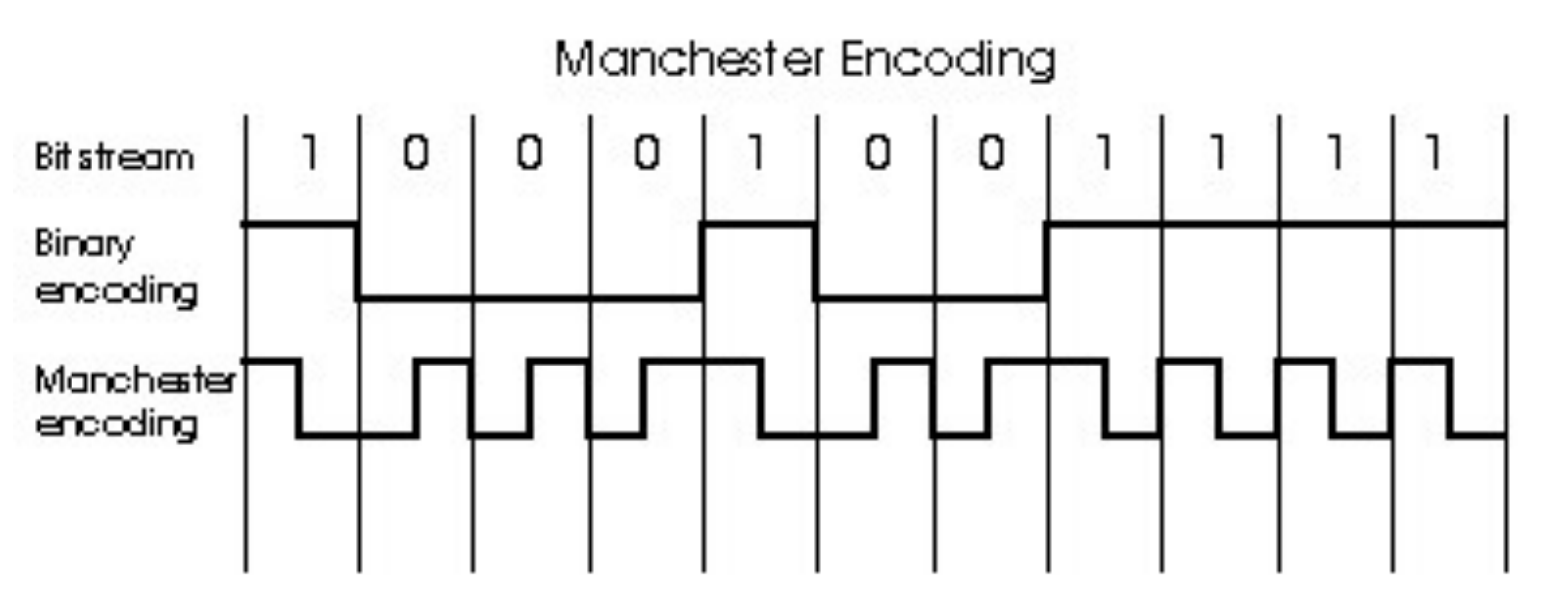
\includegraphics[width=0.7\linewidth]{manchester}
	\end{center}

La codifica Manchester veniva utilizzata in 10BaseT: durante la
ricezione di ciascun bit si verifica una transizione, permettendo di
sincronizzare gli orologi di trasmittenti e riceventi. L'operazione
veniva effettuata a livello fisico.

\hypertarget{header-n200}{%
\section{Switch a livello di collegamento}\label{header-n200}}

\hypertarget{header-n201}{%
\subsection{Hub}\label{header-n201}}

L'hub è un dispositivo "stupido" che opera sui singoli bit:

\begin{itemize}
\item
  riproduce un bit incrementandone l'energia trasmettendolo su tutte le
  interfacce, anche se su alcune c'è un segnale (avverrà una collisione)
\item
  non implementa rilevazione di portante né CSMA/CD
\end{itemize}

\hypertarget{header-n208}{%
\subsection{Switch}\label{header-n208}}

Lo switch è un dispositivo a livello di link, è più intelligente di un
hub e svolge un ruolo attivo:

\begin{itemize}
\item
  filtra e inoltra i pacchetti
\item
  ha una tabella e sa a quale porta inoltrare un pacchetto
\item
  è trasparente agli host
\item
  è un componente plug-and-play con autoapprendimento, non richiede
  l'intervento salvo configurazioni particolari
\end{itemize}

Lo switch consente più trasmissioni simultanee: i pacchetti vengono
infatti bufferizzati e il protocollo Ethernet viene implementato su
ciascun collegamento in entrata, evitando collisioni ma consentendo il
full-duplex. Grazie allo switching avvengono quindi più trasmissioni
simultaneamente.

\hypertarget{header-n220}{%
\subsubsection{Tabella di commutazione}\label{header-n220}}

Componente software utilizzato dallo switch per sapere dove inoltrare i
pacchetti ricevuti. Contiene il MAC del nodo di destinazione e
l'interfaccia associata, assomiglia alle tabelle di instradamento con la
differenza che può essere generata automaticamente dallo switch.

\hypertarget{header-n222}{%
\paragraph{Autoapprendimento}\label{header-n222}}

Quando riceve un pacchetto, lo switch impara l'indirizzo del mittente:
registrerà quindi nella tabella di switching la coppia indirizzo/porta.

\hypertarget{header-n224}{%
\subsubsection{Collegare gli switch}\label{header-n224}}

Gli switch possono essere interconnessi tra loro: gli host avranno la
sensazione di essere sulla stessa rete di livello 2 ma saranno su
differenti domini di collisione.

\hypertarget{header-n226}{%
\subsubsection{Esempio di rete di un'istituzione}\label{header-n226}}

\begin{center}
		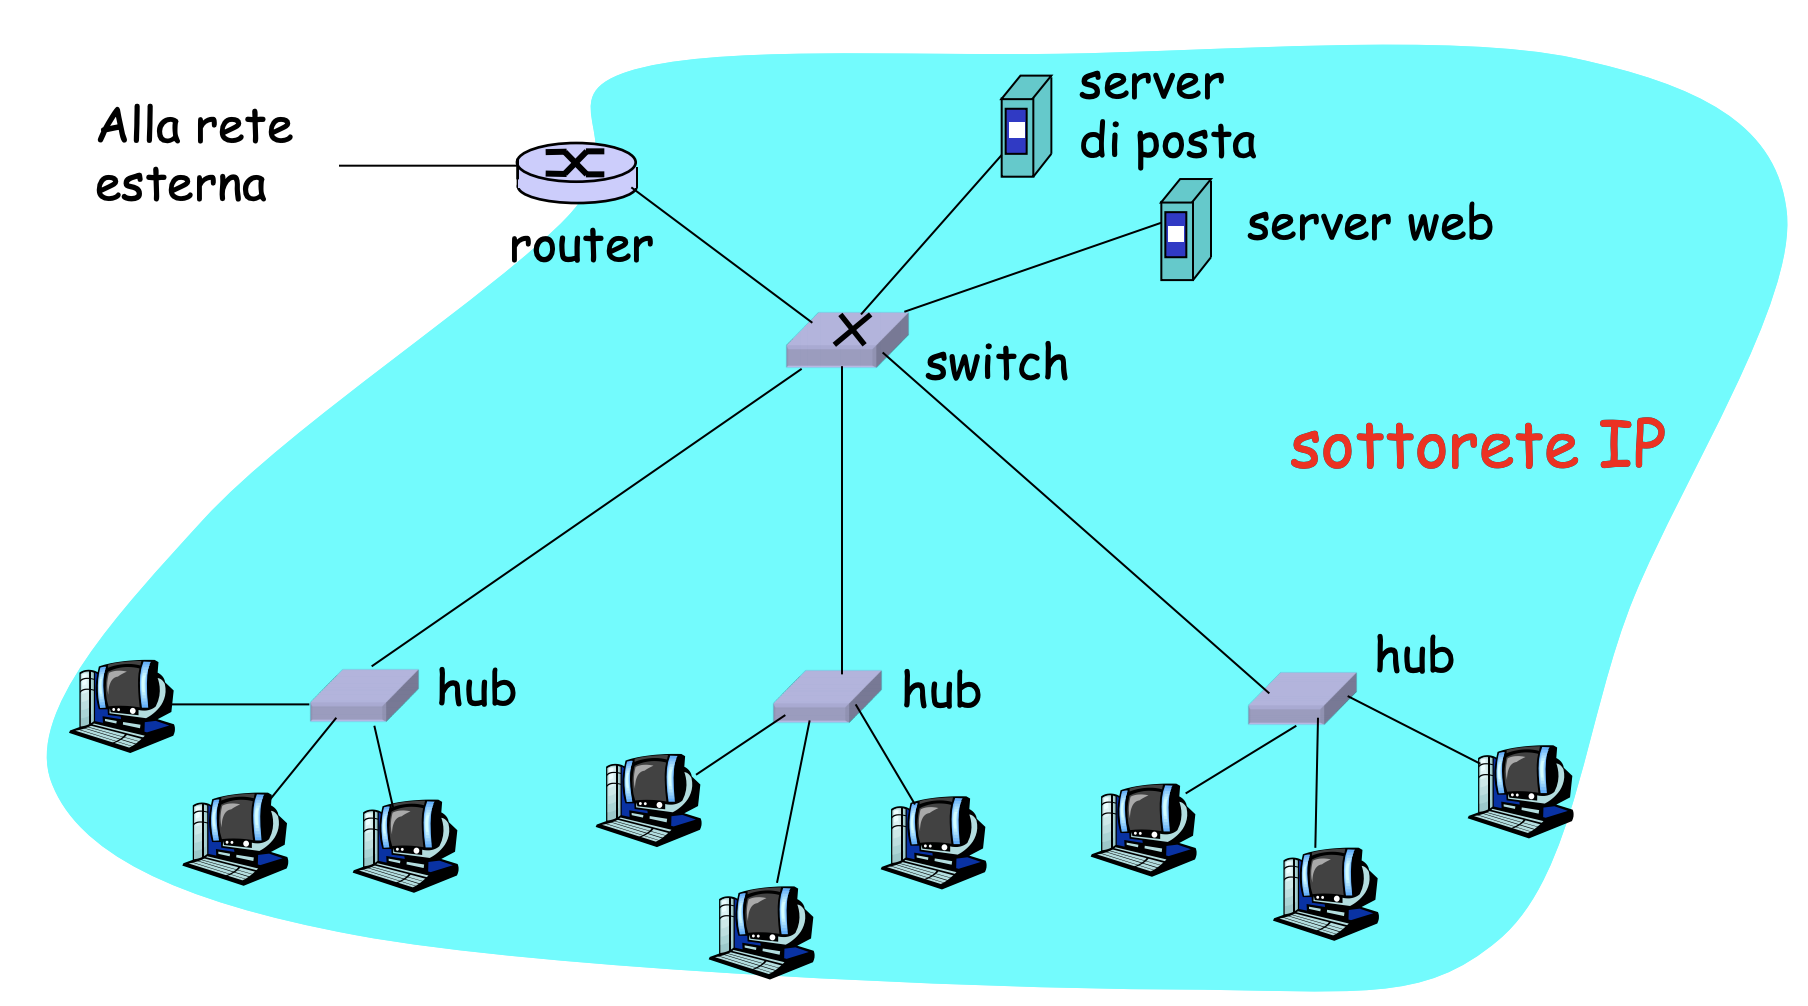
\includegraphics[width=0.7\linewidth]{istituzione}
	\end{center}

\hypertarget{header-n228}{%
\subsubsection{Switch e router a confronto}\label{header-n228}}

\begin{itemize}
\item
  Entrambi i dispositivi sono store-and-forward

  \begin{itemize}
  \item
    Il router lavora a livello di rete (dominio di broadcast)
  \item
    Lo switch lavora a livello di collegamento (dominio di collisione)
  \end{itemize}
\item
  I router mantengono tabelle d'inoltro e implementano algoritmi
  d'instradamento
\item
  Gli switch mantengono tabelle di commutazione e implementano il
  filtraggio e algoritmi di autoapprendimento
\end{itemize}

\hypertarget{header-n241}{%
\section{PPP: protocollo punto-punto}\label{header-n241}}

Protocollo estremamente semplice, prevede un solo collegamento tra
mittente e destinatario. Non è necessario un protocollo di accesso al
mezzo, non occorre un indirizzo MAC esplicito, veniva usato soprattutto
nei collegamenti ISDN.

Sono presenti protocolli più complessi come \textbf{HDLC} (High-level
Data Link Control).

\hypertarget{header-n244}{%
\subsection{Requisiti di IETF (RFC 1547)}\label{header-n244}}

\begin{itemize}
\item
  \textbf{Framing dei pacchetti:} incapsulare il pacchetto di rete
  dentro una struttura riconoscibile a livello di link e a livello
  fisico
\item
  \textbf{Trasparenza: }non porre nessuna restrizione alla
  configurazione dei dati
\item
  \textbf{Rilevazione di errori}
\item
  \textbf{Disponibilità della connessione: }rilevare eventuali guasti
\item
  \textbf{Negoziazione degli indirizzi di rete: }necessario un
  protocollo per interagire con la rete per ottenere ad esempio un
  indirizzo IP
\end{itemize}

Le altre funzioni come correzione degli errori, controllo di flusso,
riordinamento dei pacchetti \textbf{sono delegati ai livelli superiori.}

\hypertarget{header-n257}{%
\subsection{Formato dei pacchetti dati PPP}\label{header-n257}}

\begin{itemize}
\item
  \textbf{Flag: }ogni pacchetto inizia e termina con un byte di valore
  \textbf{01111110}
\item
  \textbf{Indirizzo: }unico valore \textbf{11111111} broadcast (solo due
  entità che comunicano)
\item
  \textbf{Controllo: }unico valore, tutti i frame sono dello stesso tipo
\item
  \textbf{Protocollo: }qual è il protocollo di livello superiore cui
  appartengono i dati incapsulati
\end{itemize}

\begin{center}
		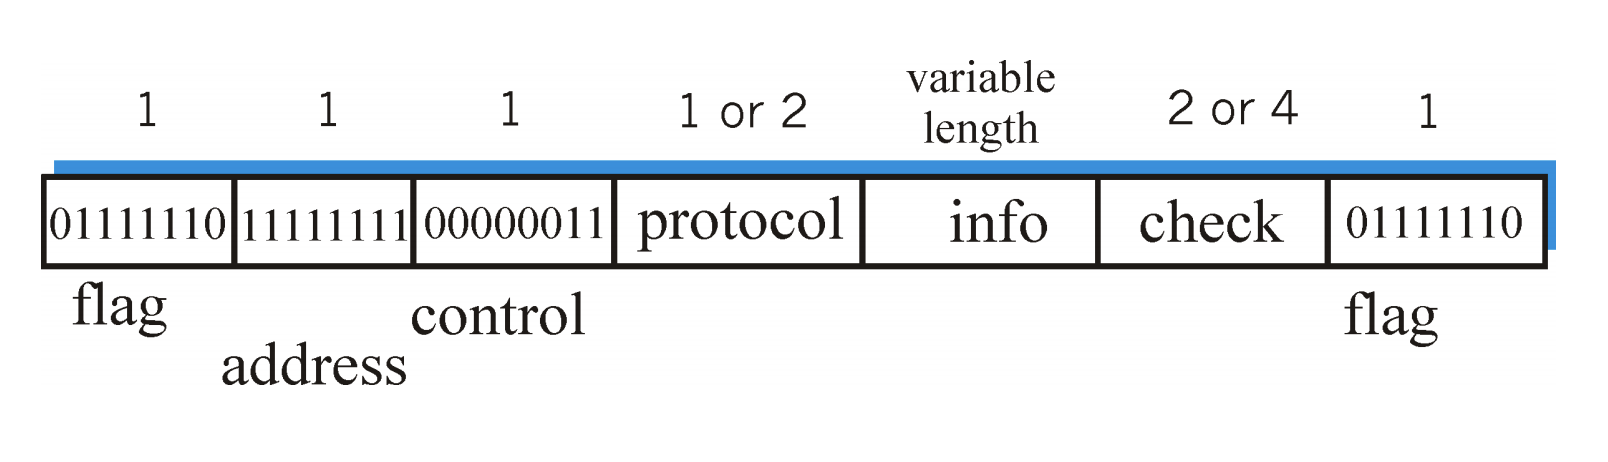
\includegraphics[width=0.7\linewidth]{ppp}
	\end{center}

\hypertarget{header-n268}{%
\subsubsection{Riempimento dei byte}\label{header-n268}}

Per il requisito di trasparenza non dev'essere possibile inserire nel
campo informazioni la stringa flag \textbf{01111110}, poiché non sarebbe
riconoscibile la fine del frame PPP.

Per ovviare a questo problema si ricorre alla tecnica del byte stuffing:
si aggiunge un byte di controllo pari al flag prima di ogni byte di
dati. In questo modo il destinatario riconoscerà la presenza di dati se
sono presenti due byte \textbf{01111110} consecutivi.

\begin{center}
		\includegraphics[width=0.7\linewidth]{byte-stuffing}
	\end{center}

\hypertarget{header-n272}{%
\section{Canali virtuali: una rete come un livello di
link}\label{header-n272}}

\hypertarget{header-n273}{%
\subsection{Il concetto di virtualizzazione}\label{header-n273}}

Per \textbf{virtualizzazione} si intende il processo di sostituzione di
una versione fisica con una rappresentazione software. Consente di
spezzare la dipendenza tra hardware e funzionalità software e una veloce
innovazione, è più facile testare e progettare i servizi senza il
bisogno dell'ambiente fisico. La virtualizzazione consente di isolare e
partizionare le risorse disponibili, oltre alla possibilità di maggior
controllo.

\hypertarget{header-n275}{%
\subsubsection{Tipi di virtualizzazione}\label{header-n275}}

\begin{itemize}
\item
  \textbf{Virtualizzazione hardware:} astrarre la funzionalità logica
  dall'infrastruttura fisica (ad esempio programmazione con compilatore)
\item
  \textbf{Virtualizzazione di rete: }reti virtuali basate su dispositivi
  virtuali, successivamente mappate su risorse fisiche
\item
  \textbf{Cloud: }gestire al meglio grosse quantità di CPU, storage e
  rete fornendo un pool di risorse aggregate, con lo scopo di fornire le
  risorse in maniera scalabile (illusione di risorse infinite)
\end{itemize}

\hypertarget{header-n283}{%
\subsubsection{Storia della virtualizzazione}\label{header-n283}}

La virtualizzazione inizia nell'era nei mainframe negli anni '60 dove le
risorse di computazione venivano condivise tra molti utenti.
Successivamente la virtualizzazione venne utilizzata nei datacenter,
consentendo la suddivisione delle risorse disponibili, arrivando al
giorno d'oggi con la virtualizzazione delle reti.

\hypertarget{header-n285}{%
\subsection{Internet: virtualizzazione delle reti}\label{header-n285}}

Grazie all'indirizzamento IP e ai gateway divenne possibile collegare
tra loro reti diverse per configurazione tra loro che prima non potevano
comunicare. IP consente quindi di virtualizzare le reti.

\hypertarget{header-n287}{%
\subsubsection{Architettura di Cerf e Kahn}\label{header-n287}}

Propone un primo tipo di virtualizzazione, dove il livello 3 (IP) rende
tutto omogeneo, infatti il livello è necessariamente standard. La
virtualizzazione ha consentito di spezzare l'indirizzamento a livello
globale (livello 3) da quello locale (livello 2), virtualizzando le
tecnologie di livello 2 (cavo, satellite, 56K).

\hypertarget{header-n289}{%
\subsubsection{Ethernet e domini}\label{header-n289}}

\begin{itemize}
\item
  \textbf{Dominio di "collisione": }determinato dall'insieme degli host
  che possono risentire di una collisione generata da due postazione
  arbitraria
\item
  \textbf{Dominio di "broadcast": }insieme degli host che ricevono i
  pacchetti in broadcast
\end{itemize}

\begin{center}
		\includegraphics[width=0.7\linewidth]{domini}
	\end{center}

\hypertarget{header-n296}{%
\subsection{LAN virtuali}\label{header-n296}}

Consente di definire più reti locali virtuali distinte utilizzando una
stessa infrastruttura fisica. Ogni VLAN si comporta come una rete locale
separata dalle altre:

\begin{itemize}
\item
  i pacchetti di broadcast sono confinati all'interno della VLAN
\item
  la comunicazione a livello 2 è confinata all'interno della VLAN
\item
  l'interconnessione tra più VLAN viene effettuata a livello 3 (è
  necessario un router)
\end{itemize}

Le VLAN sono definite nello standard 802.1q e nel 802.1d che riguarda la
comunicazione tra diversi standard 802 attraverso bridge.

\hypertarget{header-n306}{%
\subsubsection{Scopo delle VLAN}\label{header-n306}}

L'utilizzo delle VLAN consente:

\begin{itemize}
\item
  \textbf{risparmio: }definire più topologie virtuali utilizzando la
  stessa infrastruttura fisica. Non sono necessarie modifiche
  all'hardware
\item
  \textbf{aumento di prestazioni: }costruire la rete in base alle
  esigenze del momento, limitando il traffico broadcast
\item
  \textbf{aumento della sicurezza: }suddividere il traffico e isolarlo
  nelle varie VLAN
\item
  \textbf{flessibilità: }più facile spostare un utente dal punto di
  vista logico da una VLAN a un'altra
\end{itemize}

\hypertarget{header-n317}{%
\subsubsection{Requisiti sui bridge}\label{header-n317}}

Per implementare le VLAN è necessario che gli apparati supportino lo
standard 802.1q, con il quale è possibile definire due tipologie di
VLAN: la port based (privata) e quella tagged (802.1q).

Bisogna anche istruire bridge e switch perché riconoscano le VLAN, non è
possibile farlo in autoapprendimento ma vanno preprogrammati.

\hypertarget{header-n320}{%
\subsubsection{Funzioni del bridge in 802.1q}\label{header-n320}}

Per supportare le VLAN è necessario che i bridge svolgano le seguenti
tre funzioni:

\begin{itemize}
\item
  \textbf{ingress: }l'apparato deve capire a quale VLAN appartiene il
  frame in ingresso
\item
  \textbf{forwarding: }effettuare l'inoltro in base alla VLAN di
  appartenenza
\item
  \textbf{egress: }deve poter trasmettere il frame in uscita in modo che
  la VLAN sia interpretabile dagli altri bridge
\end{itemize}

\hypertarget{header-n329}{%
\subsubsection{Port based VLAN (untagged)}\label{header-n329}}

Tecnica abbastanza semplice, assegna in maniera statica ciascuna porta
del bridge a una VLAN definita con la configurazione del bridge.
Permette di costruire su un singolo apparato 2 o più bridge logici.

Le funzioni del bridge sono semplici:

\begin{itemize}
\item
  ingress: un frame in ingresso appartiene alla VLAN a cui è assegnata
  la porta
\item
  forwarding: frame inoltrato solamente verso le porte appartenenti alla
  stessa VLAN (forwarding database distinto per ogni VLAN)
\item
  egress: determinata la porta il frame viene trasmesso così com'è
\end{itemize}

Le VLAN untagged non richiedono di modificare i pacchetti Ethernet
poiché viene definito tutto sul bridge (che dev'essere compatibile con
lo standard 802.1q).

\hypertarget{header-n340}{%
\subsubsection{VLAN 802.1q (tagged)}\label{header-n340}}

Con questo standard è possibile far condividere lo stesso link fisico da
tra VLAN differenti, stampando nel pacchetto di livello 2 la VLAN di
appartenenza, aggiungendo nel frame Ethernet 4 byte che trasportano le
informazioni sulla VLAN. Questo identificativo (VLAN tag) deve essere
uguale per tutti i bridge che saranno tutti programmati per riconoscere
tale VLAN.

\hypertarget{header-n342}{%
\paragraph{Frame Ethernet 802.1q}\label{header-n342}}

Vengono aggiunti 4 byte dopo gli indirizzi di sorgente e destinazione i
quali conterranno il \textbf{TPI} (Tag Protocol Identifier), che
specifica che il frame è aderente a 802.1q e il \textbf{TCI} (Tag
Control Information) che trasporta informazioni relative alla VLAN
(priorità, interconnessione e VLAN tag).

\begin{center}
		\includegraphics[width=0.7\linewidth]{frame-vlan}
	\end{center}

\hypertarget{header-n345}{%
\paragraph{Considerazioni sul frame}\label{header-n345}}

La modifica proposta da 802.1q richiede anche la modifica della
dimensione massima di 1518 bytes con l'aggiunta di due byte. Inoltre, il
campo TPI ha un valore non utilizzato come "protocol type" nei frame
Ethernet ordinari in modo che sia riconoscibile che il frame è di tipo
802.1q ma una scheda non compatibile non scarti il frame.

\hypertarget{header-n347}{%
\subsubsection{VLAN con switch/router}\label{header-n347}}

Molti produttori consentono di implementare all'interno degli switch
funzionalità di routing (livello 3), permettendo di interconnettere tra
loro diverse VLAN mantenendo la separazione dei domini di broadcast.

Utilizzando porte configurate in modalità TRUNK è possibile trasportare
su un unico cavo i dati di più VLAN, lasciando agli switch il compito di
inoltrare i pacchetti correttamente.

\hypertarget{header-n350}{%
\subsubsection{Porte tagged e untagged}\label{header-n350}}

Negli switch 802.1q tutte le porte devono essere associate a una o più
VLAN: se la porta è associata a una VLAN untagged i frame ricevuti non
trasporteranno tag ne lo trasporteranno i frame in uscita, il link su
tali porte si chiama \emph{access link}.

Se la porta è in modalità tagged, il link si chiamerà \emph{trunk link}
e la VLAN di appartenenza del frame sarà definita dal valore nel tag.

\hypertarget{header-n353}{%
\subsubsection{Protocol based VLAN}\label{header-n353}}

Esiste la possibilità di assegnare un frame a una VLAN in maniera
dinamica, sulla base di diversi parametri opportunamente configurati
negli apparati (richiesti particolarmente evoluti).

Viene effettuato il packet filtering in base a delle regole come IP del
mittente, protocol type, indirizzo Ethernet. Può essere definita una
associazione statica, che avrà precedenza sulle altre regole.

Alcuni protocolli proprietari consentono di configurare le regole
dinamiche in maniera centrale, importando le configurazioni tramite la
rete, ad esempio non consentire l'accesso alle VLAN se il MAC address
dell'host non è stato registrato dall'amministratore di rete.

\hypertarget{header-n357}{%
\subsubsection{Default VLAN}\label{header-n357}}

Gli switch 802.1q sono preconfigurati con una default VLAN assegnata col
tag 1 e tutte le porte assegnate ad essa in modalità untagged,
permettendo al primo accesso di tale switch un funzionamento
tradizionale. Per poter modificare il VLAN ID associato a ciascuna porta
bisognerà eliminare tale porta dalla VLAN per poi poterla riconfigurare.

\hypertarget{header-n359}{%
\subsubsection{VLAN di management}\label{header-n359}}

In ogni rete IP sono presenti due piani di funzionalità: un piano dati
(o data plane) dove circola il traffico degli utenti e un piano di
controllo (control plane) relativo al traffico di controllo della rete
(BGP).

Usando le VLAN è interessante poter creare una VLAN relativa alla
gestione della rete, utilizzando la stessa infrastruttura.

\hypertarget{header-n362}{%
\subsection{ATM e MPLS}\label{header-n362}}

ATM e MPLS sono delle soluzioni che consentono di generare circuiti
virtuali utilizzando l'approccio a commutazione di pacchetto, consentono
l'allocazione delle risorse per i flussi e la gestione della qualità del
servizio. Queste tecnologie possono essere integrate nelle reti IP,
attualmente sono utilizzate per interconnettere alcune zone della rete e
non sono visibili all'utente.

\hypertarget{header-n364}{%
\subsubsection{Trasferimento asincrono (ATM)}\label{header-n364}}

ATM è nato verso metà anni 80 con l'obbiettivo di estendere la
tecnologia delle reti telefoniche in modo tale da essere utilizzata per
reti dati, progettando reti in grado di trasportare file audio e video
in tempo reale e supportare file di testo e immagini. Può essere
considerata la tecnologia telefonica di ultima generazione e viene
tutt'ora usata nelle reti ADSL, consente la realizzazione di circuiti
virtuali e l'implementazione del QoS.

\hypertarget{header-n366}{%
\paragraph{Architettura ATM}\label{header-n366}}

\begin{center}
		\includegraphics[width=0.7\linewidth]{atm}
	\end{center}

Segue la struttura TCP/IP, i terminali hanno 3 livelli mentre gli switch
2. I 3 livelli sono:

\begin{itemize}
\item
  \textbf{AAL (ATM adaptation layer): }presente nei dispositivi alla
  periferia della rete, svolge una funzione analoga al livello di
  Trasporto quindi segmentazione e riassemblaggio dei pacchetti e
  mappatura dei flussi nelle tipologie di QoS
\item
  \textbf{ATM:} fulcro dell'architettura, considerato "livello di rete",
  definisce la struttura della cella ATM (pacchetto) e tutti i suoi
  campi
\item
  \textbf{Livello fisico}
\end{itemize}

La rete ATM inizialmente era concepita come una rete stand-alone, che
fosse in grado di trasportare dati "da una scrivania a un'altra",
venendo considerata una tecnologia di rete. Dopo l'affermazione dello
stack TCP/IP come standard di Internet, per far si che ATM si potesse
integrare nella reti IP venne messo al suo di sotto, diventando un
livello 2, o livello di link commutato (utilizzato solo in alcune reti
al di sotto di IP).

\begin{center}
		\includegraphics[width=0.7\linewidth]{atm-ip}
	\end{center}

\hypertarget{header-n378}{%
\subparagraph{AAL: ATM Adaptation Layer}\label{header-n378}}

Presente solo negli host terminali, adatta i livelli superiori al
livello ATM sottostante frammentandoli adeguatamente (come nella
segmentazione TCP in pacchetti IP).

Ci sono diverse tipologie (o profili) AAL che suggeriscono il QoS
richiesto:

\begin{itemize}
\item
  \textbf{AAL1:} servizio a tasso costante, CBR, come nei servizi
  tradizionali per il traffico telefonico
\item
  \textbf{AAL2:} servizio a tasso variabile, VBR, adeguato per la
  trasmissione di video MPEG
\item
  \textbf{AAL5:} servizio dati (datagram IP)
\end{itemize}

\hypertarget{header-n388}{%
\subparagraph{Livello ATM}\label{header-n388}}

Offre il servizio di trasporto di celle attraverso la rete ATM, analogo
al livello di rete IP con servizi però molto differenti.

\begin{center}
		\includegraphics[width=0.7\linewidth]{servizi-atm}
	\end{center}

Il livello ATM implementa una rete a pacchetto a circuiti virtuali,
chiamati \textbf{canali virtuali (VC)}, percorsi con un collegamento
diretto fra sorgente e destinazione. Ciascun pacchetto viene marchiato
con l'indicatore \textbf{VCI} cosicché ogni switch saprà come
interpretarlo. Al canale virtuale possono essere riservate
\textbf{risorse dedicate} come banda e buffer per garantire il QoS.

I canali virtuali possono essere \textbf{permanenti}, per connessioni di
lunga durata, utilizzati tra zone della rete lontane tra loro, oppure
\textbf{dinamici} (creati su richiesta).

L'utilizzo di canali virtuali ha il vantaggio di poter controllare
prestazioni e QoS, controllando la congestione della rete, ma ha gli
svantaggi che potrebbe non esserci un profilo per ogni tipologia di dato
da trasportare, e avendo un numero limitato di canali virtuali non è del
tutto scalabile. Nel caso di connessioni di breve durata la costruzione
del VC richiede tempo riducendo le prestazioni percepite.

La \textbf{cella ATM} è costituita da un'intestazione da 5 byte (VCI,
Payload Type, Priorità sulla perdita di cella, e byte di controllo
errore) e un carico utile da 48 byte, che consente una trasmissione più
efficace avendo dimensione fissa e un ritardo minore data la piccola
dimensione.

\hypertarget{header-n395}{%
\subparagraph{Livello fisico ATM}\label{header-n395}}

Suddiviso in due parti:

\begin{itemize}
\item
  \textbf{Transmission Convergence Sublayer (TCS):} adatta la cella
  creata da ATM al livello fisico sottostante creando il checksum,
  effettuando la delineazione della cella e consentendo la
  strutturazione del canale trasmettendo celle inattive se non ci sono
  dati da inviare (il canale fisico è come un nastro trasportatore di
  celle)
\item
  \textbf{Physical Medium Dependent:} dipende dal mezzo fisico
  utilizzato
\end{itemize}

Il livello fisico di ATM consente il funzionamento con diverse
tecnologie come SONET/SDH (reti ottiche sincrone), T1/T3 (fibra,
microonde e cavo) o mappare le celle ATM su canali non strutturati
(grazie alla delineazione di ATM).

\hypertarget{header-n403}{%
\paragraph{IP su ATM}\label{header-n403}}

\begin{center}
		\includegraphics[width=0.7\linewidth]{ip-su-atm}
	\end{center}

Quando si raggiunge un router di ingresso nella rete ATM, questo router
dovrà determinare come trasferire il datagramma attraverso la rete,
utilizzando l'indirizzo IP di destinazione per capire dove inoltrarlo e
utilizzando ARP per chiedere alla rete ATM di costruire il percorso
relativo.

Raggiunto il router di uscita verrà risalita la pila protocollare,
incontrando AAL5 che permetterà di ricostruire il datagramma IP e di
conseguenza la risalita del pacchetto IP e sua consegna.

Per il corretto funzionamento di IP su ATM sarà necessario quindi un
protocollo ARP dedicato ad ATM e dei router dotati di uno stack
protocollare e un'interfaccia di rete compatibili con lo standard.

\hypertarget{header-n408}{%
\subsubsection{Multiprotocol Label Switching (MPLS)}\label{header-n408}}

L'obiettivo iniziale del protocollo MPLS è quello di velocizzarre
l'inoltro IP usando un'etichetta di lunghezza stabilita (invece
dell'indirizzo di destinazione IP).

\begin{center}
		\includegraphics[width=0.7\linewidth]{mpls}
	\end{center}

I router a commutazione di etichetta (router MPLS) inviano i pacchetti
analizzando l'etichetta MPLS nella tabella d'instradamento, passando il
datagramma all'interfaccia corretta. Viene utilizzato un particolare
protocollo RSVP-TE (estensione di RSVP) per distribuire etichette tra
router, che consente l'invio di pacchetti lungo reti non utilizzabili
con IP standard. Questi router coesistono coi router "solo-IP".
	
	
\end{document}